\documentclass[12pt]{ociamthesis}  % default square logo 
% \documentclass[12pt,beltcrest]{ociamthesis} % use old belt crest logo
%\documentclass[12pt,shieldcrest]{ociamthesis} % use older shield crest logo

%load any additional packages

% ---- START OF CUSTOM CONFIGURATION ----

\usepackage{amssymb} % unknown
\usepackage{array} % unknown
\usepackage{courier} % give courier font to listings and also \texttt{}
\usepackage{xcolor} % add colors to text using \textcolor{red}{<text>}
\usepackage{amsmath} % unknown
\usepackage{ulem} % unknown
\usepackage{hyperref} % ability to add links using \href{<link>}{<label>}, also ability to make the contents page clickable. Also use \url{<link>}
\usepackage{xurl}
% Configure \url such that it will skip to the next line of the URL is too long
\usepackage{listings} % ability to print code using \begin{lstlisting}
\usepackage{graphicx} % ability to add image
\usepackage{tablefootnote} % ability to use table footnotes in table using command \tablefootnotes
\usepackage{multirow} % ability to merge rows using \mergerow
\usepackage{makecell} % ability to have line breaks inside tables
\usepackage{imakeidx} % add an index for the document
\usepackage{float} % to fix the position of tables, so that it won't go to another place
\usepackage{cleveref} % Create references to different chapters
\makeindex % add an index for the document
% configure hyperref, display the contents page as its usual black color
\hypersetup{ 
    colorlinks,
    citecolor=black,
    filecolor=black,
    linkcolor=black,
    urlcolor=black
}

% configure listings
\lstset{language=Python}
\lstset{basicstyle=\ttfamily,breaklines=true} %use courier as font, also make sure it skips to another line when the text is too long for one line

\setlength{\parindent}{0pt} % disable indent of first line of each paragraph
\graphicspath{ {./images/} } % configure graphicx

%  Configure cleveref
\crefformat{section}{\S#2#1#3} % see manual of cleveref, section 8.2.1
\crefformat{subsection}{\S#2#1#3}
\crefformat{subsubsection}{\S#2#1#3}

% Include javascript syntax highlighting
\definecolor{lightgray}{rgb}{.9,.9,.9}
\definecolor{darkgray}{rgb}{.4,.4,.4}
\definecolor{purple}{rgb}{0.65, 0.12, 0.82}

\lstdefinelanguage{JavaScript}{
  keywords={typeof, new, true, false, catch, function, return, null, catch, switch, var, if, in, while, do, else, case, break},
  keywordstyle=\bfseries,
  ndkeywords={class, export, boolean, throw, implements, import, this},
  ndkeywordstyle=\bfseries,
  identifierstyle=\color{black},
  sensitive=false,
  comment=[l]{//},
  morecomment=[s]{/*}{*/},
  commentstyle=\itshape,
%   stringstyle=\color{red}\ttfamily,
  morestring=[b]',
  morestring=[b]"
}

\lstdefinelanguage{pug}{
  keywords={typeof, true, false, catch, function, return, null, catch, switch, var, if, in, while, do, else, case, break, p, h1, h2, h3, h4, h5, h6, small, span, img, ul, ol, li, table, tr, td, br, extends, div, block},
  keywordstyle=\bfseries,
  ndkeywords={class, export, boolean, throw, implements, import, src, href, target, width, height},
  ndkeywordstyle=\bfseries,
  identifierstyle=\color{black},
  sensitive=false,
  comment=[l]{//-},
  morecomment=[s]{/*}{*/},
  commentstyle=\itshape,
%   stringstyle=\color{red}\ttfamily,
  morestring=[b]',
  morestring=[b]"
}

\lstdefinelanguage{bash}{
  keywords={npm, git, add, commit, push, clone, init, checkout, merge, cd, ls, rm, cp, mv, pwd, mkdir, touch},
  keywordstyle=\bfseries,
  ndkeywords={},
  ndkeywordstyle=\bfseries,
  identifierstyle=\color{black},
  sensitive=false,
  comment=[l]{//-},
  morecomment=[s]{/*}{*/},
  commentstyle=\itshape,
%   stringstyle=\color{red}\ttfamily,
  morestring=[b]',
  morestring=[b]"
}
% ---- END OF CUSTOM CONFIGURATION ----

%input macros (i.e. write your own macros file called mymacros.tex 
%and uncomment the next line)
%\include{mymacros}

\title{Web \& Git \\ (DRAFT)}   %note \\[1ex] is a line break in the title

\author{Oscar Mui }             %your name
\college{University College}  %your college

% \renewcommand{Notes for}{change the default text here if needed}
\degree{Learn to Code } %\\[1ex] (in Python)     %the degree
\degreedate{Hilary 2023}         %the degree date

%end the preamble and start the document
\begin{document}

%this baselineskip gives sufficient line spacing for an examiner to easily
%markup the thesis with comments
\baselineskip=18pt plus1pt

%set the number of sectioning levels that get number and appear in the contents
\setcounter{secnumdepth}{3}
\setcounter{tocdepth}{3}


\maketitle                  % create a title page from the preamble info

\begin{romanpages}          % start roman page numbering

\include{dedication}        % include a dedication.tex file
\include{acknowlegements}   % include an acknowledgements.tex file
\chapter*{Preface}

This piece of notes covers one way of building a \textbf{static} website. It facilitates my live teaching sessions or my Web \& Git YouTube series.
\vspace{6mm}

We use \textbf{Pug.js} (sometimes abbreviated to Pug in this piece of notes) instead of HTML, \textbf{less} instead of CSS. And used gulp to translate the files back to HTML and CSS. The generated HTML files can be directly opened by the browser. We also included \textbf{Bootstrap} to make our static website responsive.
\vspace{6mm}

At the same time, we will be learning how to use \textbf{Git} and \textbf{command line tools}.

\section{Prerequisites}

Basic coding experience (e.g. variables, loops) in any programming languages (e.g. C++, Python) is expected. Knowing basic HTML and CSS would be helpful, but not necessary. 
% I would contrast HTML with Pug.js and CSS with less throughout the notes, if you have not learned HTML and CSS you could skip those sessions.

\section{Way to read the notes}

This piece of notes aims to fill the gaps of the online resources, and also acts as the bridge between different components of the project. It will not include every detail that you need to know, but I would try to include different online resources (documentations and YouTube tutorials) required in the form of hyperlinks along the way.
\vspace{6mm}

Hands on practice is also super important in programming, instead of revising this piece of notes over and over again, you will probably learn more if you make more websites on your own. :)
\vspace{6mm}

We start with installing the tools you need for this project. It is probably a bit complicated for most of you, but I reassure you that it is worth the time. It also tells you some basic tips to use the project. In order for you to have hands on experience with coding as soon as possible, \cref{sec:pug1} introduces the Pug.js syntax allowing you to edit the content of the web page. Then we go back to some boring\footnote{I guess the command line interface is not colourful is what makes it boring?} details in chapters 3-6. Then we go back to talk about styling in chapters 7-8. Finally, we will learn how to use variables in Pug.js in \cref{sec:pug2}. And we conclude by miscellaneous bits in \cref{sec:misc}.
\vspace{6mm}

I marked the less essential sections with \textit{Advanced} or \textit{Of less importance}. The whole of \cref{sec:git2} and \cref{sec:pug2} are labelled with \textit{Advanced}, while the whole of \cref{sec:misc} is labelled with \textit{Of less importance}. You can read the sections without the markings first, then those with \textit{Advanced}, then those with \textit{Of less importance}.

\section{Why?}

Why are we learning how to make a website? Why this particular framework? Why are we learning Git and command line tools at the same time?

I decided to delay answering these questions until the last chapter \cref{sec:rationale}, as it is easier to explain after you have learnt all the knowledge. For now, you can just go ahead if you are motivated enough to do so. I wish you learn this also because you like it other than it being useful in some sense.
 
\section{A word of warning}

This is just a draft, aiming to include everything in the shortest amount of time possible, so explanations and examples may be inadequate. If there are any errors in the notes feel free to contact me by email oscar.mui@univ.ox.ac.uk

\section{Linktree}

Useful links related to the notes.
\vspace{6mm}

Video series I made: \textit{(I have to admit they are not of the best quality, and the series is not finished yet)}

\url{https://www.youtube.com/playlist?list=PLjGmdnqrOKuYXiu7lgG5HW71jPEUd1XCm}
\vspace{6mm}

Example website:

\url{https://numbersarefun.netlify.app/}
\vspace{6mm}

Template for you to start from scratch:

\url{https://github.com/KidProf/static-web-sandbox}
\vspace{6mm}

Source code of the finished website:

\url{https://github.com/KidProf/numbersarefun-sample-temp}
\vspace{6mm}

Pug.js: 

\url{https://pugjs.org/}
\vspace{6mm}

Less: 

\url{https://lesscss.org/}
\vspace{6mm}

Bootstrap: 

\url{https://getbootstrap.com/}
\vspace{6mm}

          % include the abstract


\tableofcontents            % generate and include a table of contents
% \listoffigures              % generate and include a list of figures
\end{romanpages}            % end roman page numbering

%now include the files of latex for each of the chapters etc
\chapter{Installation}

\textit{Covered in \href{https://www.youtube.com/watch?v=oIsH0V3fRt8&list=PLjGmdnqrOKuYXiu7lgG5HW71jPEUd1XCm&index=2}{video 1 of the series}}
\vspace{6mm}

Probably the most complicated installation procedure you have ever seen. However, it is only a one-time process. Those are essential tools for you to code more advanced stuff using JavaScript. It is also a good practice in using the command line interface.

\section*{For those of you not using Git}

You would still need to perform step \cref{sec:install1} if you are using a Windows machine.\footnote{Because the Windows CMD uses slightly different command keywords.}

You can download the code as a zip file \href{https://github.com/KidProf/static-web-sandbox}{here}.\footnote{Link: \url{https://github.com/KidProf/static-web-sandbox}}\textit{(see figure)} You do not need a GitHub account to do so. 

After that, proceed with step \cref{sec:install5}, and unzip your code inside the folder, then proceed with step \cref{sec:install7} and onwards.

\begin{figure}[h]
\centering
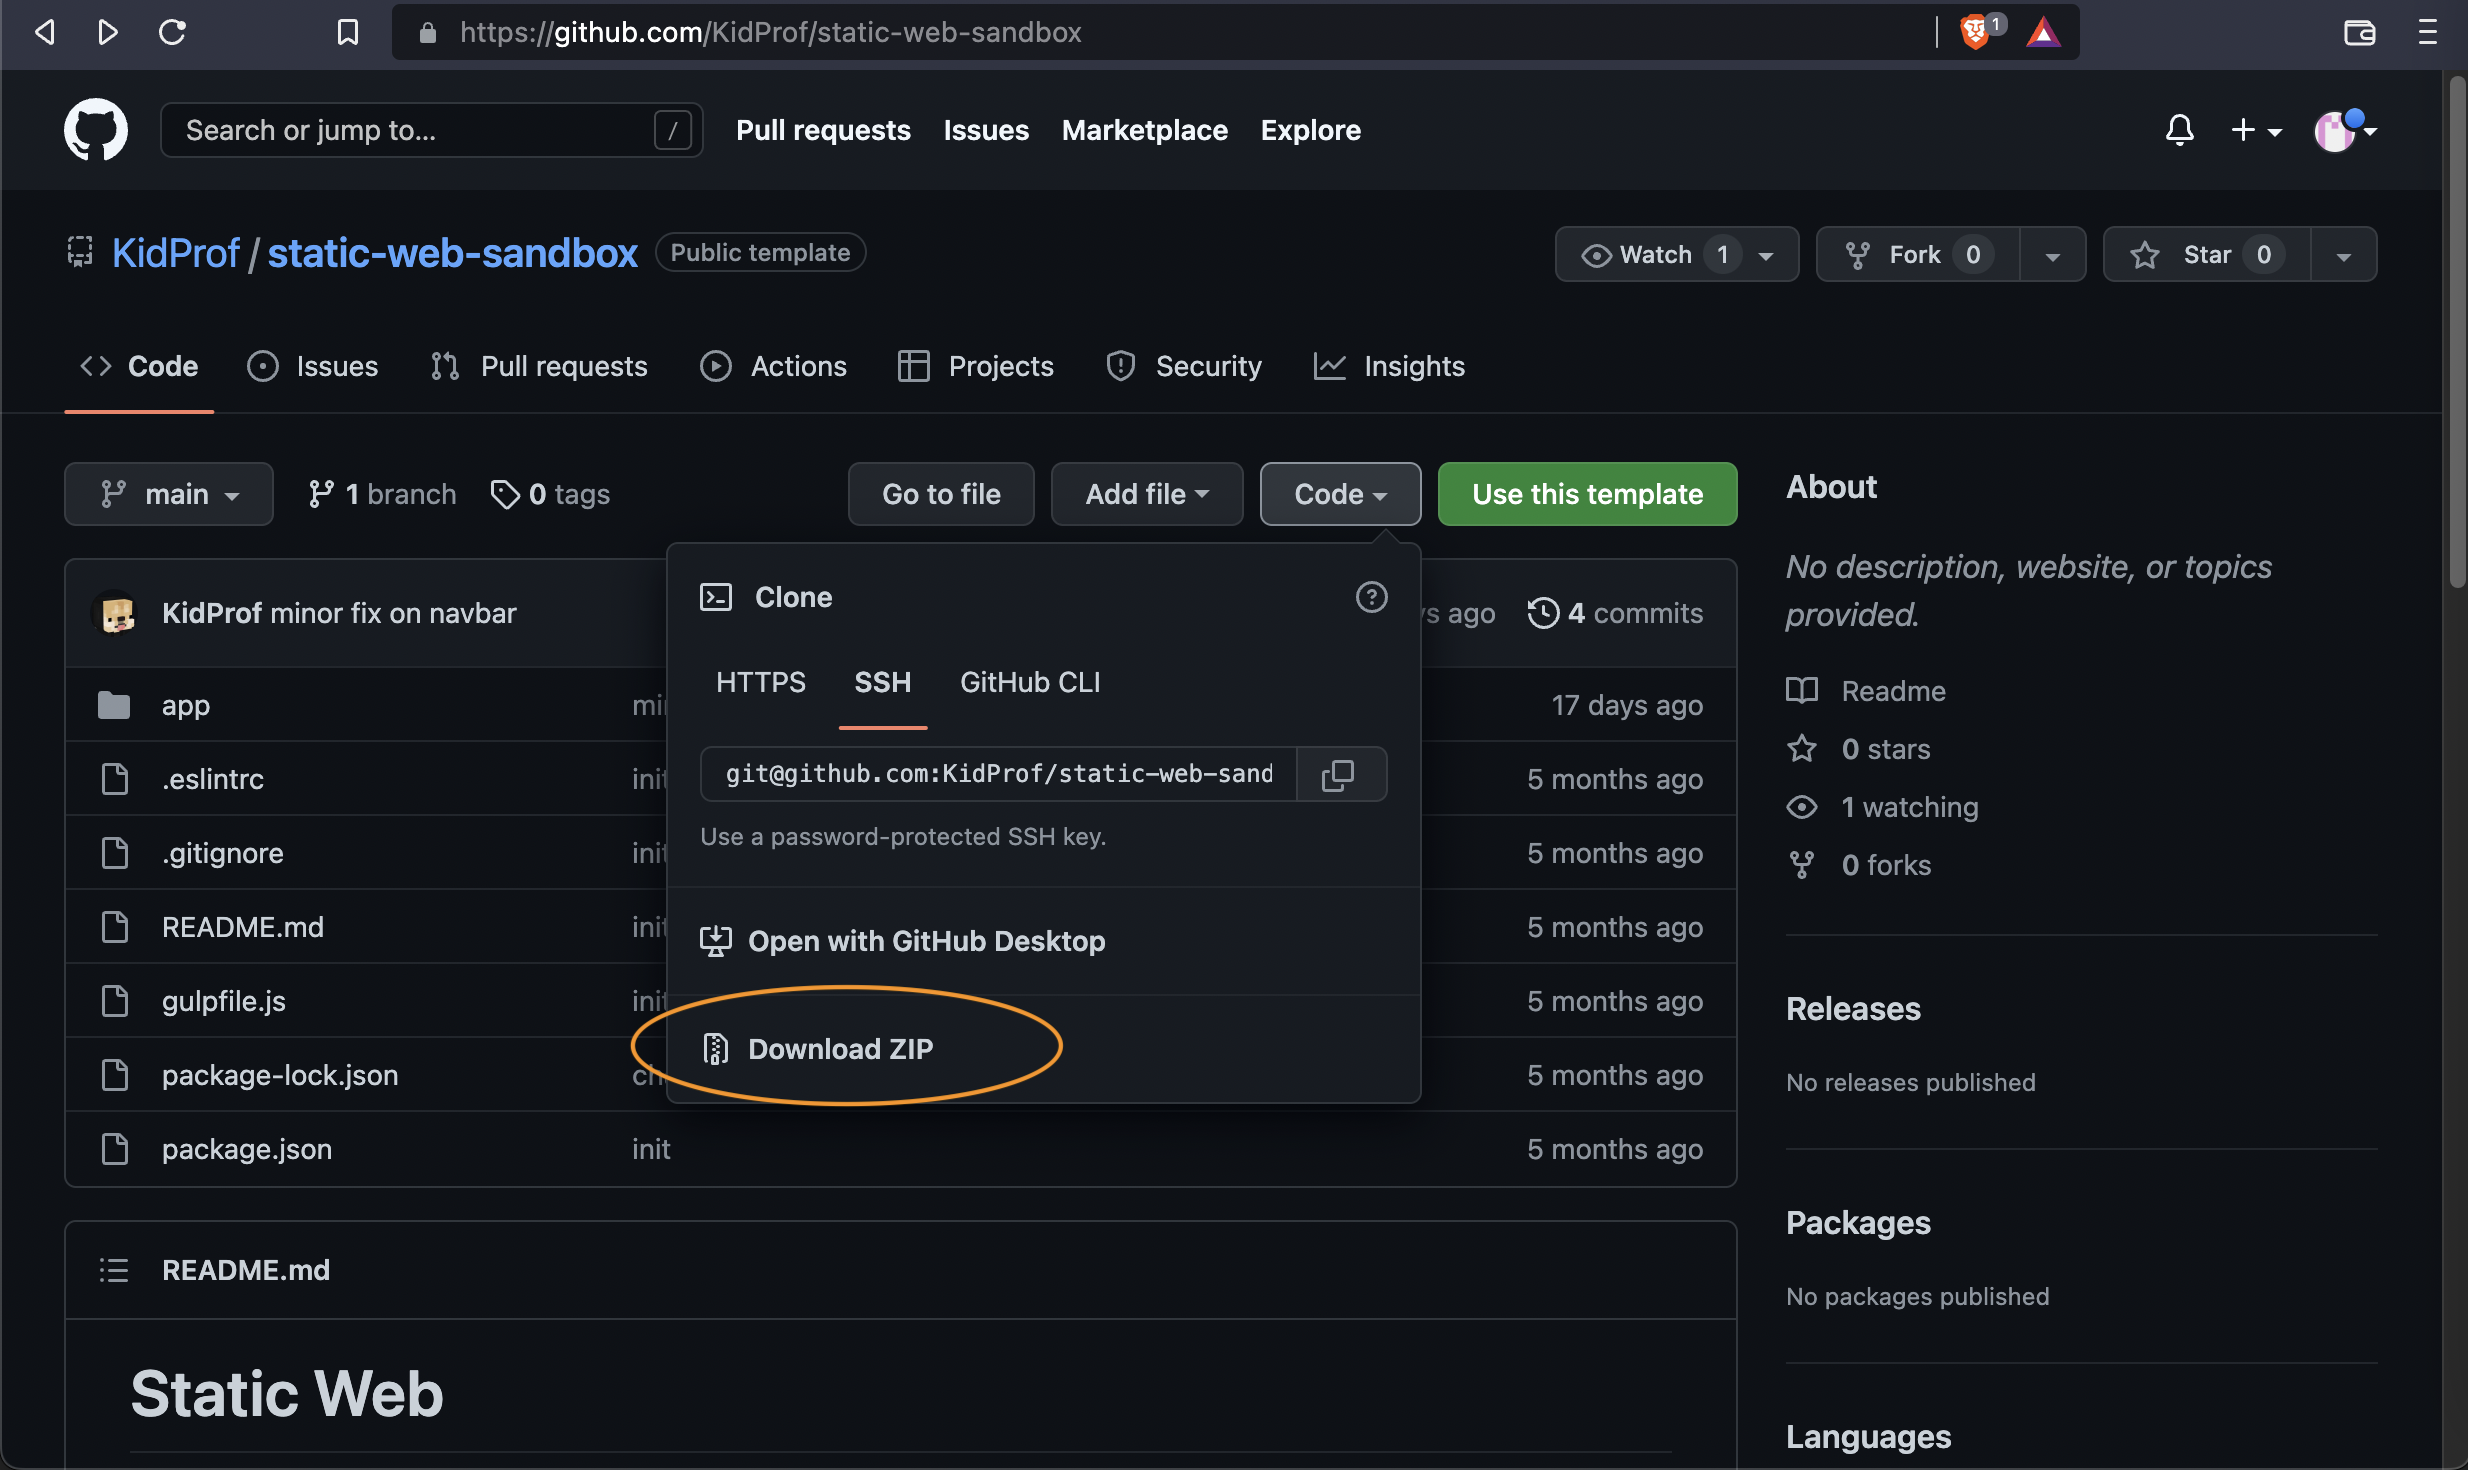
\includegraphics[width=15cm]{images/ch1-download-as-zip.png}
\caption{Screenshot from GitHub showing how to download the code by zip}
\end{figure}

\section{Git Bash (for Windows only)}
\label{sec:install1}

\textit{If you are using MacOS or Linux, skip to step 2: Creating a GitHub account}
\vspace{6mm}

Download Git Bash by following \href{https://git-scm.com/download/win}{this link}.\footnote{Link: \url{https://git-scm.com/download/win}} It should be straightforward.

\section{Creating a GitHub account}

Create your own GitHub account \href{https://github.com/}{here}.\footnote{Link: \url{https://github.com/}} It should be straightforward. Remember the email you used for registration.

\section{Creating a new repository using the template}

Open my template by following \href{https://github.com/KidProf/static-web-sandbox}{this link}.\footnote{Link: \url{https://github.com/KidProf/static-web-sandbox}} Then click the big green button \textit{Use this template}. You will be prompted to create a new repository. \textbf{Repository} is a fancier word for project, sometimes abbreviated to \textbf{repo}. Provide a repository name (a.k.a. project name) of your choice, preferably something meaningful; and you can set it either to public or private based on your own preference. You can change these two settings in the future. Do not change up any other settings in this page. \textit{(see figure)}

\begin{figure}[h]
\centering
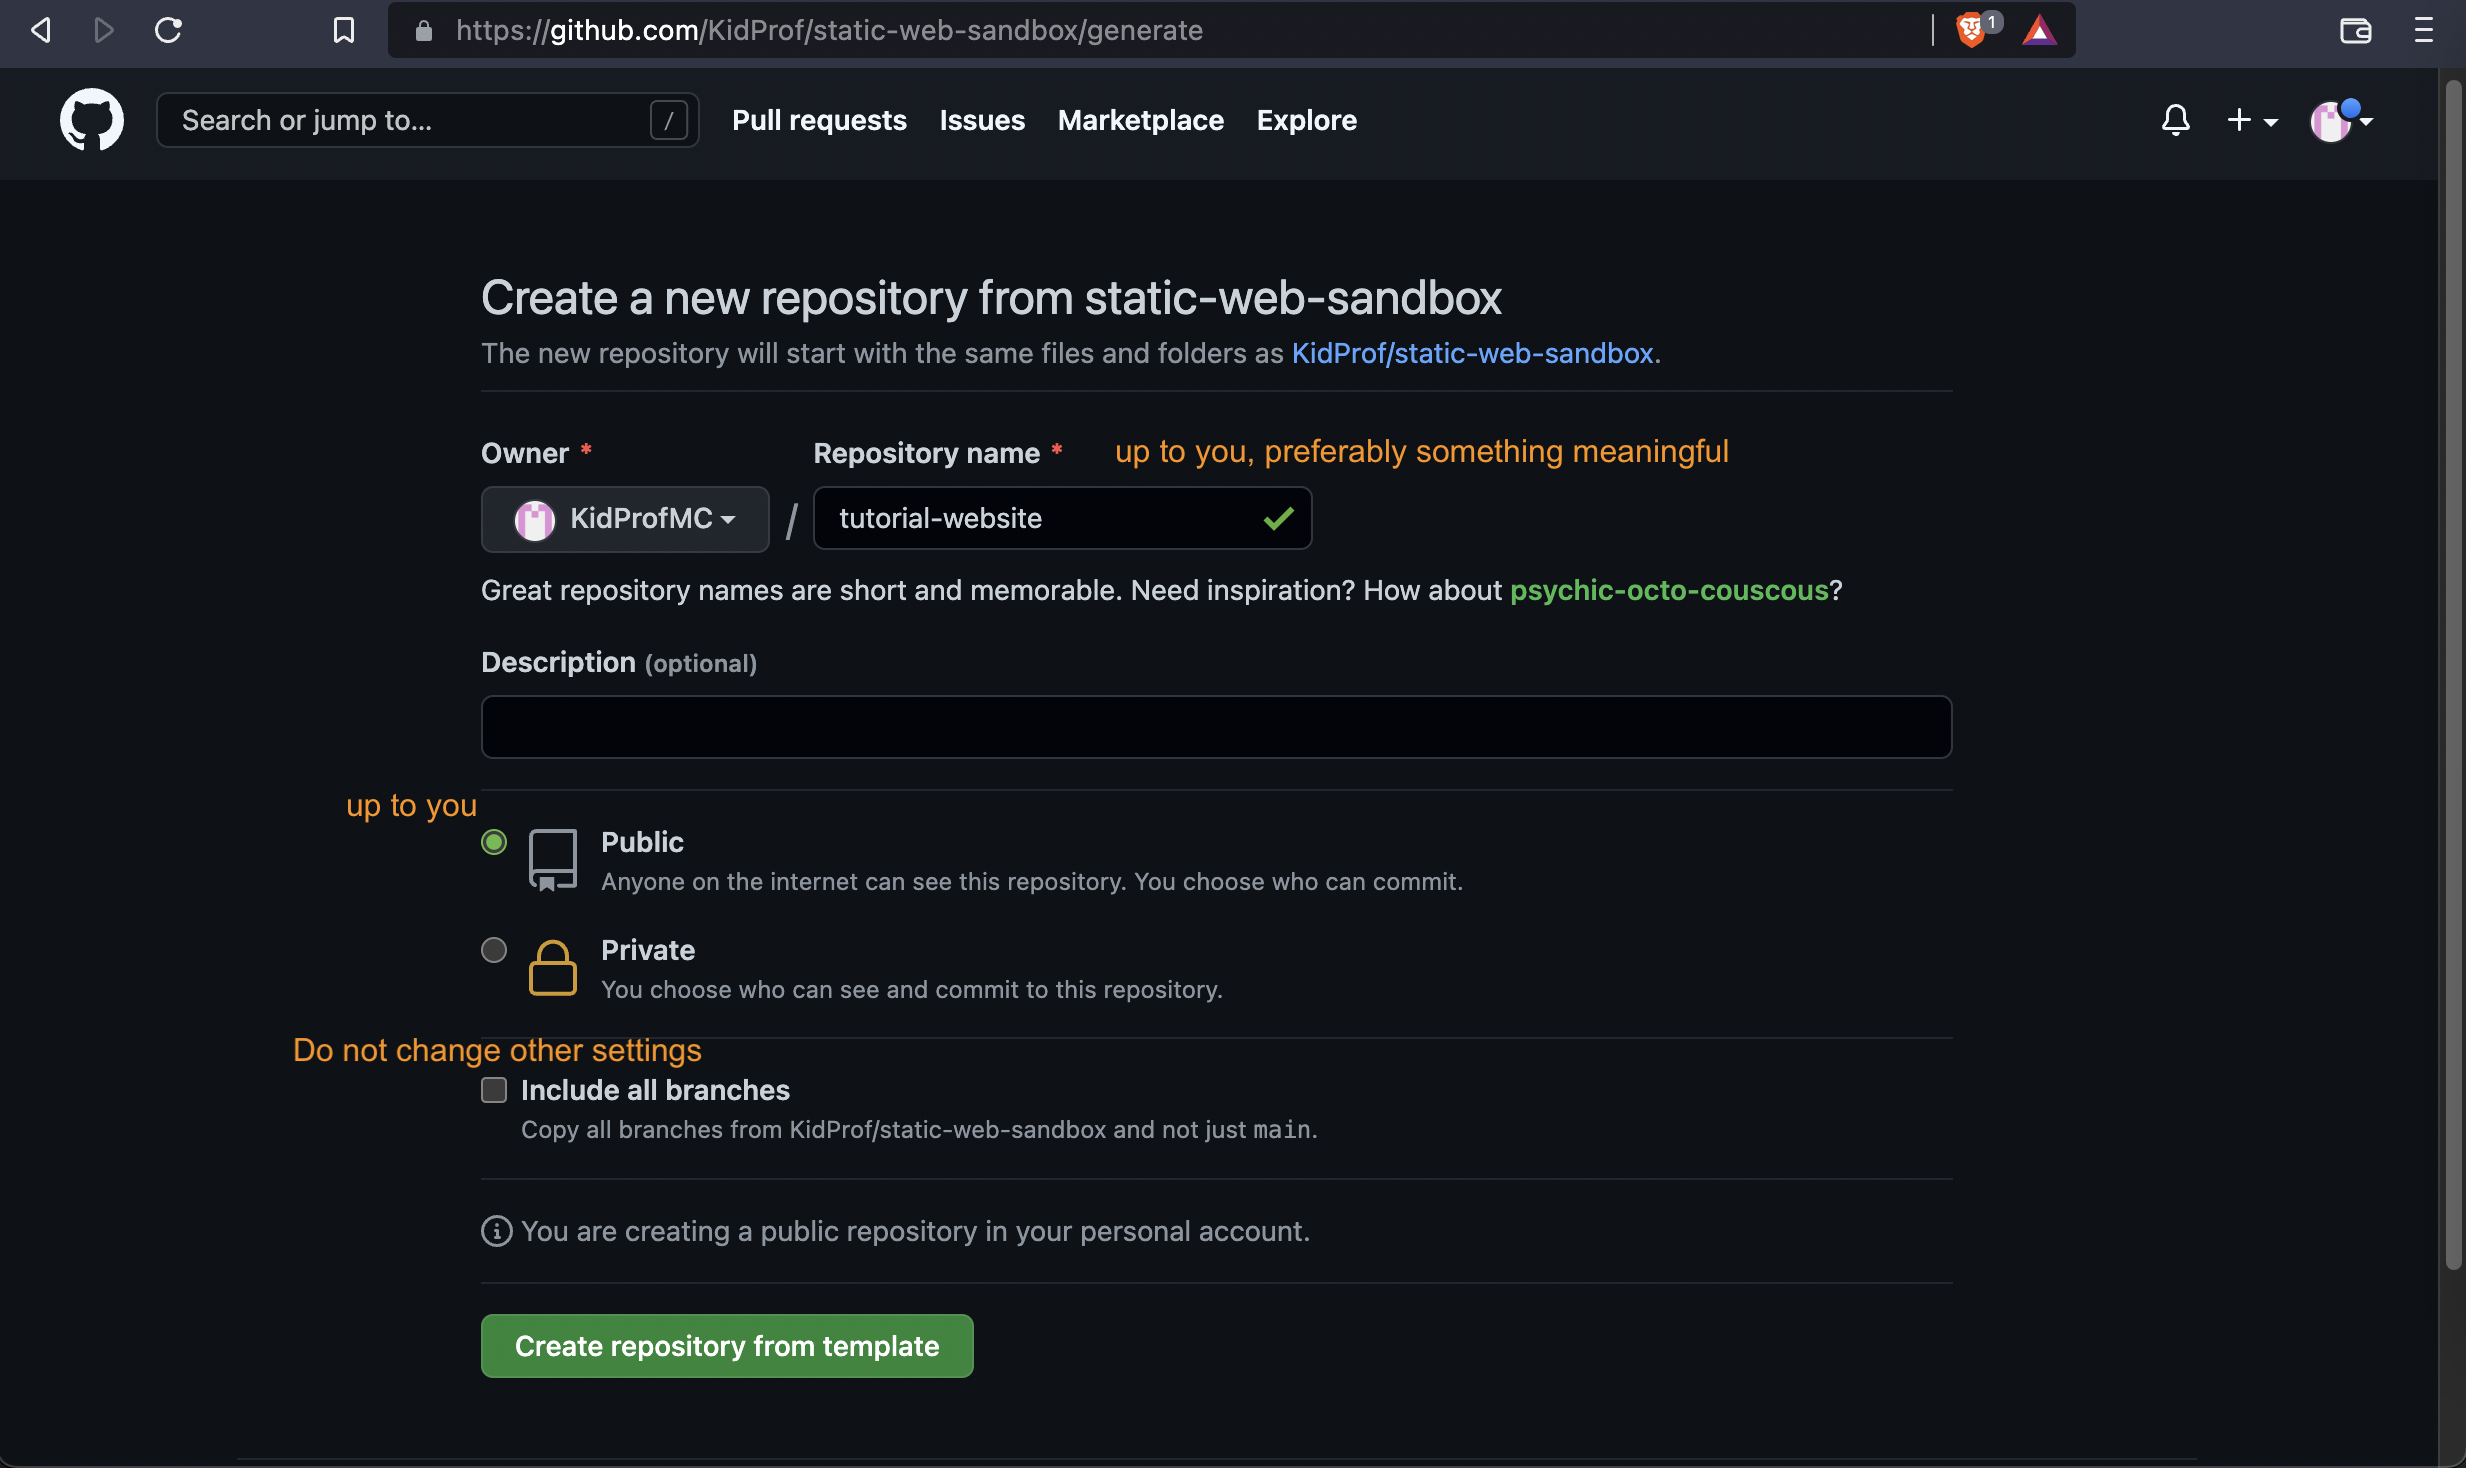
\includegraphics[width=15cm]{images/ch1-create-new-repo.png}
\caption{Creating a new repository}
\end{figure}

\section{Creating an SSH key}

An SSH key is to verify your identity on your local machine, so that you can access and manage your repositories on GitHub from your local machine.

Follow \href{https://docs.github.com/en/authentication/connecting-to-github-with-ssh/generating-a-new-ssh-key-and-adding-it-to-the-ssh-agent}{this tutorial}\footnote{Link: \url{https://docs.github.com/en/authentication/connecting-to-github-with-ssh/generating-a-new-ssh-key-and-adding-it-to-the-ssh-agent}}, then \href{https://docs.github.com/en/authentication/connecting-to-github-with-ssh/adding-a-new-ssh-key-to-your-github-account}{this tutorial}\footnote{Link: \url{https://docs.github.com/en/authentication/connecting-to-github-with-ssh/adding-a-new-ssh-key-to-your-github-account}}, and you are good to go. 
\vspace{6mm}

Use Git Bash if you are on a Windows machine, use the Terminal if you are on a MacOS or Linux machine. There is no need to understand and remember the commands, copying and pasting is one of the skills needed to be a good programmer. \textbf{The \$ symbol indicates the start of a command, so you do not need to copy the \$ symbol.}
\vspace{6mm}

For example, if I am using a Windows machine, I would run the following set of commands in my Git Bash line by line. Remember replace the email with your own email used to register for the GitHub account!

\begin{lstlisting}[language=bash]
$ ssh-keygen -t ed25519 -C "your_email@example.com"
$ eval "$(ssh-agent -s)"
$ ssh-add ~/.ssh/id_ed25519
$ clip < ~/.ssh/id_ed25519.pub
\end{lstlisting}

Then paste the SSH public key to the appropriate spot on the GitHub website according to the tutorials.

\section{Creating a folder using command line}
\label{sec:install5}

From now on, I would use the term \textbf{command line} to refer to Git Bash if you are on a Windows machine, and the Terminal if you are on a MacOS or Linux machine. 

So now open the command line, use \texttt{mkdir} followed by a folder name to create a new folder to store your code. Then, use \texttt{cd} followed by the folder name to enter to that folder.

\begin{lstlisting}[language=bash]
# KidProf in ~
$ mkdir code

# KidProf in ~
$ cd code

# KidProf in ~/code
$ 
\end{lstlisting}

\section{Downloading the code using SSH key}

Go back to your project on GitHub, click the big green button \textit{Code}, then remember to select \texttt{SSH}, then copy the URL given.

\begin{figure}[h]
\centering
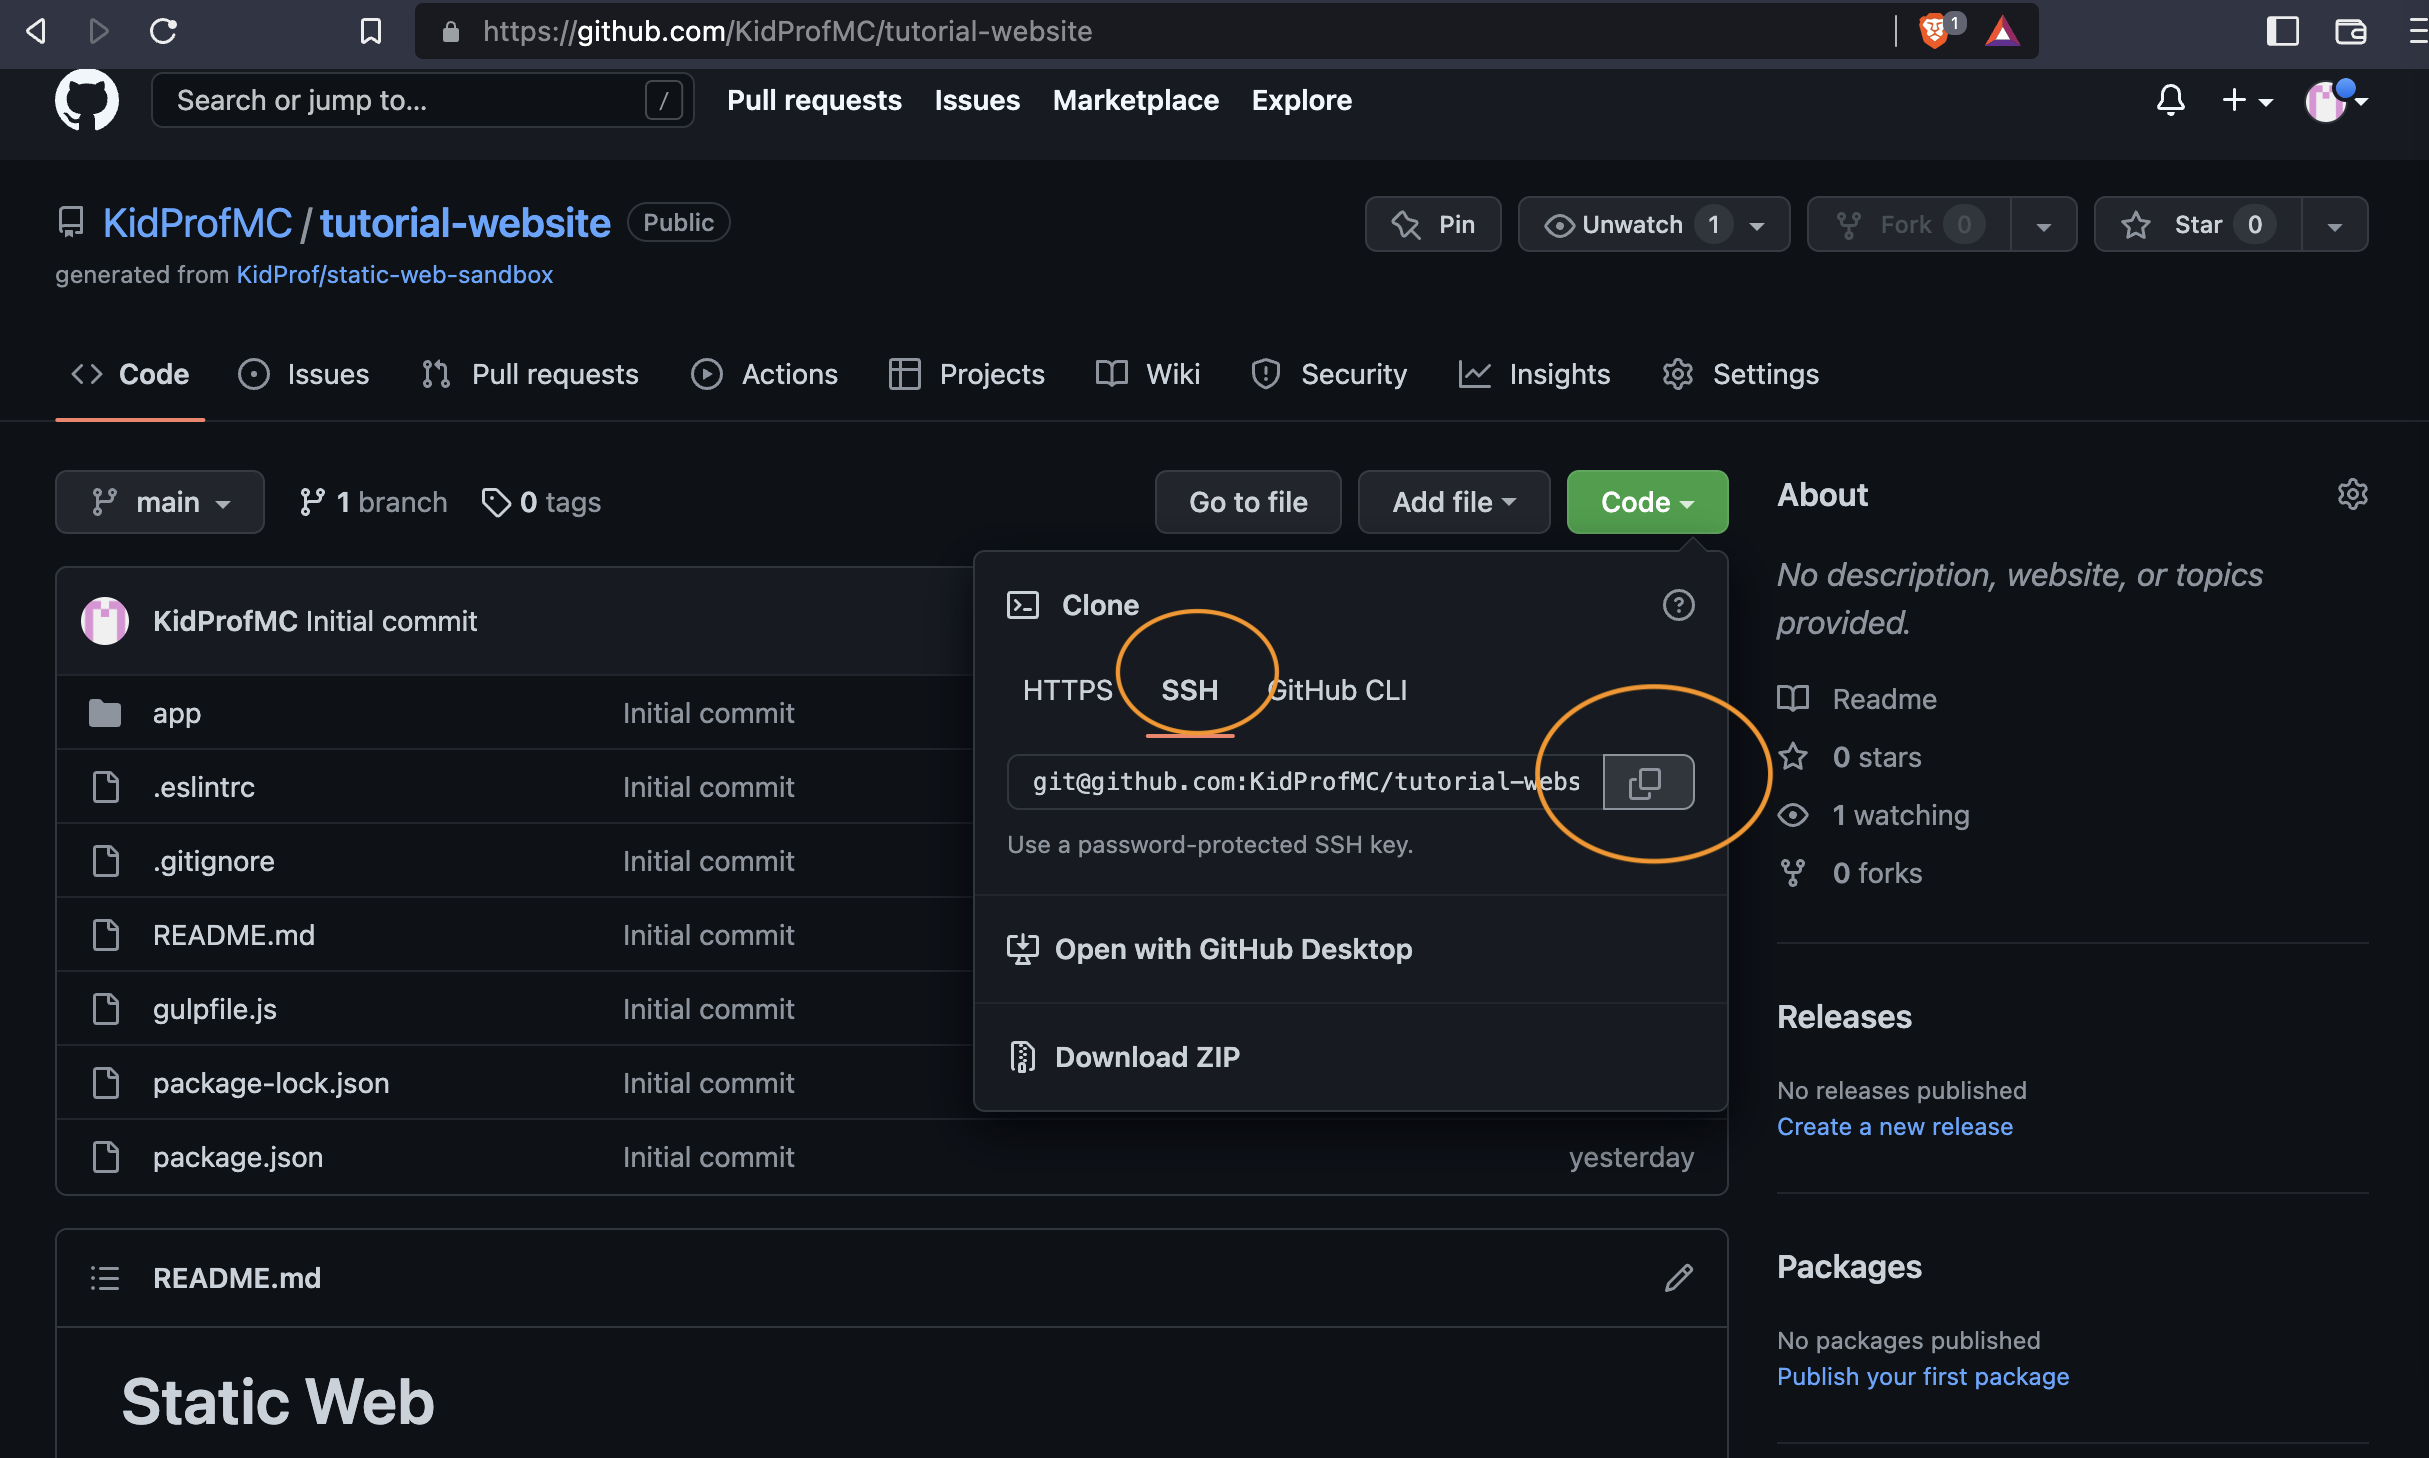
\includegraphics[width=15cm]{images/ch1-git-clone.png}
\caption{Getting the URL to download your project}
\end{figure}

Use \texttt{git clone}, followed by pasting the URL obtained from GitHub. You should use your mouse to paste the URL in the classic way, as \texttt{ctrl+V} would not work.

\section{Installing node.js}
\label{sec:install7}

Download node.js by following \href{https://nodejs.org/en/}{this link}.\footnote{Link: \url{https://nodejs.org/en/}} It should be straightforward. You should download the LTS\footnote{stands for long term support} version.

After installing, you can try running \texttt{node --version} in the command line.

\begin{lstlisting}[language=bash]
# If node is installed, it will show you the version number.
$ node --version
v16.14.0

# If node is not installed, it will show you an error message
$ node --version
zsh: command not found: node
\end{lstlisting}

\section{Installing dependencies for the project}

Open your command line, \texttt{cd} into the folder with the code in, run \texttt{npm install}. A new folder called \texttt{node\textunderscore modules} will be automatically created, with everything you need to use this project installed within that folder.

\begin{lstlisting}[language=bash]
# KidProf in ~
$ cd code

# KidProf in ~/code
$ cd tutorial-website

# KidProf in ~/code/tutorial-website
$ npm install
\end{lstlisting}

\section{Opening the web page}

Run \texttt{npm run build} to build the web page, more on this would be explained in \cref{sec:projstructure}.

Then, open the folder containing the project in file explorer/ finder. Go to the \texttt{docs} folder, open \texttt{index.html} using a web browser of your choice.

If you are unsure where your code is located, try running \texttt{pwd} in your command line, that should show you the full path that your code should be in.

\begin{lstlisting}[language=bash]
# KidProf in ~/code/tutorial-website on git:main 
$ npm run build

> static-web-sandbox@2.0.0 build
> gulp build

[09:56:22] Using gulpfile ~/code/tutorial-website/gulpfile.js
[09:56:22] Starting 'build'...
[09:56:22] Starting 'js'...
[09:56:22] Finished 'js' after 38 ms
[09:56:22] Starting 'pug'...
[09:56:22] Finished 'pug' after 83 ms
[09:56:22] Starting 'styling'...
[09:56:22] Finished 'styling' after 37 ms
[09:56:22] Starting 'imagecopy'...
[09:56:22] Finished 'imagecopy' after 2.67 ms
[09:56:22] Starting 'fontcopy'...
[09:56:22] Finished 'fontcopy' after 1.42 ms
[09:56:22] Finished 'build' after 164 ms

# KidProf in ~/code/tutorial-website on git:main 
$ pwd
/Users/KidProf/code/tutorial-website
\end{lstlisting}

\begin{figure}[h]
\centering
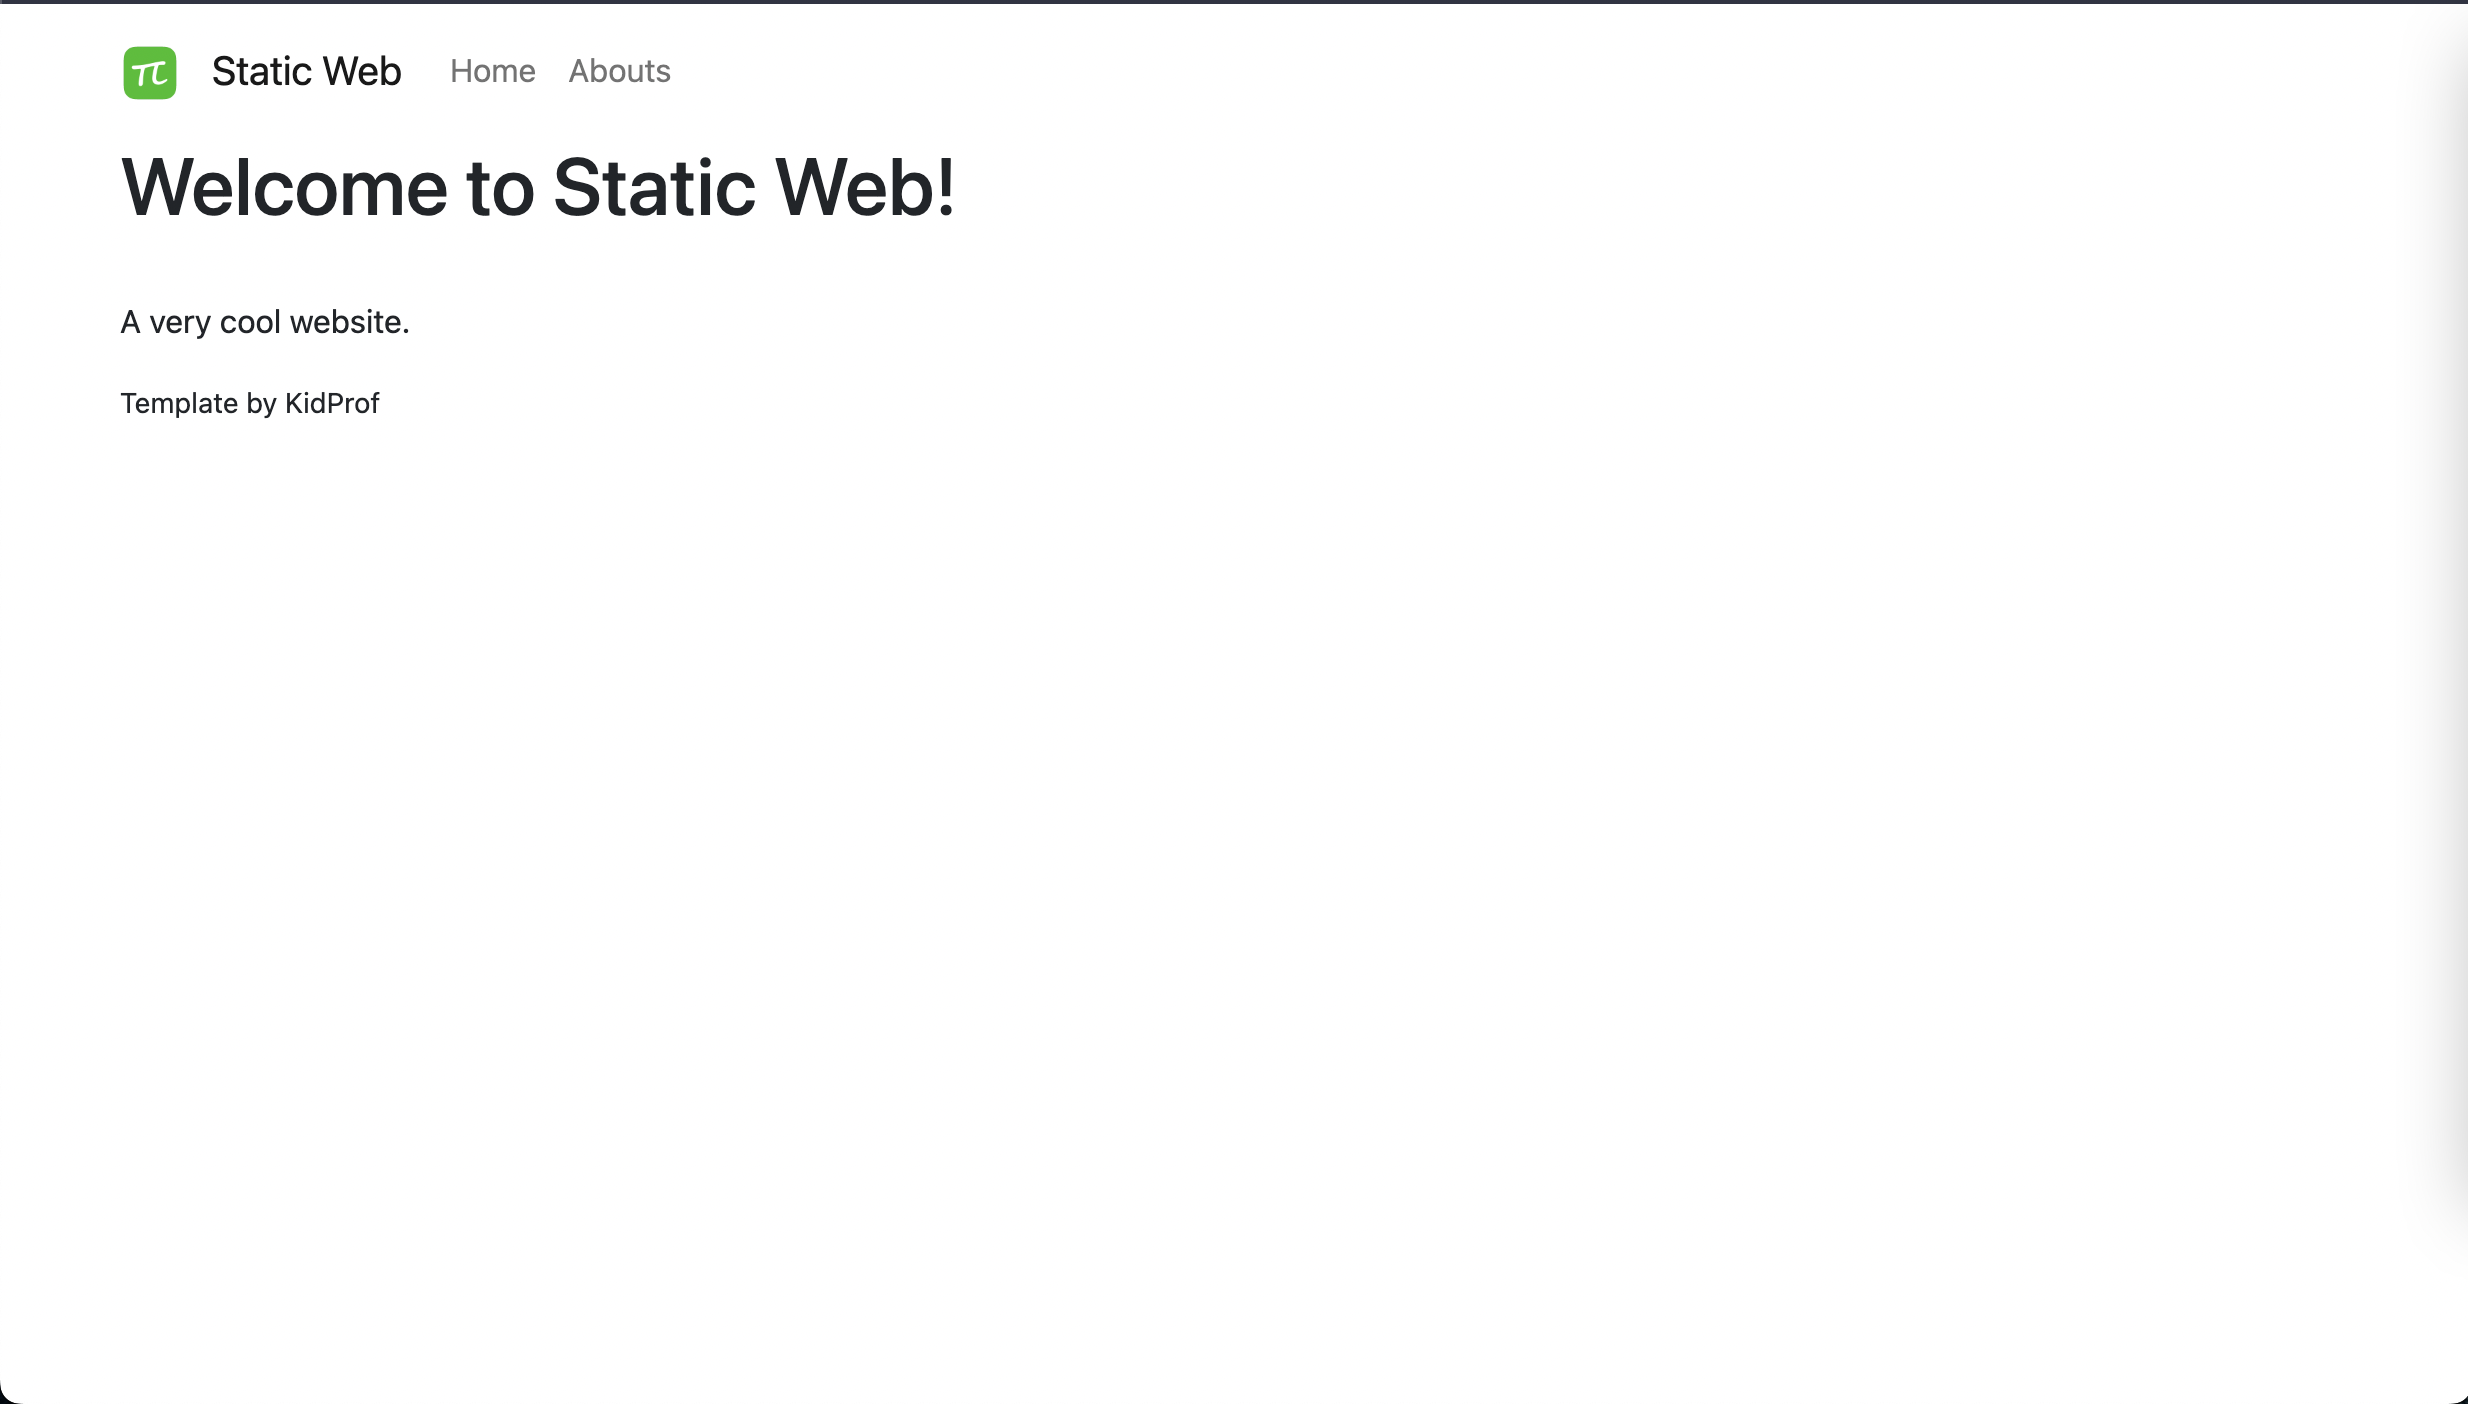
\includegraphics[width=15cm]{images/ch1-indexhtml.png}
\caption{What index.html should look like}
\end{figure}


\section{Installing VS Code}

Visual Studio Code (VS Code) is a text editor, with highlighted syntax and many more user-friendly features for you to code efficiently.

Download VS Code by following \href{https://code.visualstudio.com/}{this link}.\footnote{Link: \url{https://code.visualstudio.com/}} It should be straightforward.

\label{sec:pwdch1}
Then, open VS Code and open the folder containing the code. If you are unsure where your code is located, try running \texttt{pwd} in your command line, that should show you the full path that your code should be in.

There are a number of extensions available in VS Code, but I think they are not necessary for beginners.
\vspace{6mm}

This marks the end of the installation marathon. I hope you have learned some basic command line commands along the way, we will formally introduce them in \hyperref[sec:cmd]{the next chapter.}

\chapter{Pug.js}
\label{sec:pug1}
% Old Ch. 5

Now we have understood how the project works, let's finally write some code.
Pug.js (abbreviated as Pug) files are translated into HTML files, they provide the basic structure of the web page. Now let's learn how to write our own web page using Pug.

\section*{Further Resources (Ch 2)}

I didn't have this piece of notes back when I first learned Pug. Here is \href{https://youtu.be/kt3cEjjkCZA}{the video}\footnote{Link: \url{https://youtu.be/kt3cEjjkCZA}{the video}} that I used to learn the basics. 

You could refer to the \href{https://www.w3schools.com/tags/default.asp}{w3schools documentation}\footnote{Link: \url{https://www.w3schools.com/tags/default.asp}} to learn how to use some more tags. There is no need to understand all the tags, , but I found the ones listed more useful than the rest. The common ones are either explained in detail in this piece of notes here. There are also more like, but unfortunately we don't have time to cover them here. The translation to Pug is well described in other parts of this chapter already.

\section{How to experiment on my code?}
\subsection*{Magic on the Pug.js website}

\textit{This method is useful when you would like to check what is the HTML code generated with the Pug code you supplied, but it cannot let you visualise the elements and see how they would actually look like in the browser.}
\vspace{6mm}

The \href{{https://pugjs.org/}}{Pug.js official website}\footnote{Link: \url{https://pugjs.org/}} contains a detailed documentation on how it is translated to HTML.

What's more valuable is its interactive translator, you can just type any Pug code on any page in the documentation, \href{https://pugjs.org/language/attributes.html}{like this one}\footnote{Link: \url{https://pugjs.org/language/attributes.html}}, type Pug code on the left box and it will translate to HTML code on the right.

\begin{figure}[h]
\centering
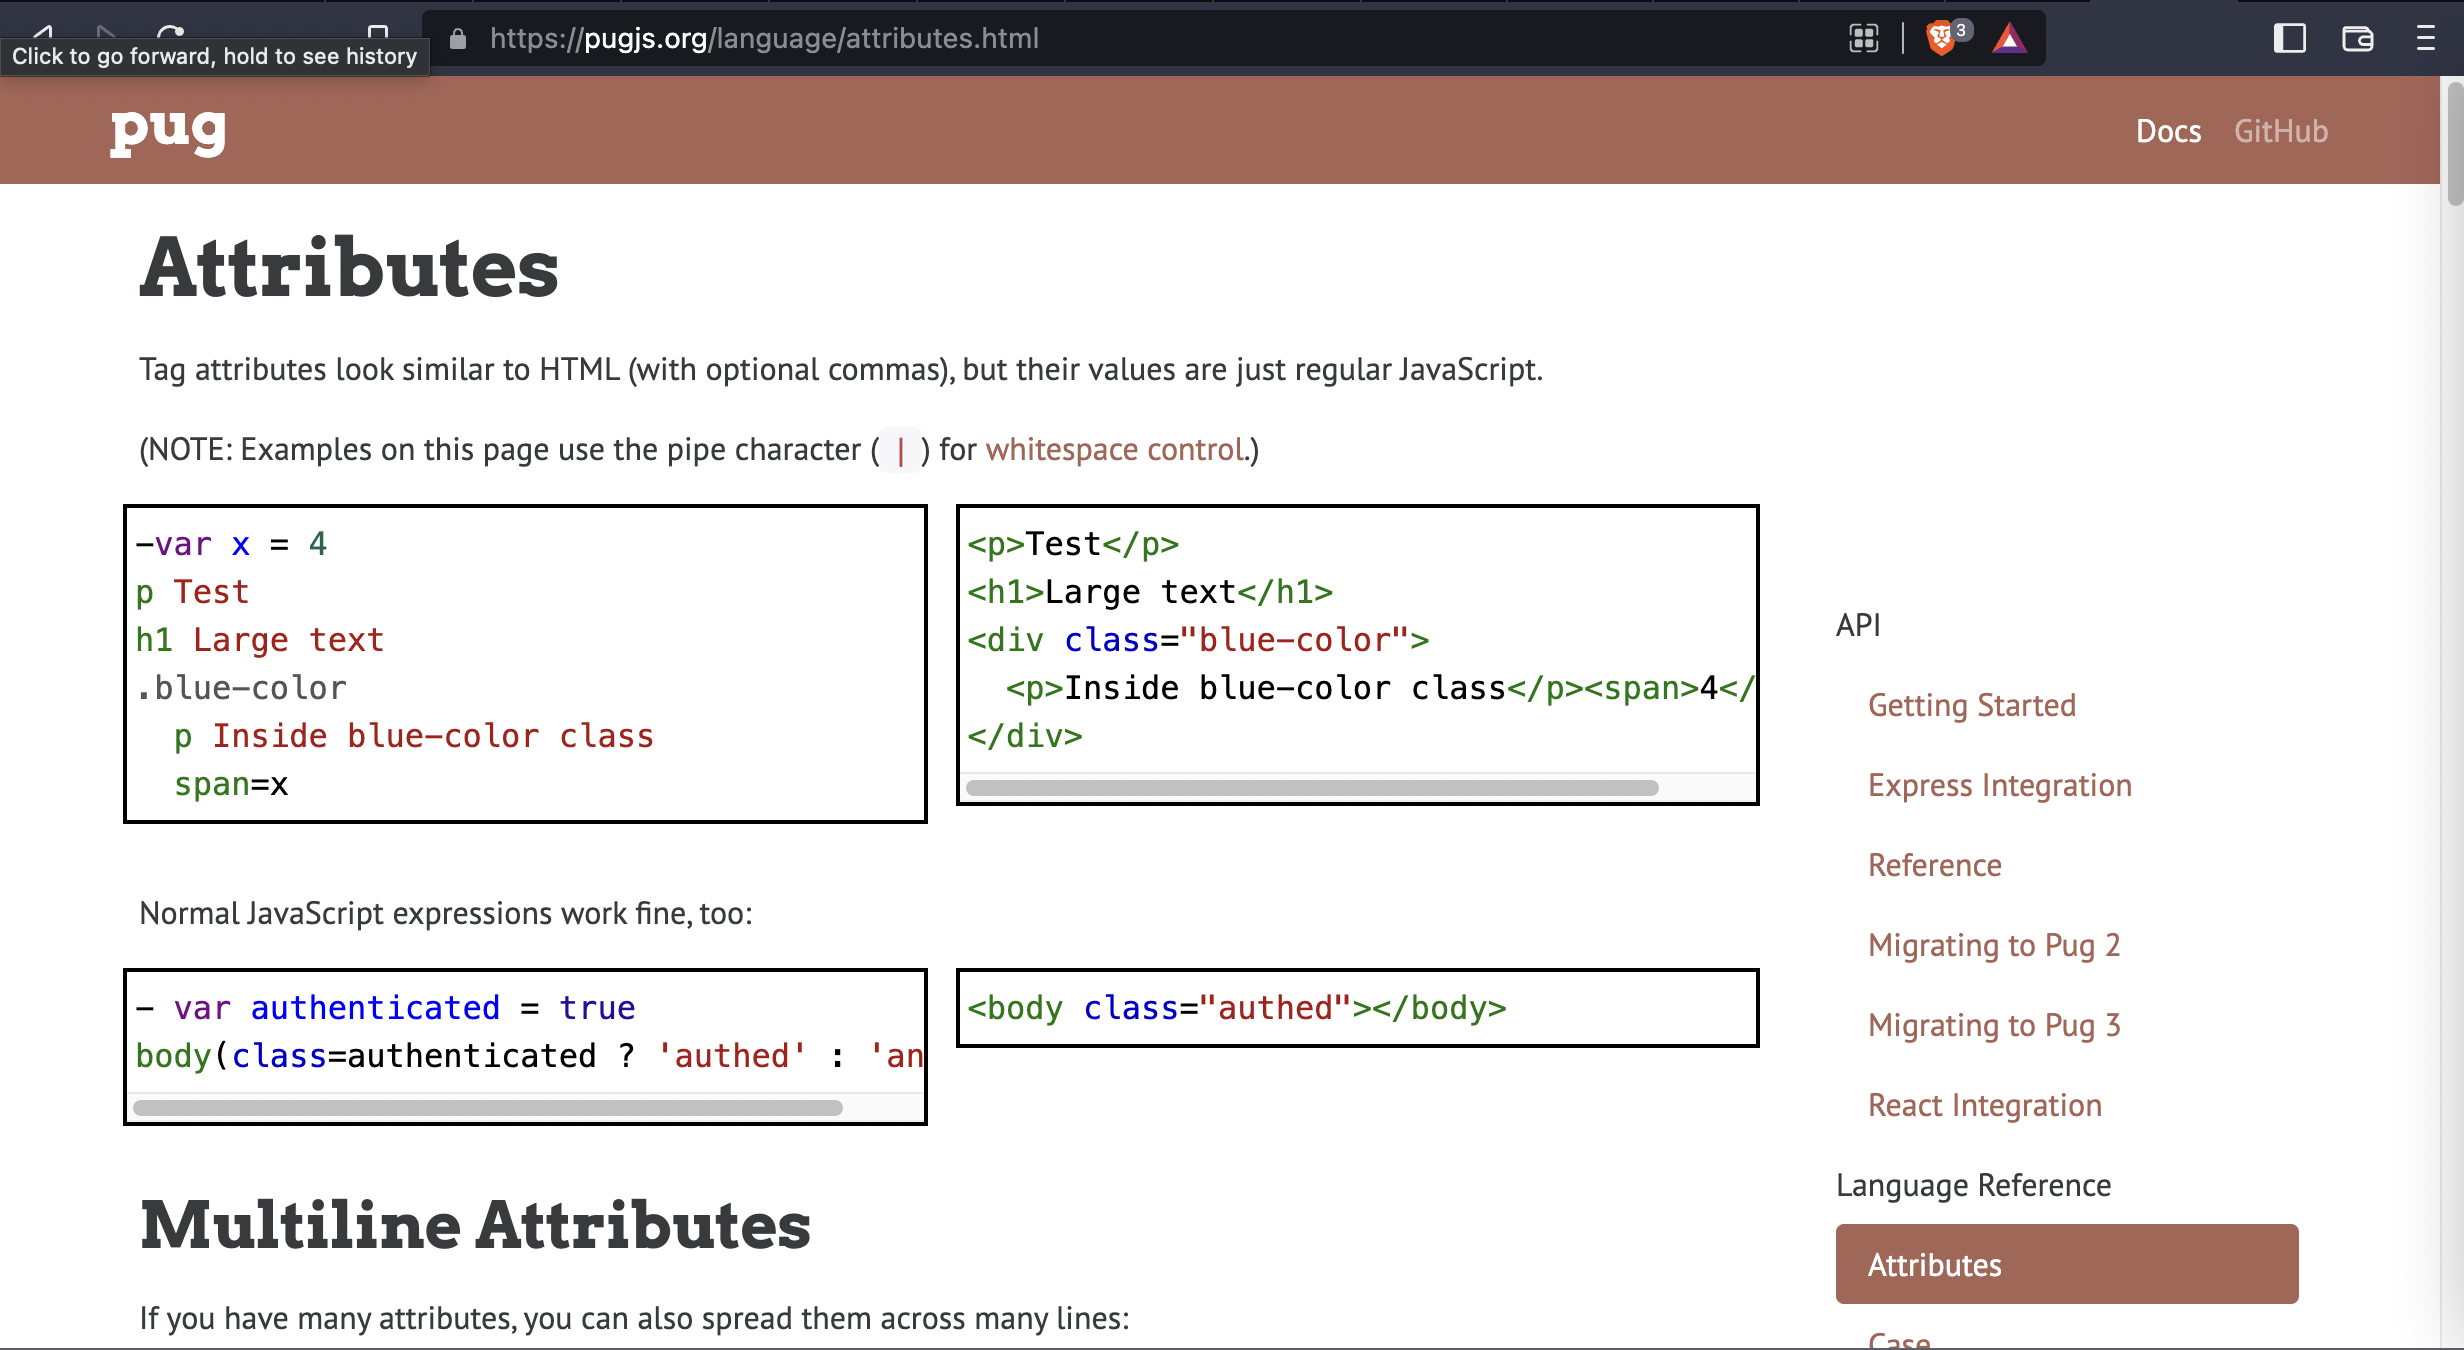
\includegraphics[width=13cm]{images/ch5-puginteractive.png}
\caption{Example usage of the interactive translator on the Pug.js official website}
\end{figure}

\subsection*{Locally on the machine}

\textit{This method is useful when you would like to visualise the elements and see how they would actually look like in the browser.}

Write the majority of your Pug code inside the \texttt{.container} class in every file under \texttt{templates/views}. 

\begin{lstlisting}[language=pug]
extends ../layouts/default

block content
	.container
		//- Your code goes here...
\end{lstlisting}

The things you write here will be translated into an HTML file matching the name of the file in the \texttt{docs} folder after you have run \texttt{npm run build}. For example, if you create a new file with the above template, called \texttt{new.pug}, then the content would appear when you open \texttt{docs/new.html} with your browser. Once again, your should NOT edit anything in the \texttt{docs} folder.

\section{General form of a Pug tag}

\begin{lstlisting}[language=pug]
a#id.class-1.class-2(href="abouts.html") Click for abouts page
\end{lstlisting}

Each line of Pug code can be divided into four sections.

\begin{enumerate}
    \item \textbf{Tag}: Specifies the type of element, can be one of the tags in the above table. The first word of the whole line would be regarded as the tag automatically by Pug.
    \item \textbf{Classes and IDs}: Give the element a reference, used in styling. We will discuss more in \cref{sec:classesids}.
    \item \textbf{Attributes}: Provides additional information for that element, in the example above, we have the \texttt{href} attribute, which tells the link to go to when we click on that element. Attributes are surrounded in parenthesis and put right after the tag, and we define them in the form of \texttt{name=value} pairs.
    \item \textbf{Plain text}: The text shown in that element. The rest of the whole line except the first word and the parenthesis following the first word.
\end{enumerate}

Classes and IDs are optional. Attributes are not needed for some of the tags. (e.g. \texttt{h1}) Plain text is not needed for some tags as well (e.g. \texttt{img}). You will see more examples along the way.

\section{Tags}

Some of you haven't coded in HTML before, so here is a quick walk-through to the basic tags, but using Pug.js syntax. Tags are like the basic building blocks of the web page, different tags corresponds to different kinds of things you can see on the web page. For example, a \texttt{p} tag denotes normal text, an \texttt{img} tag denotes an image. 
\vspace{6mm}

For those of you who have used HTML before, mind the syntactical difference, a summary of the differences will be provided in \cref{sec:pugvshtml}. 

\pagebreak

\begin{table}[H]
    \centering
    \begin{tabular}{|m{3.5em}|m{4.5em}|m{12em}|m{13em}|}
        \hline
        \textbf{Tag} & 
        Stands for &    
        Description & 
        Example in Pug
        \\ \hline \hline
        
        \texttt{p} &
        Paragraph & 
        Use this for normal text. &
        \texttt{\textbf{p} Hello world}
        \\ \hline
        
        \texttt{br} &
        Line Break & 
        Next line. e.g. to separate text into a few lines. (\cref{sec:br}) &
        \texttt{\textbf{p} this is a line \textbf{<br />} this is another line}
        \\ \hline
        
        \makecell[lb]{
            \texttt{h1}, \texttt{h2},\\ \texttt{h3}, \texttt{h4},\\ \texttt{h5}, \texttt{h6}
        } &
        \makecell[lb]{
        Header \\ 1-6 
        } & 
        Use this for titles and subheadings. \texttt{h1} is the largest, followed by \texttt{h2} and so on. &
        \makecell[lb]{
            \texttt{\textbf{h1} Header 1} \\
            \texttt{\textbf{h2} Header 2} \\
            \texttt{\textbf{h3} Header 3} \\
            ...
        }
        \\ \hline
        
        \texttt{img} &
        Image & 
        You need to specify the source \texttt{src} of the image using \textbf{attributes} (see next session). Please make sure you add your images in the \texttt{app/images} folder. (\cref{sec:img}) &
        \texttt{\textbf{img}(src="images/ bookofnumbers.jpg")}
        \\ \hline
        
        \texttt{a} &
        Anchor/ Link &
        Use this to create hyperlinks to other websites or other parts of your own website. It requires an \texttt{href} attribute indicating the destination. &
        \makecell[lb]{
            \texttt{\textbf{a}(href="abouts.html")}\\\texttt{Click for abouts page.} \\
            \texttt{\textbf{a}(href="https://www}\\\texttt{.google.com") Click}\\\texttt{for Google}
        }
        \\ \hline
        
        \makecell[lb]{
            \texttt{ul},\\\\ \texttt{ol},\\\\ \texttt{li}
        } &
        \makecell[lb]{
            unordered \\ list,\\ ordered \\ list,\\ list item
        } &
        Lists with bullet points (\texttt{ul}) or numbering (\texttt{ol}) (\cref{sec:list}) &
        \makecell[lb]{
            \texttt{\textbf{ul}} \\
            \texttt{\hspace{6mm}\textbf{li} apple} \\
            \texttt{\hspace{6mm}\textbf{li} orange} \\
            \texttt{\hspace{6mm}\textbf{li} pear} 
        }
        \\ \hline
        
        \texttt{div} &
        Division &
        It serves no purposes in adding content to the web page, but it can be used to improve organisation of your code, and it is crucial for styling. (\cref{sec:classesids}) &
        \makecell[lb]{
            \texttt{\textbf{div}} \\
            \texttt{\hspace{6mm}\textbf{h3} Numbers are} \\\texttt{\hspace{6mm}\hspace{6mm}beautiful} \\
            \texttt{\hspace{6mm}\textbf{p} - KidProf} 
        }
        \\ \hline
        
        \texttt{//-} &
        Comment &
        \tablefootnote{An alternative is \texttt{//}, using \texttt{//} means that the generated HTML file would also contain that comment, while using \texttt{//-} won't.} &
        \texttt{//- a comment} 
        \\ \hline
        
        
    \end{tabular}
\end{table}

\pagebreak

\section{Attributes}
\label{sec:img}

\textbf{Attributes} provides additional information for that element, they are surrounded in parenthesis and put right after the tag, and we define them in the form of \texttt{name=value} pairs.

Some attributes are necessary for the tags to work properly. For example, the \texttt{src} attribute that tells the \texttt{img} tag where the source of the image is. Please make sure you add your images in the \texttt{app/images} folder.
\vspace{6mm}

\begin{lstlisting}[language=pug]
img(src="images/bookofnumbers.jpg")
\end{lstlisting}

You can have more than one attributes. For example, you can specify its width and height in pixels, and also an alt text when the image cannot show properly for whatever reason.

\begin{lstlisting}[language=pug]
//- app/templates/partials/navbar.pug
img(src="images/pi-green.png" width=30 height=30 alt="pi logo")
\end{lstlisting}

However, specifying image dimensions using pixels is usually not desired because we want the image to scale based on screen width. (see \cref{sec:width}) Nonetheless, the size of the pi logo on the top left corner of the website is set using this method.
Pug uses indentation to indicate that something is in a tag

\section{How are tags put together in Pug?}

We use indentation to indicate how elements are nested. The indented tags will be surrounded by the outer tags when they got translated to HTML. We will look into some examples and also explain some of the tags in detail. 

\subsection*{Lists}
\label{sec:list}

We surround all contents of a list within a \texttt{ul} or a \texttt{ol} tag. We use \texttt{ul} (unordered list) when we need bullet points, while we use \texttt{ol} (ordered list) when we need numbering. Each bullet point is demoted by \texttt{li} (list element).

The "surrounding" I mentioned is achieved by indenting all \texttt{li} tags within the \texttt{ul} or \texttt{ol} tags.
\vspace{6mm}

\begin{lstlisting}[language=pug]
//- use of ul in the abouts page
h2 About our reference book:
ul
    li Book name: The Book of Numbers
    li Author: Tim Glynne-Jones
    li Publisher: Arcturus Publishing Limited
    li Project name: "Numbers are Fun!"
    li Topics chosen: 9, 11, 30, 365.25
    
//- A random example on the use of ol
p When you got an error message you should:
ol
    li Copy the error message
    li Go to <a href="https://www.google.com"> Google</a>
    //- The syntax used for the a tag will be discussed in the br tag section.
    li Paste and search for the error message
    li Click on the first stack overflow result
    li Copy and paste the solution
\end{lstlisting}

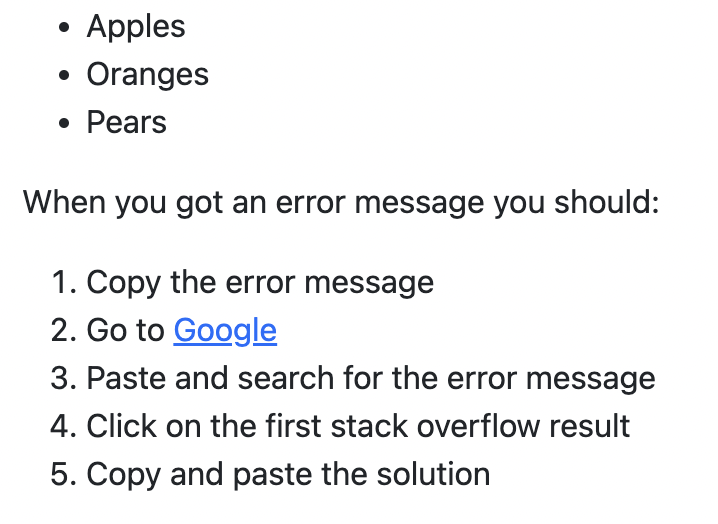
\includegraphics[width=10cm]{images/ch5-ulol.png}

\subsection*{Changing the default behaviour}

Remember that the first word in each line would be regarded as a tag. But you sometimes don't want that. 
\vspace{6mm}

For example, you might want to split the text of a \texttt{p} tag into multiple lines when the text is too long. You can actually put a \texttt{.} after the tag, and it now regards what indented within the tag as text.

\begin{lstlisting}[language=pug]
p.
	Hello, I am KidProf.
	I am a university student studying Computer Science.
	I like coding.
\end{lstlisting}


\includegraphics[width=15cm]{images/ch5-textinaline.png}

\subsection*{\texttt{br} - using normal HTML syntax in Pug}
\label{sec:br}

But when you look at the output, they are all on the same line. This is because the line breaks you made in the code is independent of the line breaks shown on the web page, \textbf{you need to explicitly use \texttt{br} tags for line breaks}. Because we are inside the \texttt{p} tag, Pug regards everything inside as text but not tags, but we can still use conventional HTML syntax to get around it.

\begin{lstlisting}[language=pug]
p.
	Hello, I am KidProf. <br />
	I am a university student studying <br />Computer Science.<br />
	I like coding.
\end{lstlisting}


\includegraphics[width=15cm]{images/ch5-textmultiplelines.png}

Alternatively, if you do not like that normal HTML code in your Pug code, you could do this instead and lead to the same result. But this is a lot of effort and affects code readability.

\begin{lstlisting}[language=pug]
p
	| Hello, I am KidProf.
	br
	| I am a university student studying
	br
	| Computer Science.
	br
	| I like coding.
\end{lstlisting}

The removal of the \texttt{.} after \texttt{p} indicates that what indented within are tags instead of plain text, so the \texttt{br} tags are registered. To indicate that the rest are plain text, the \texttt{|} character is used.

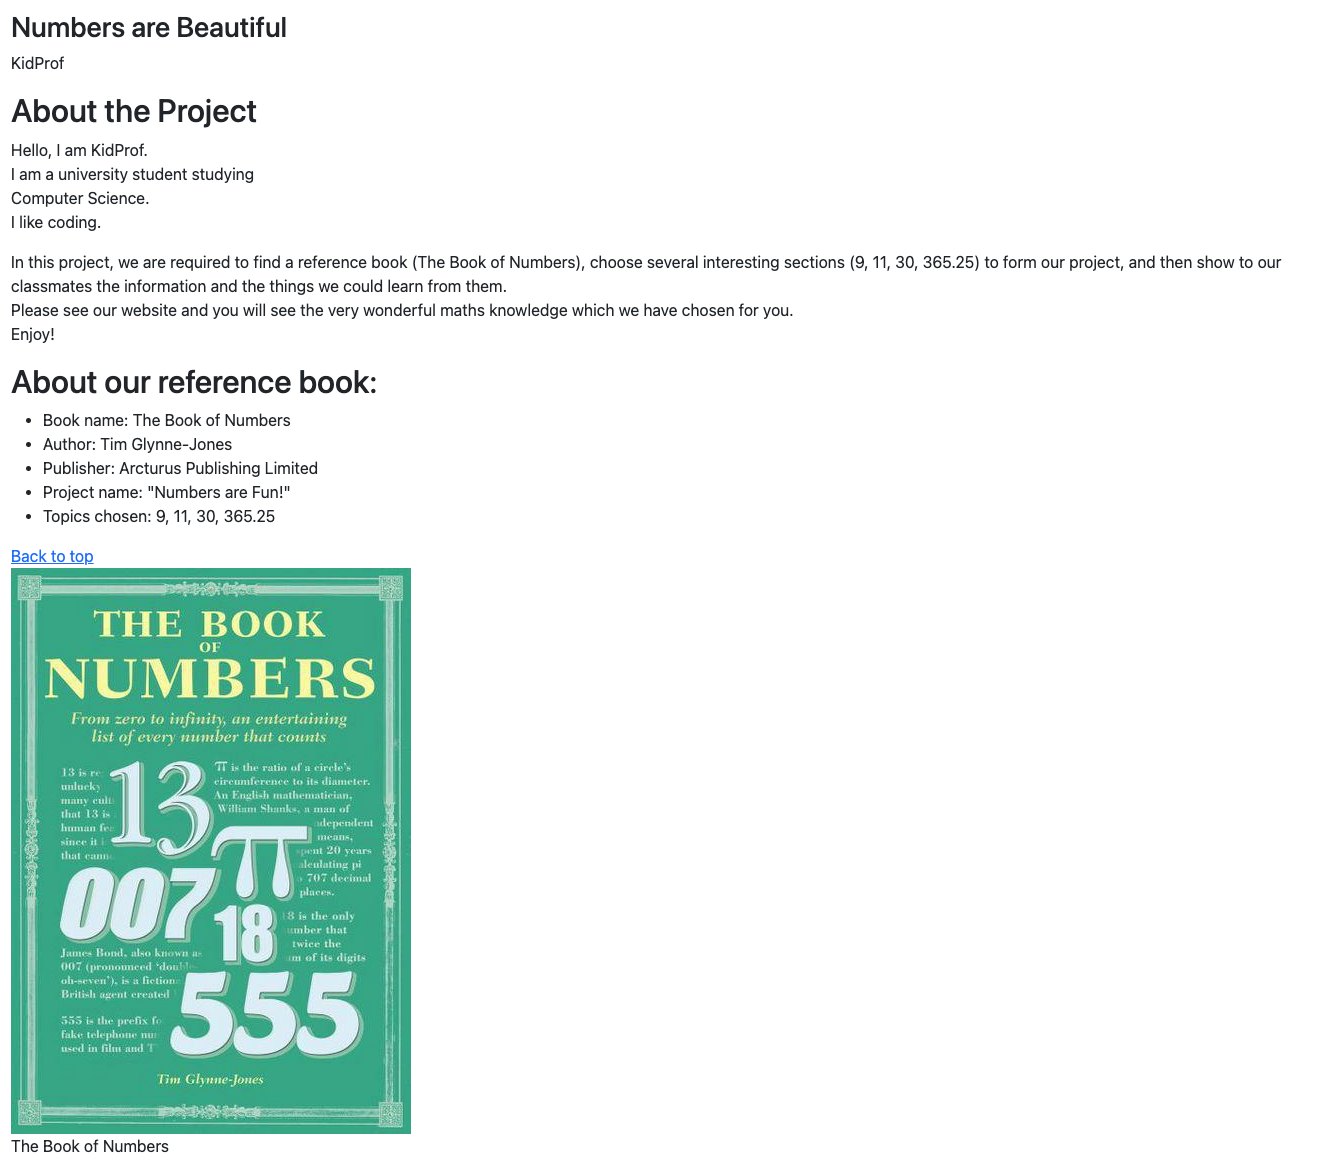
\includegraphics[width=15cm]{images/ch5-finalproduct.png}

\section{Classes and IDs}
\label{sec:classesids}

We need the notion of classes and IDs to do styling in \cref{sec:styling}, so that we can reference elements that we would like to style from the styling files.

We use \texttt{\#} followed by text to indicate an ID, and we use \texttt{.} followed by text to indicate a class. ID and class names must not contain spaces, it is a convention to either use camelCase or hyphens in place of spaces.
\vspace{6mm}

\begin{lstlisting}[language=pug]
//- templates/views/abouts.pug
div#quote
    h3 Numbers are Beautiful
    p KidProf
div#project-intro
    h2 About the Project
    p.
	    Hello, I am KidProf. <br />
	    I am a university student studying <br />Computer Science.<br />
	    I like coding.
    p.
        In this project, we are required to find a reference book (The Book of Numbers), choose several interesting sections (9, 11, 30, 365.25) to form our project, and then show to our classmates the information and the things we could learn from them. <br />
        Please see our website and you will see the very wonderful maths knowledge which we have chosen for you. <br />
        Enjoy!
h2 About our reference book:
div
    ul
        li.large-text Book name: The Book of Numbers
        li Author: Tim Glynne-Jones
        li Publisher: Arcturus Publishing Limited
        li.large-text Project name: "Numbers are Fun!"
        li.large-text.blue-text Topics chosen: 9, 11, 30, 365.25
    a(href="#self-intro") Back to top
div
    img#bookofnumbers(src="images/bookofnumbers.jpg")
    p.blue-text The Book of Numbers
\end{lstlisting}

In the code above we have defined a few IDs, including \texttt{\#quote} and \texttt{\#project-intro}; and also a few classes, including \texttt{.blue-text} and \texttt{.large-text}. 
\vspace{6mm}

\textbf{IDs must be unique within a page, while there can be multiple elements with the same class name in the same page.} An element can have more than one class.
\vspace{6mm}

To demonstrate one of the uses of IDs, I have included a link at the bottom of the example code. When you click on it, it brings you to the start of the page (if you zoom in large enough), to the element with ID \texttt{self-intro}. This feature does not work for classes because multiple elements can have the same class name in the same page.

The use of classes and IDs would become clearer in \cref{sec:styling}. We would use the classes and IDs we have defined here to reference those elements and add styles to them.\footnote{This is not the usual order of doing things. Normally, classes and IDs are added only when you want to add styles to them}

\subsection*{Classes and IDs for \texttt{div} tags}

Because \texttt{div} tags are usually associated with classes and IDs, the keyword \texttt{div} can be omitted if you have at least one class or IDs associated with it. For example, \texttt{\#quote} is equivalent to \texttt{div\#quote}.

\begin{lstlisting}[language=pug]
//- templates/views/abouts.pug
#quote
    h3 Numbers are Beautiful
    p KidProf
#project-intro
    h2 About the Project
    ...
\end{lstlisting}

\section{Summary: Pug VS HTML syntax}
\label{sec:pugvshtml}

\textit{Skip if you have not learnt HTML before, this section aims to allow HTML programmers to relate what we are learning to what they have learnt}
\vspace{6mm}

\begin{itemize}
\item Pug uses indentation to indicate that something is in a tag while HTML uses closing tags. Each line corresponds to a single tag normally. On the other hand, indentation and next lines are not important in HTML syntax.
\vspace{6mm}

\begin{lstlisting}[language=pug]
//- pug
ul
  li A
  li B
  li C
\end{lstlisting}

\begin{lstlisting}[language=html]
<!-- HTML - poorly formatted, but would still work! -->
<ul><li>A</li><li>B</li><li>C</li></ul>
\end{lstlisting}

\item All attributes should be put within parenthesis after the tag in Pug, while attributes should be put within the opening tag in HTML.
\vspace{6mm}

\begin{lstlisting}[language=pug]
//- pug
a(href="abouts.html") Click to go to the abouts page.
\end{lstlisting}

\begin{lstlisting}[language=html]
<!-- HTML -->
<a href="abouts.html">Click to go to the abouts page.</a>
\end{lstlisting}

\item Classes and IDs declarations can be simplified with Pug using the syntax shown in \cref{sec:classesids}. The \texttt{div} keyword can also be omitted when used with classes and IDs.
\vspace{6mm}

\begin{lstlisting}[language=pug]
//- pug
a#abouts-link.class1.class2(href="abouts.html") Click to go to the abouts page.
\end{lstlisting}

\begin{lstlisting}[language=html]
<!-- HTML -->
<a href="abouts.html" id="abouts-link" class="class1 class2">Click to go to the abouts page.</a>
\end{lstlisting}

\end{itemize}
\chapter{Command Line}
\label{sec:cmd}
% Old Ch. 2

Command line is important because you can work more efficiently than using graphical interfaces if you are proficient at command line tools. And you will come across some situations where only command line is available (e.g. when accessing a remote server).

I would use the term \textbf{command line} to refer to Git Bash if you are on Windows, or the Terminal if you are on MacOS, or the Shell if you are on Linux. 

\section{Basic commands}

\textit{Covered in \href{https://www.youtube.com/watch?v=oIsH0V3fRt8&list=PLjGmdnqrOKuYXiu7lgG5HW71jPEUd1XCm&index=2}{video 1 of the series}}

\subsection{\texttt{ls}}

\texttt{ls} stands for list. Lists out the files and folders you have in your current directory. \textbf{Directory is another word for folder.}
\vspace{6mm}

\begin{lstlisting}[language=bash]
$ ls
README.md   docs  node_modules  package.json    
app     gulpfile.js     package-lock.json
\end{lstlisting}

You could run \texttt{ls -a} to show hidden files and folders as well, which are the ones with their names start with a \texttt{.}

\begin{lstlisting}[language=bash]
$ ls -a
.   .git    docs    package.json
..  .gitignore  gulpfile.js
.DS_Store   README.md   node_modules
.eslintrc   app package-lock.json
\end{lstlisting}

As you can see a hidden folder \texttt{.git} and a hidden file \texttt{.gitignore} are displayed.

\subsection{\texttt{cd}}

\texttt{cd} stands for change directory, self explanatory ;). Use \texttt{cd ..} to go back to the previous directory (to go out one folder). 
\vspace{6mm}

\begin{lstlisting}[language=bash]
# KidProf in ~
$ cd code

# KidProf in ~/code
$ cd ..

# KidProf in ~
\end{lstlisting}

\subsection{\texttt{pwd}}

\texttt{pwd} shows the current directory you are in in full. As shown in \cref{sec:pwdch1} it makes it easier for you to locate our work folder in Finder/ File Explorer.
\vspace{6mm}

\begin{lstlisting}[language=bash]
# KidProf in ~
$ pwd
/Users/KidProf
\end{lstlisting}

\subsection{\texttt{touch}}

Creates a new file. For example, \texttt{touch test.txt}

\subsection{\texttt{mkdir}}

Creates a new folder. For example, \texttt{mkdir code}
\vspace{6mm}

It is not advised to have spaces in folder and file names, but if you somehow wanted to, you have to surround the name with double quotes, for instance, \texttt{touch "file with space.txt"} and \texttt{mkdir "folder with space"}.
\subsection{\texttt{--version}}

To check the version of a certain software. It is commonly used to verify that you have installed the software correctly. 

\begin{lstlisting}[language=bash]
(node is installed)
$ node --version
v16.14.0

(node is not installed)
$ node --version
bash: command not found: node
\end{lstlisting}

\section{A word on directories}
\label{sec:dir}
\texttt{.} refers to the current directory.

\texttt{..} refers to the previous directory.
\vspace{6mm}

\texttt{$\sim$} refers to the home directory, it is the initial directory when you open the command line. In the \texttt{pwd} example, you can see the home directory of my Mac is \texttt{/Users/KidProf}. You should do most of your work inside this home directory. To go back to the home directory, do \texttt{cd $\sim$} This is useful when you get stuck in some other directories.
\vspace{6mm}

When the path is not prepended with a \texttt{/}, it is a relative path. Meaning that it is relative to the current directory.

When the path is prepended with a \texttt{/}, it is an absolute path. 

\begin{lstlisting}[language=bash]
(cd to an relative path)
# KidProf in ~
$ cd code

# KidProf in ~/code

(cd to an absolute path)
# KidProf in ~
$ cd /Users/KidProf/code

# KidProf in ~/code
\end{lstlisting}

\section{General tips}

\textit{Covered in \href{https://www.youtube.com/watch?v=oIsH0V3fRt8&list=PLjGmdnqrOKuYXiu7lgG5HW71jPEUd1XCm&index=2}{video 1 of the series}}
\vspace{6mm}

Use up and down arrow to navigate your command history. Very useful when you are calling the same command repeatedly or when you made some typos.
\vspace{6mm}

Use \texttt{tab} for auto completing file and folder names.
\vspace{6mm}

Use \texttt{ctrl+C} to terminate any process, useful when a certain process got stuck or your accidentally run something that you should not run. 
This makes it impossible to use \texttt{ctrl+C} as the copy shortcut, this also applies to cut and paste shortcuts. instead, just use your mouse. There are shortcuts specifically for git bash for these operations but I would not bother to remember them.
\vspace{6mm}

\section{More commands}
\label{sec:rmcpmv}
\textit{Advanced,}
\textit{covered in \href{https://www.youtube.com/watch?v=U0bDr7b2cOM&list=PLjGmdnqrOKuYXiu7lgG5HW71jPEUd1XCm&index=8}{video 6 of the series}}\footnote{Thank you TL;DR for the simplified documentation in this section.}

\textit{\textbf{WARNING:} It is not possible to recover removed files if you delete them through the command line, so just be slightly cautious on what you are typing.}
\vspace{6mm}

\subsection{\texttt{rm}}

\texttt{rm} stands for remove. Remove files or directories.
\vspace{6mm}

Remove a file: 

\texttt{rm path/to/file path/to/another/file}
\vspace{6mm}

Remove a directory:

\texttt{rm \textbf{-rf} path/to/directory}
\vspace{6mm}

\texttt{-r} stands for recursively, it is needed when you remove or copy directories. \texttt{-f} stands for forcibly, it is needed when you remove directories so that the command line will not prompt you again and again for confirmation.

\subsection{\texttt{cp}}

\texttt{cp} stands for copy. Copies files and directories.
\vspace{6mm}

Copy a file to another location:

\texttt{cp path/to/source\textunderscore file.ext path/to/target\textunderscore file.ext}
\vspace{6mm}

Copy a directory to another location: (again \texttt{-r} is needed\footnote{Don't ask me why \texttt{-f} is needed, but it doesn't harm if you include it anyways.})

\texttt{cp \textbf{-r} path/to/source\textunderscore directory path/to/target\textunderscore directory}

\subsection{\texttt{mv}}

\texttt{mv} stands for move. Move files and directories. It is also useful in renaming the files and directories.
\vspace{6mm}

Move a file or directory to an arbitrary location:

\texttt{mv source target}

\section{Vim - command line text editor}
\label{sec:vim}

\textit{Advanced}
\vspace{6mm}

The default text editor is called Vim. It may appear when you run some commands that require messages to be inputted, for example, \texttt{git commit} (More in \cref{sec:gcmsg}).

Unfortunately, it is quite difficult to use and needs some time to get used to. So I tried my best to provide alternative commands that prevent this text editor from popping up, for example, using \texttt{git commit -m "message"}

However, here are the basics of using Vim, so that you will not get too lost when you encounter it. You can practice by entering \texttt{vim} in the command line.

You start in a mode called "normal mode". You can’t immediately type anything.

In order to get typing press \texttt{i} (stands for insert). This will bring you to "insert mode", so named because in this mode you can actually type.

When you are done typing press \texttt{esc}. This will bring you back to "normal mode".

In order to save your work you want to type :w and press return. And in order to exit vim you want to type \texttt{:q} and press return. Because saving and quitting is a very common action, there is actually a shortcut \texttt{:x}, which stands for \texttt{:wq} (which just combines \texttt{:w} and \texttt{:q}).\footnote{Reference: \url{https://web.mit.edu/6.005/www/fa14/tutorial/git/config.html}}


If you do not wish to save the file, you can use \texttt{:q!}

\begin{table}[H]
    \centering
    \caption{Table of common command line commands}
    \vspace{6mm}
    \begin{tabular}{|m{13em}|m{22em}|}
        \hline
        \textbf{Command} & 
        Description 
        \\ \hline \hline
        
        \texttt{ls} &
        Lists out the files and folders you have in your current directory
        \\ \hline
        
        \texttt{cd $<$dir$>$} &
        Changes to the specified directory
        \\ \hline
        
        \texttt{cd ..} &
        Changes to the previous directory
        \\ \hline
        
        \texttt{cd $\sim$} &
        Changes to the root directory
        \\ \hline
        
        \texttt{pwd} &
        Shows the current directory you are in in full
        \\ \hline
        
        \texttt{touch $<$filename$>$} &
        Creates a new file
        \\ \hline
        
        \texttt{mkdir $<$dir$>$} &
        Creates a new folder
        \\ \hline
        
        \texttt{$<$software$>$ --version} &
        Checks the version of a certain software
        \\ \hline
        
        \texttt{rm $<$filename$>$} &
        Removes a file with name \texttt{$<$filename$>$}
        \\ \hline
        
        \texttt{rm -rf $<$dir$>$} &
        Removes a folder with \texttt{$<$dir$>$}
        \\ \hline
        
        \texttt{cp $<$src-file$>$ $<$destination-file$>$} &
        Copies a file from \texttt{$<$src-file$>$} to \texttt{$<$destination-file$>$}
        \\ \hline
        
        \texttt{cp -r $<$src-dir$>$ $<$destination-dir$>$} &
        Copies a folder from \texttt{$<$src-dir$>$} to \texttt{$<$destination-dir$>$}
        \\ \hline
        
        \texttt{mv $<$src$>$ $<$destination$>$} &
        Moves a file/folder from \texttt{$<$src$>$} to \texttt{$<$destination$>$}
        \\ \hline
        
    \end{tabular}
\end{table}

\chapter{Git}
\label{sec:ch3}
Git is important because it allows you to work and communicate with people using just a few simple commands. By following its rules and conventions, you can work with others efficiently, without having to send zip files back and forth through emails. It also allows version control, for you to keep track of changes you have made to your code, and revert to a previous version or take reference from your previous changes when necessary.
\vspace{6mm}

We will focus on getting Git set up and basic commands in this chapter. After reading this chapter, you will be able to use Git alone for version control, as if it is a save button of your work. A few more commands will be introduced in \cref{sec:git2} to allow you to work with others.

\begin{center}

\includegraphics[width=10cm]{images/ch0-version-control.jpeg}
\end{center}

\section{Git VS GitHub}

Before we start, it is a good idea to distinguish between Git and GitHub. Git runs on your local machine, keeping track of the changes you have made locally. While GitHub is a cloud service provider\footnote{There are also other similar cloud service provider but GitHub is the most popular one}, keeping track of changes made to different people. That version of the project on GitHub should be the one that all local machines follow.

\begin{center}
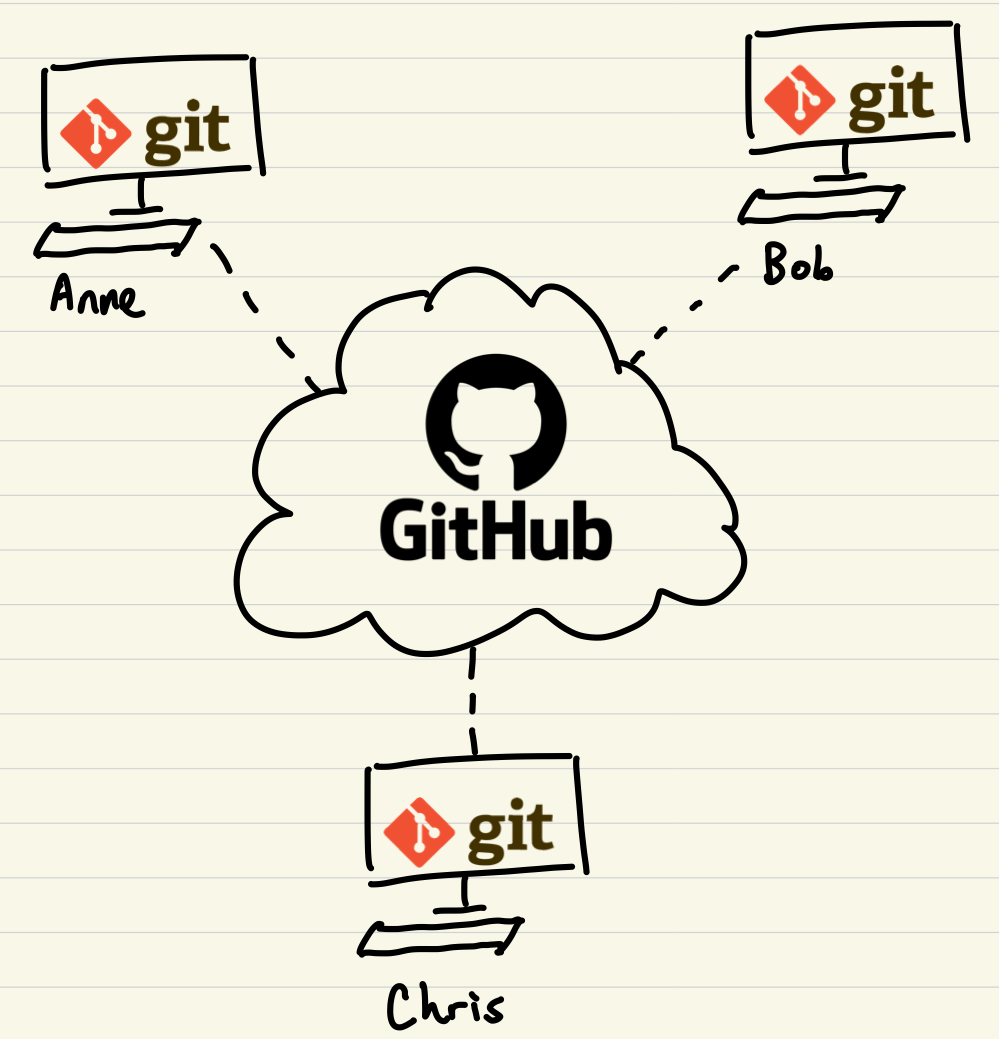
\includegraphics[width=10cm]{images/ch3-gitgithub.png}
\end{center}

\section{First time using Git}
\label{sec:gitfirst}

\textit{Covered in \href{https://www.youtube.com/watch?v=wQmFz-Ggxuo&list=PLjGmdnqrOKuYXiu7lgG5HW71jPEUd1XCm&index=4}{video 3 of the series}}
\vspace{6mm}

Let's just change out \texttt{app/templates/views/index.pug} slightly so that we can make our first push to GitHub. Or if you are working on other projects, you can pick a random file and made some edits.

\begin{lstlisting}[language=pug]
//- app/templates/views/index.pug
extends ../layouts/default

block content
	.container
		h1 Welcome to Static Web!
		br
		p A very cool website.
		p This web is made for tutorial purposes.
\end{lstlisting}

One very useful command - \texttt{git status} displays information about current situation, it might also contains some hints on which command(s) you need to run to proceed.

\begin{lstlisting}[language=bash]
$ git status
On branch main
Your branch is up to date with 'origin/main'.

Changes not staged for commit:
  (use "git add <file>..." to update what will be committed)
  (use "git restore <file>..." to discard changes in working directory)
	modified:   app/templates/views/index.pug

no changes added to commit (use "git add" and/or "git commit -a")
\end{lstlisting}

\subsection*{First add}
So you can see it is prompting you to run \texttt{git add <file>}. Instead, I would prefer \texttt{git add .} As discussed in \cref{sec:dir}, \texttt{.} refers to the current directory. That means, we are including all the changes in the folder to be ready for a commit.

\begin{lstlisting}[language=bash]
$ git add .
\end{lstlisting}

Then, run \texttt{git status} again to asset the situation. The modified file should now be highlighted in green. (sadly you cannot see the green highlighting in LaTeX)

\begin{lstlisting}[language=bash]
$ git status
On branch main
Your branch is up to date with 'origin/main'.

Changes to be committed:
  (use "git restore --staged <file>..." to unstage)
	modified:   app/templates/views/index.pug
\end{lstlisting}

\subsection*{First commit (and set up your name and email)}

Next step, we are now ready to commit. \texttt{git commit} seals and confirms your changes into one chunk, and adds a commit message. The \textbf{commit message} should be meaningful, summarising what you have achieved with these code changes.

\begin{lstlisting}[language=]
$ git commit -m "experimenting with git"
[main e7bc529] experimenting with git
Committer: KidProf <kidprof@KidProfs-MacBook-Air.local>
Your name and email addresses were configured automatically
...
git config --global --edit
git config --amend --reset-author
1 file changed, 2 insertions(+), 1 deletion(-)
\end{lstlisting}

We got a problem here, our username and email do not match with the ones on GitHub. We need to \#1) change the default name and email on our device, and \#2) change the name and email for this particular commit.

Instead of the commands recommended automatically by Git, I recommend variants of those commands which are listed below, because these commands won't trigger the command line text editor to pop up. (see \cref{sec:vim})

Run the following two commands for \#1, replace with your own ones. Surround your name with double quotes if your name contains spaces.

\begin{lstlisting}[language=bash]
$ git config --global user.name KidProf
$ git config --global user.email kidprof@gmail.com
\end{lstlisting}

To verify, rerun those two commands but without the name and email, it should display your name and email as output.

\begin{lstlisting}[language=bash]
$ git config --global user.name
KidProf
$ git config --global user.email
kidprof@gmail.com
\end{lstlisting}

This command is for \#2.

\begin{lstlisting}[language=bash]
$ git config --amend --reset-author --no-edit
\end{lstlisting}

All set, now try running \texttt{git status} again.

\begin{lstlisting}[language=]
$ git status
On branch main
Your branch is ahead of 'origin/main' by 1 commit.
  (use "git push" to publish your local commits)

nothing to commit, working tree clean
\end{lstlisting}

\subsection*{First push}

Time to run \texttt{git push}, our last step. Except it might return an error.

\begin{lstlisting}[language=]
$ git push
fatal: The current branch main has no upstream branch.
To push the current branch and set the remote as upstream, use

    git push --set-upstream origin main
\end{lstlisting}

This one is quite an easy fix, just run the substitute command as instructed. You will need this whenever you are pushing a new branch to GitHub. \texttt{git push} should be sufficient for subsequent pushes.

\begin{lstlisting}[language=]
$ git push --set-upstream origin main
Enumerating objects: 11, done.
Counting objects: 100% (11/11), done.
Delta compression using up to 8 threads
Compressing objects: 100% (6/6), done.
Writing objects: 100% (6/6), 575 bytes | 575.00 KiB/s, done.
Total 6 (delta 3), reused 0 (delta 0), pack-reused 0
remote: Resolving deltas: 100% (3/3), completed with 3 local objects.
To github.com:KidProfMC/tutorial-website.git
\end{lstlisting}

\begin{center}
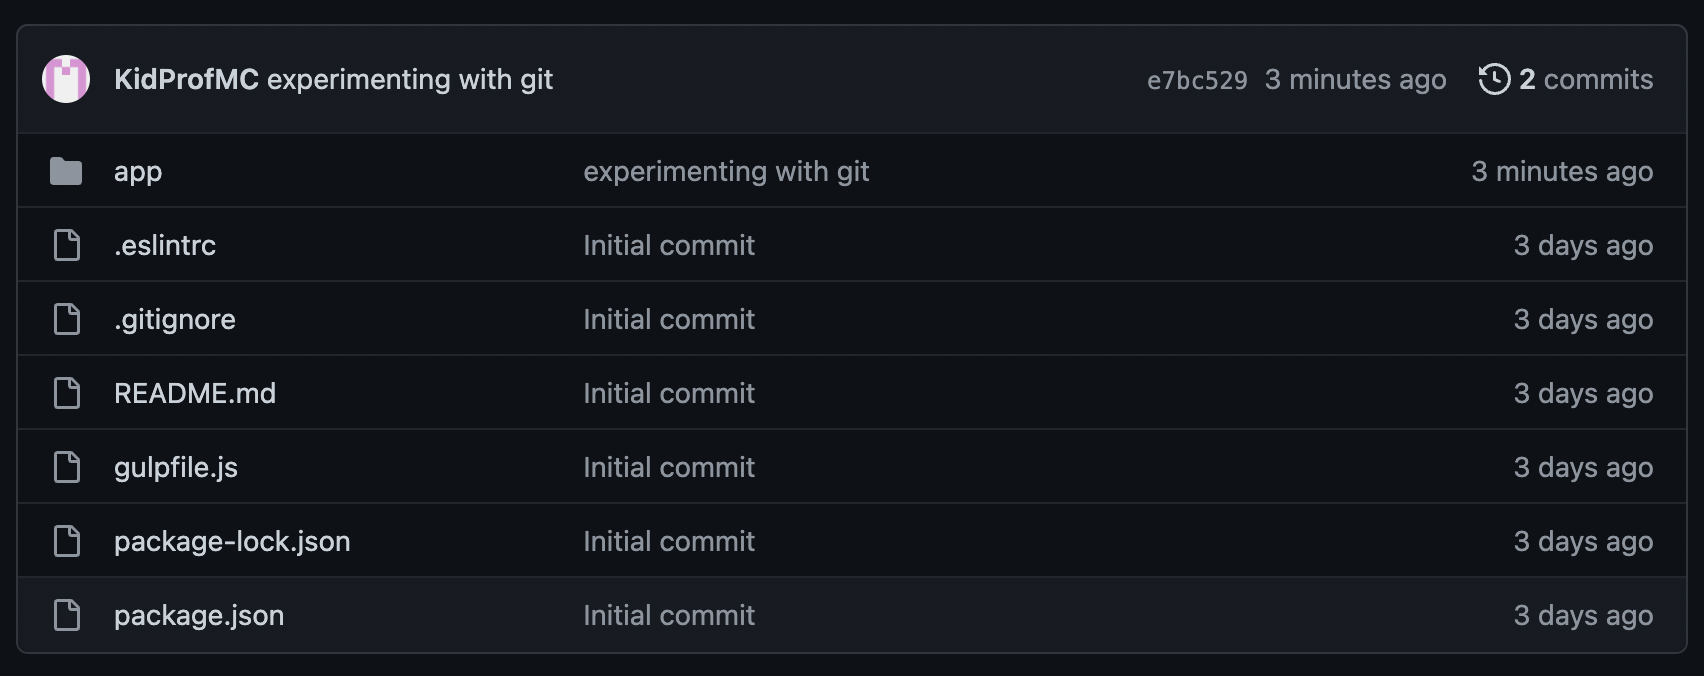
\includegraphics[width=12cm]{images/ch3-firstpushsuccess.png}
\end{center}

There you go, that is the first push. I will not list out the results of \texttt{git status} anymore in future sections, because they are taking too much space, but bear in mind running \texttt{git status} regularly is very useful.

\section{A typical day using Git}
\label{sec:gcmsg}

\textit{Covered in \href{https://www.youtube.com/watch?v=wQmFz-Ggxuo&list=PLjGmdnqrOKuYXiu7lgG5HW71jPEUd1XCm&index=4}{video 3 of the series}}
\vspace{6mm}

It is much more regular after the first push. You just need to remember three steps, add, commit and push.

\begin{lstlisting}[language=bash]
$ git add .
$ git commit -m "your message here"
$ git push
\end{lstlisting}

\texttt{git add} includes the changes you have made to be ready for the commit. 

\texttt{git commit} seals and confirms your changes into one chunk, and adds a commit message. The \textbf{commit message} should be meaningful, summarising what you have achieved with these code changes.

\texttt{git push} uploads the commit from your local machine to GitHub. \textbf{Push} is another fancier word for upload
\vspace{6mm}

You should perform these three steps whenever you have made some progress on your code, as if it is a save button. Practice makes perfect!

\subsection*{When do I have to set name and email like in the previous section?}

Every time you are using a new computer.

\subsection*{When do I have to add \texttt{--set-upstream} when pushing?}

Every time you are pushing a new branch to GitHub. You don't need to remember to do so because Git will reminds you anyways as shown in the previous section.

\section{Visualising}
\label{sec:sublime}
Git is a command line tool and is best used through the command line. Again, you will come across some situations where only command line is available (e.g. when accessing a remote server). 

However, it is acceptable if you just want to visualise the git commit history. Just don't run any commands using them. The following are two software recommended by me to do so. Sublime Merge looks nicer while Git Graph is visible inside VS Code. 

\subsection*{Sublime Merge}

Download Sublime Merge by following \href{https://www.sublimemerge.com/}{this link}.\footnote{Link: \url{https://www.sublimemerge.com/}} It should be straightforward. 

After installing, open the repository folder. The commit history is displayed.

\begin{center}
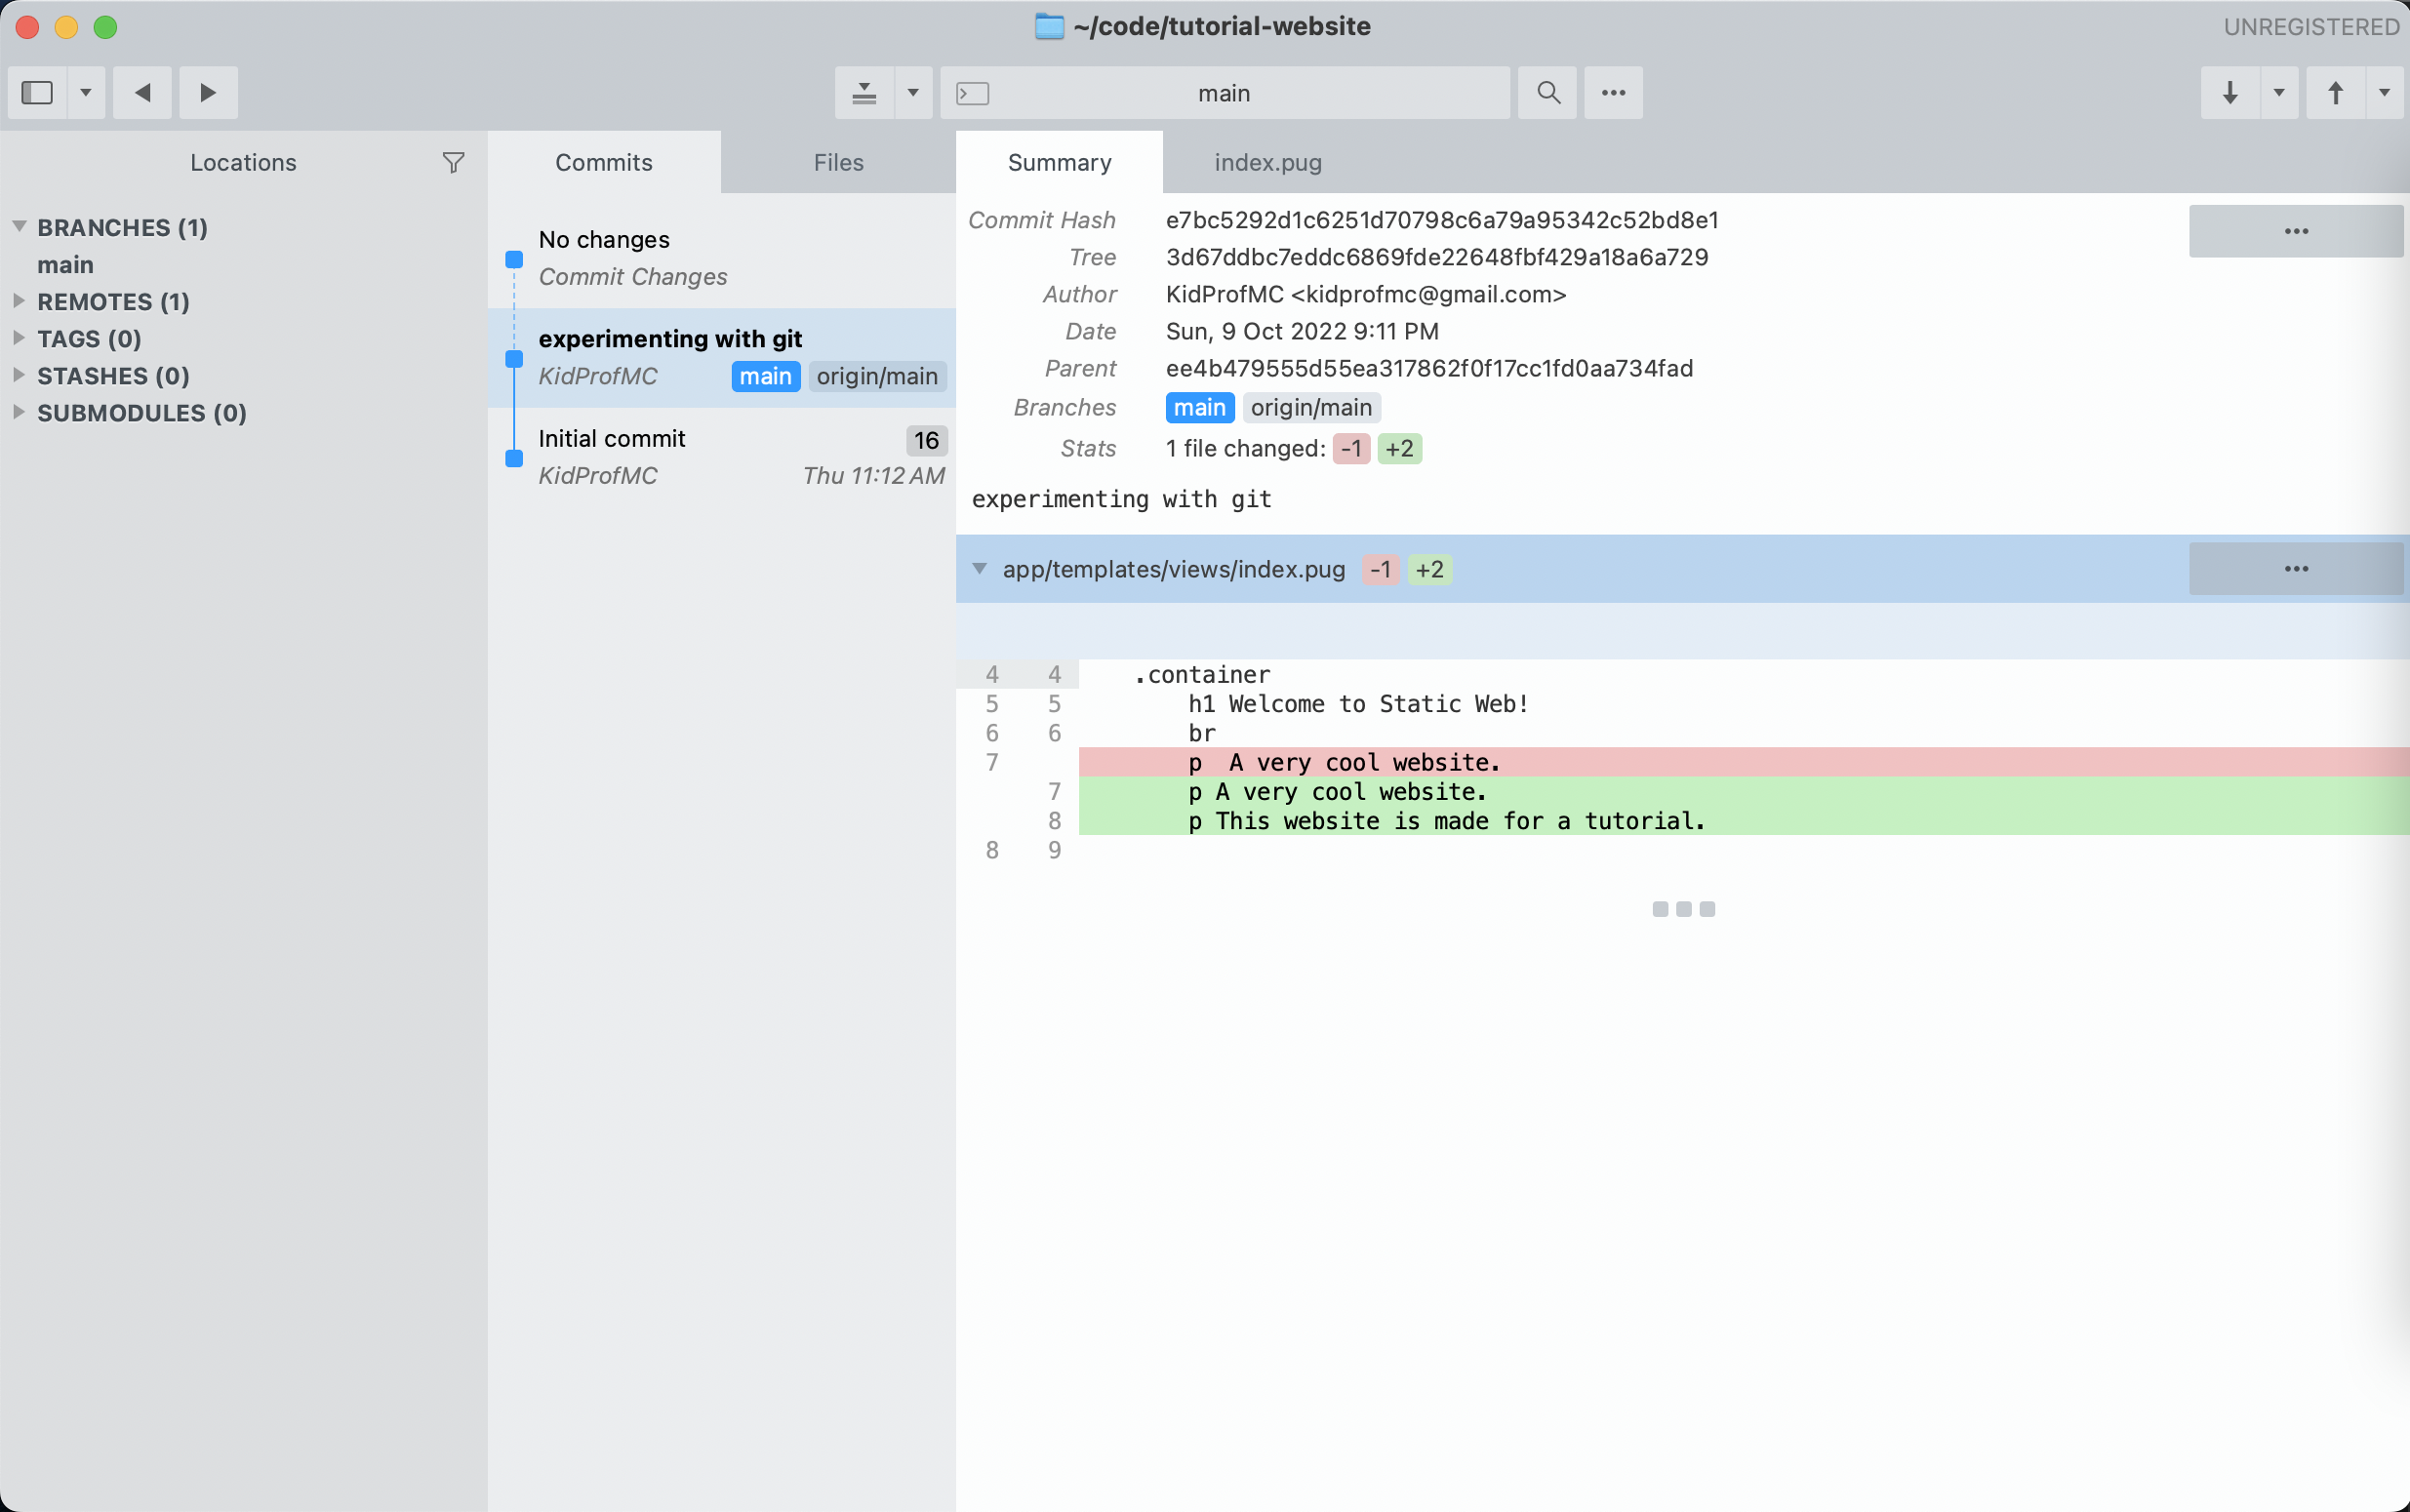
\includegraphics[width=15cm]{images/ch3-sublimemerge.png}
\end{center}

\subsection*{Git Graph}

Git Graph is a VS Code extension, download it inside VS Code.

\begin{center}
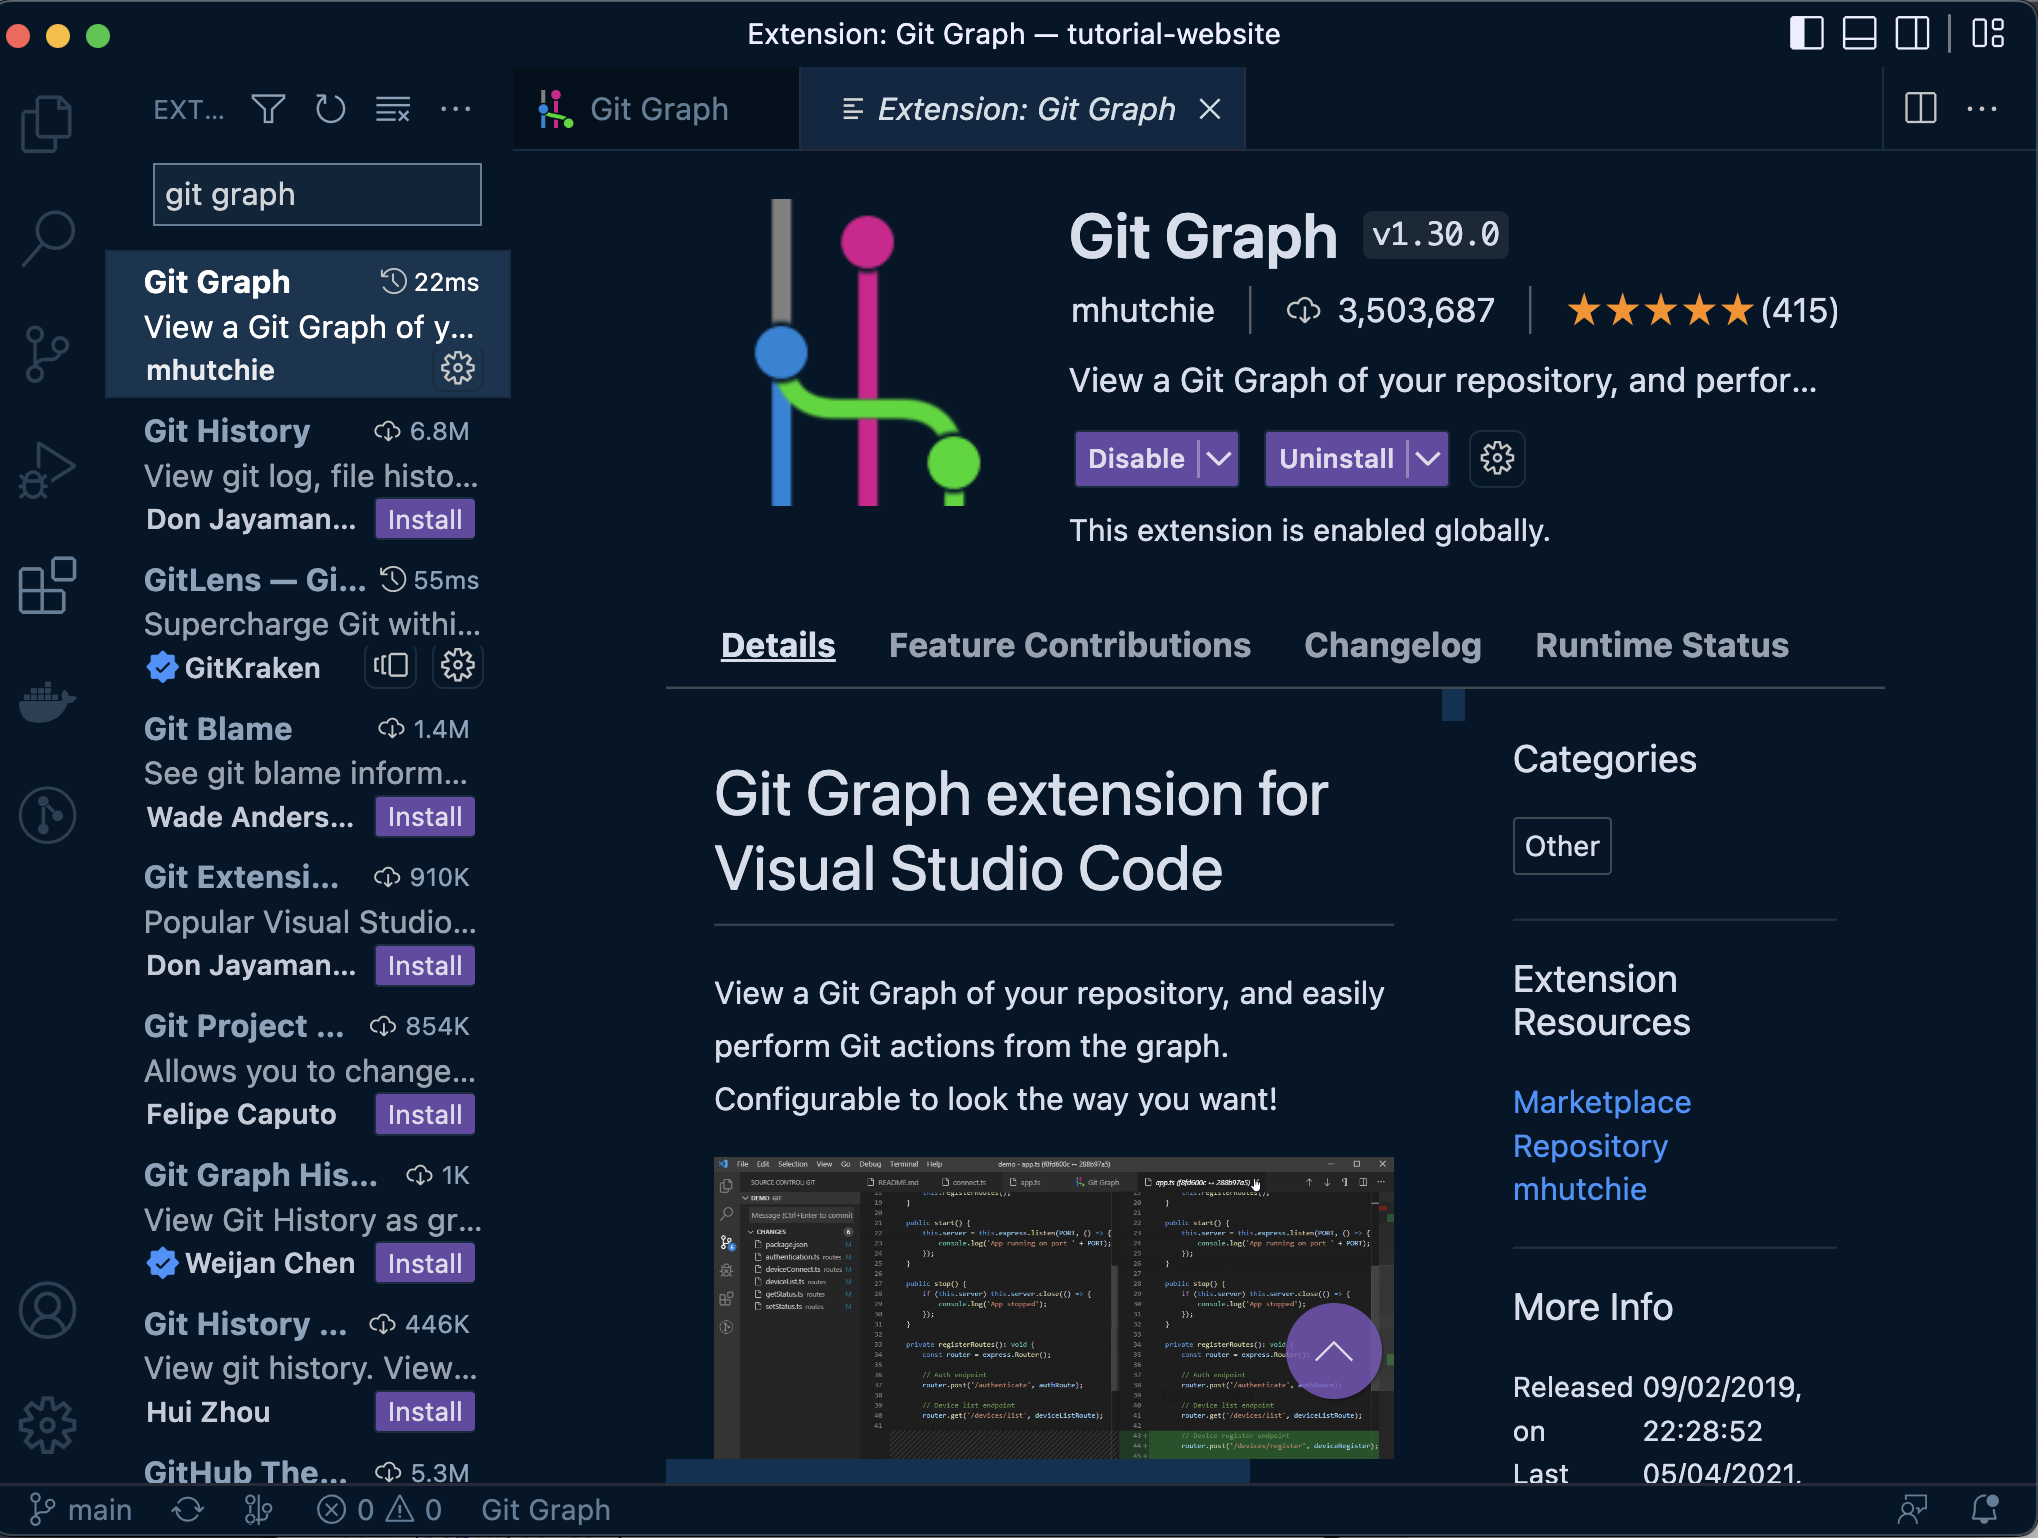
\includegraphics[width=13cm]{images/ch3-gitgraph0.png}
\end{center}

Press \texttt{cmd+shift+P} or \texttt{ctrl+shift+P} to open the VS Code command bar, type \texttt{Git Graph: View Git Graph}

\begin{center}
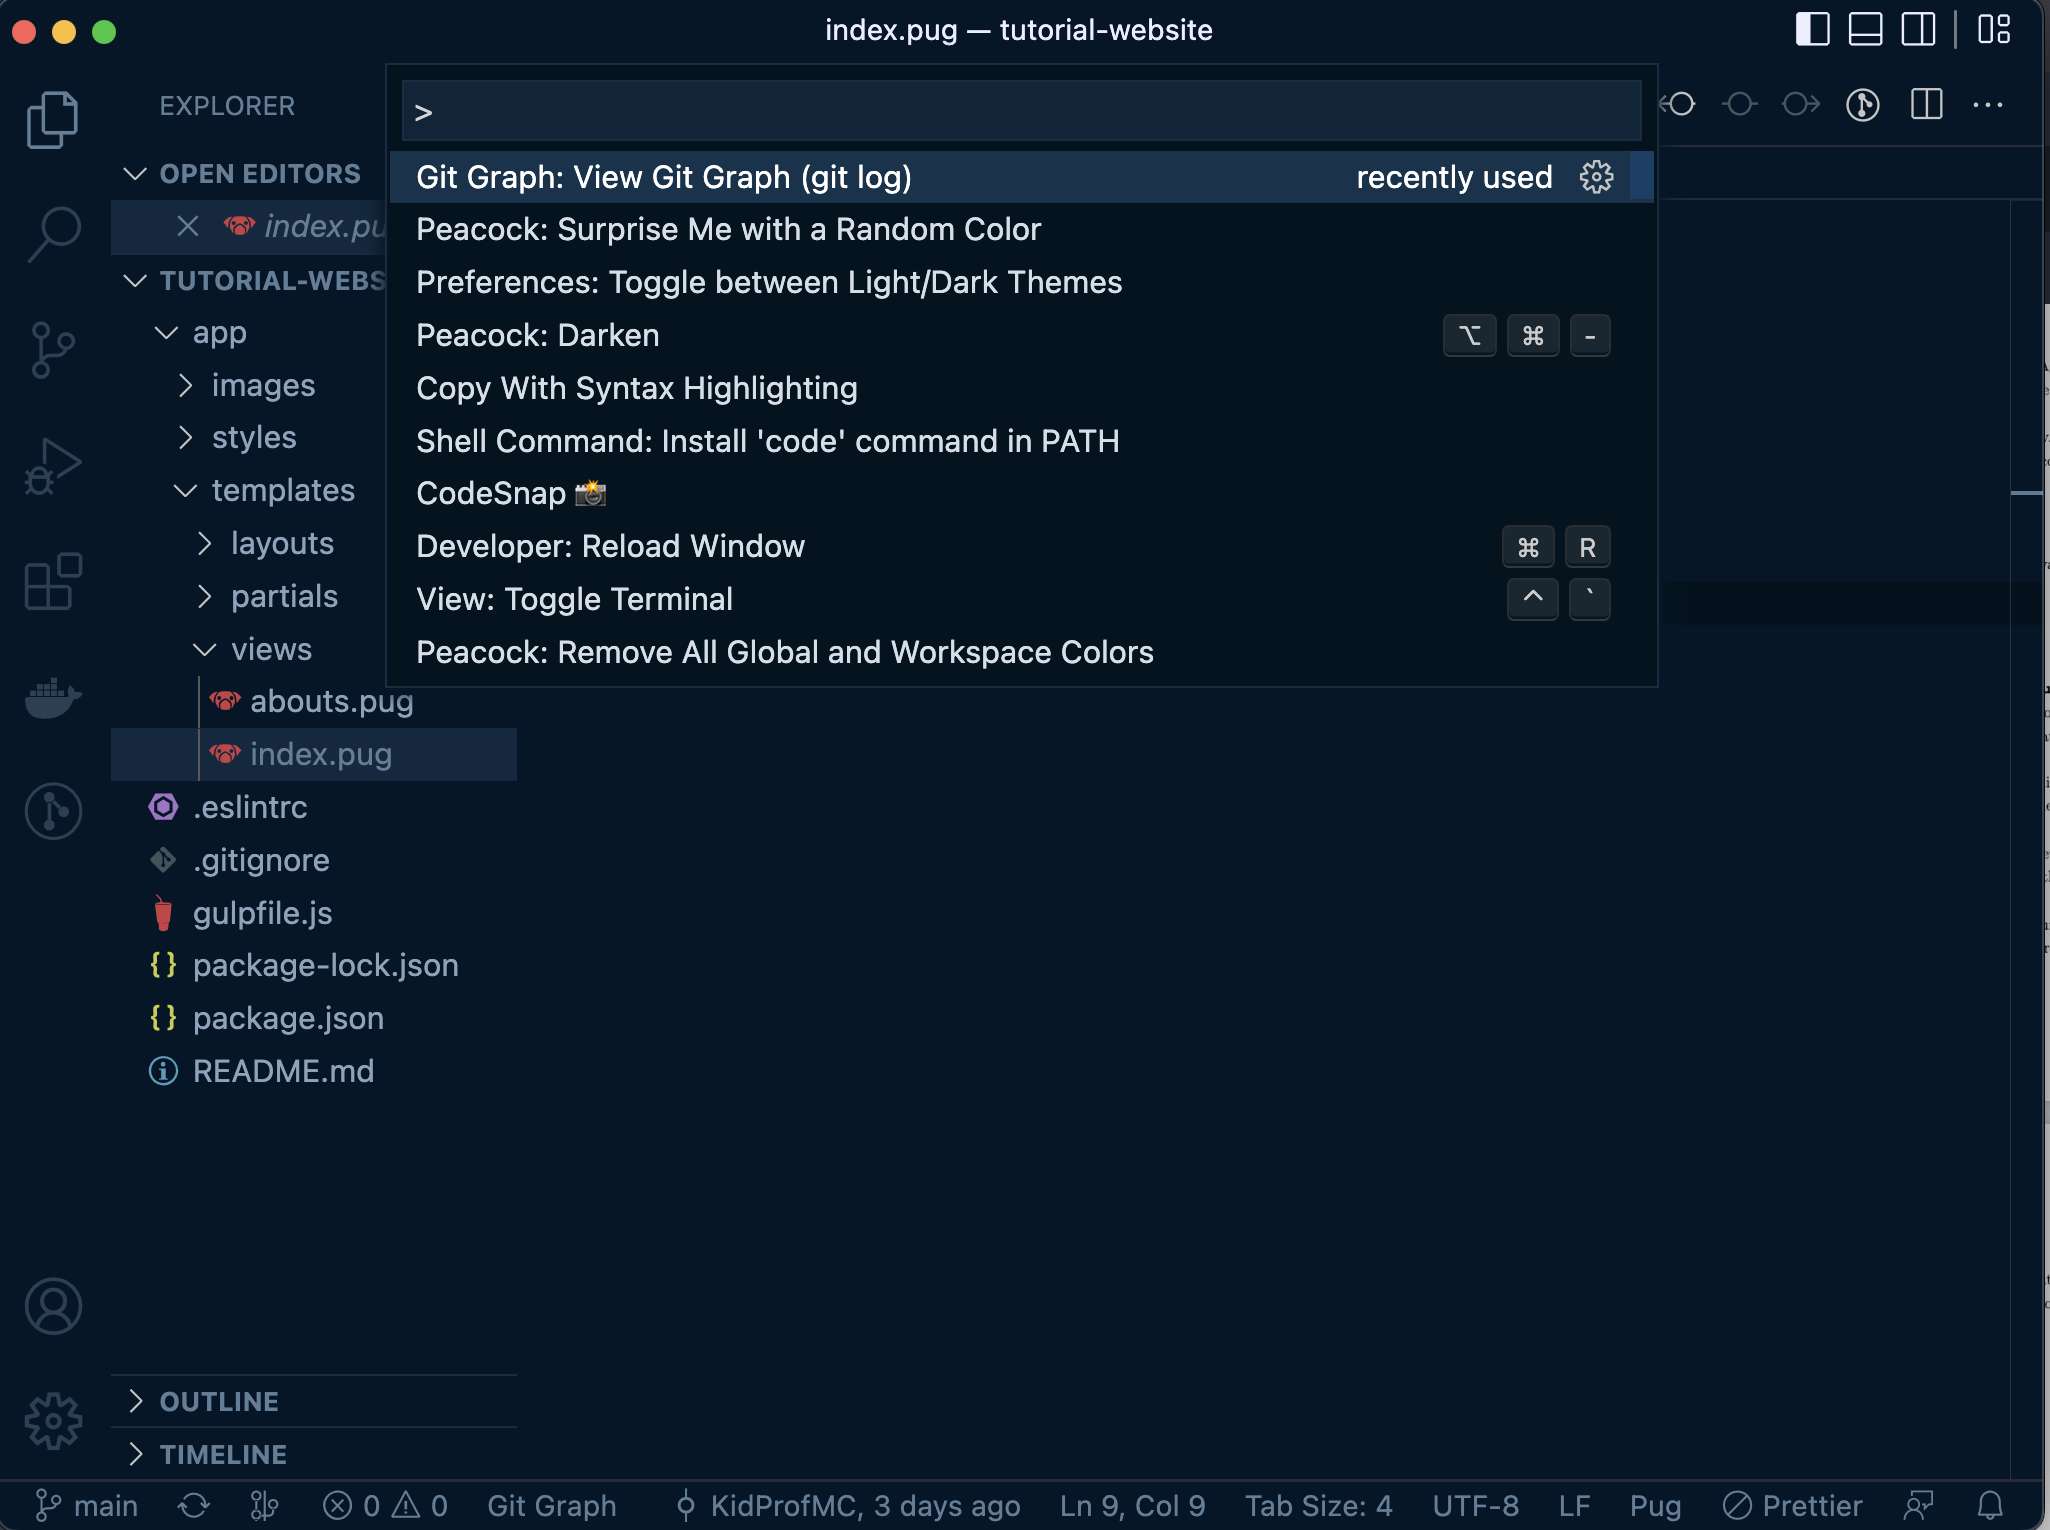
\includegraphics[width=13cm]{images/ch3-gitgraph1.png}
\end{center}

The commit history is displayed.

\begin{center}
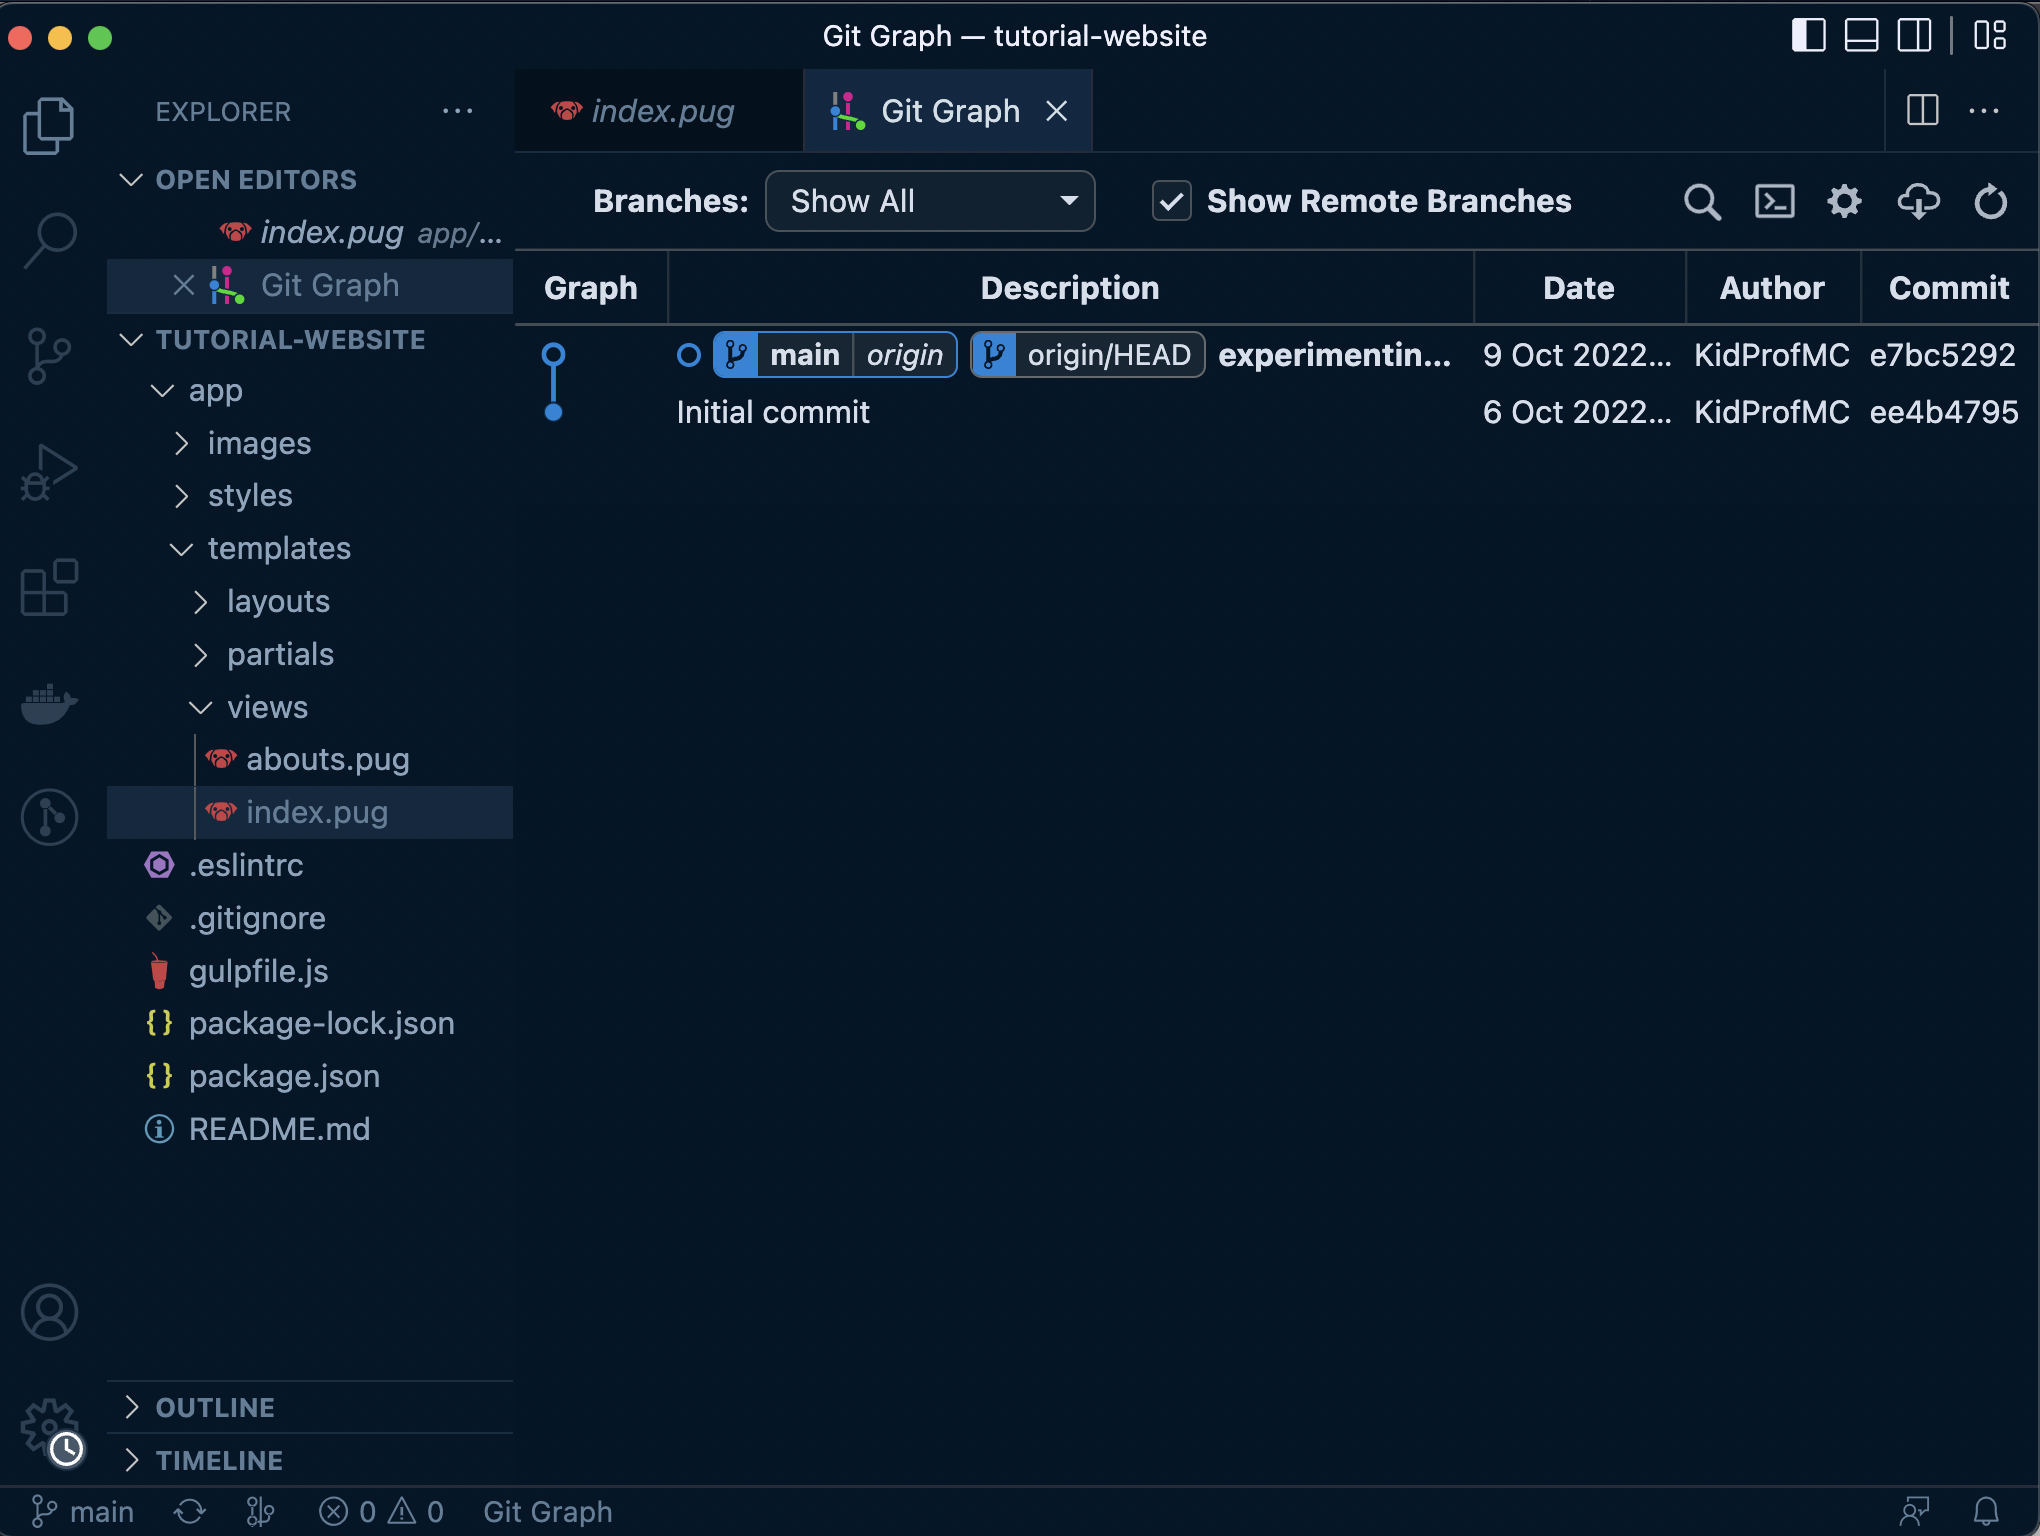
\includegraphics[width=13cm]{images/ch3-gitgraph2.png}
\end{center}

\section{Something went wrong?}
\label{sec:gitpractice}

Anytime if you are unsure about what is happening with Git, \textbf{\texttt{git status}} is your best friend! It will display information about current situation, it might also contains some hints on which command(s) you need to run to get out of nasty situations.
\vspace{6mm}

If you added a files that you don't want to push, and you have not committed, you can try \texttt{git restore <file>} to revert the changes for a particular file, or \texttt{git restore .} to revert all changes.

However, if you made some irreversible/ hard to reverse mistakes, which everybody will at some point in time. For example, you have made a commit at the wrong branch but haven't pushed, or you failed to fix a merge conflict. 

In these cases, let's give up and use a cheesy way to fix it. Move all your code to another location so that you remember what you have changed, clone the repository from GitHub again, then apply your changes to the new copy of the code, but with the mistakes fixed. It is completely fine, and sometimes the easiest way to do something.

Some of you who have learnt Git before may realise that there are other ways of using Git, mine is a more traditional command line approach, if you want to know why you can refer to \cref{sec:githubdesktop}.

\section{Repositories}

\textit{Advanced}
\vspace{6mm}

Again, repository is a fancier name for project. Now we will look closely at this concept, and explain how to establish the relationship between your local code and the GitHub code.

\subsection{Creating a repository on GitHub}
\label{sec:gituploadgithub}

\textit{\textbf{WARNING: } You can only do so when the repository is empty. If the GitHub repository is not empty, you will need to create a new one.}

It is as simple as pressing a "New" button on the GitHub website, then fill in some simple details, such as your repository name and whether you would like your repository to be publicly visible or private, the decision is yours.

You can add a \hyperref[sec:readme]{\texttt{README.md}} or \hyperref[sec:gitignore]{\texttt{.gitignore}}, the usage of such files will be explained in the \hyperref[sec:projstructure]{next chapter}. However, it would make the repository no longer empty and you will have trouble \hyperref[sec:gituploadgithub]{uploading local code to the new repository.}

\subsection{Uploading existing local code to a new GitHub repository}
\label{sec:gitinit} 

Use \texttt{git init} in the folder with all your projects.

The use of \texttt{git branch -M main} is to change the name of the default branch from "master" to "main". A decision that GitHub made in 2020.\footnote{More info: \url{https://www.jumpingrivers.com/blog/git-moving-master-to-main/}}

Then follow your normal routine of adding and committing as above in \cref{sec:gcmsg}. There is a convention naming the first commit "init" or "initial commit".

Then \texttt{git remote add origin} is to establish the linkage between the local code and the GitHub repository, so that Git knows where to push to when you run \texttt{git push}, except for the first time, you need to run \texttt{git push -u origin main}.

\begin{lstlisting}[language=bash]
# KidProf in ~/code/your-project
$ git init

# No need to remember, copy from the GitHub docs
$ git branch -M main 

$ git add .
$ git commit -m "init"

# No need to remember, copy from the GitHub docs
$ git remote add origin git@github.com:KidProfMC/git-practice.git
$ git push -u origin main
\end{lstlisting}

\begin{figure}[h]
\centering
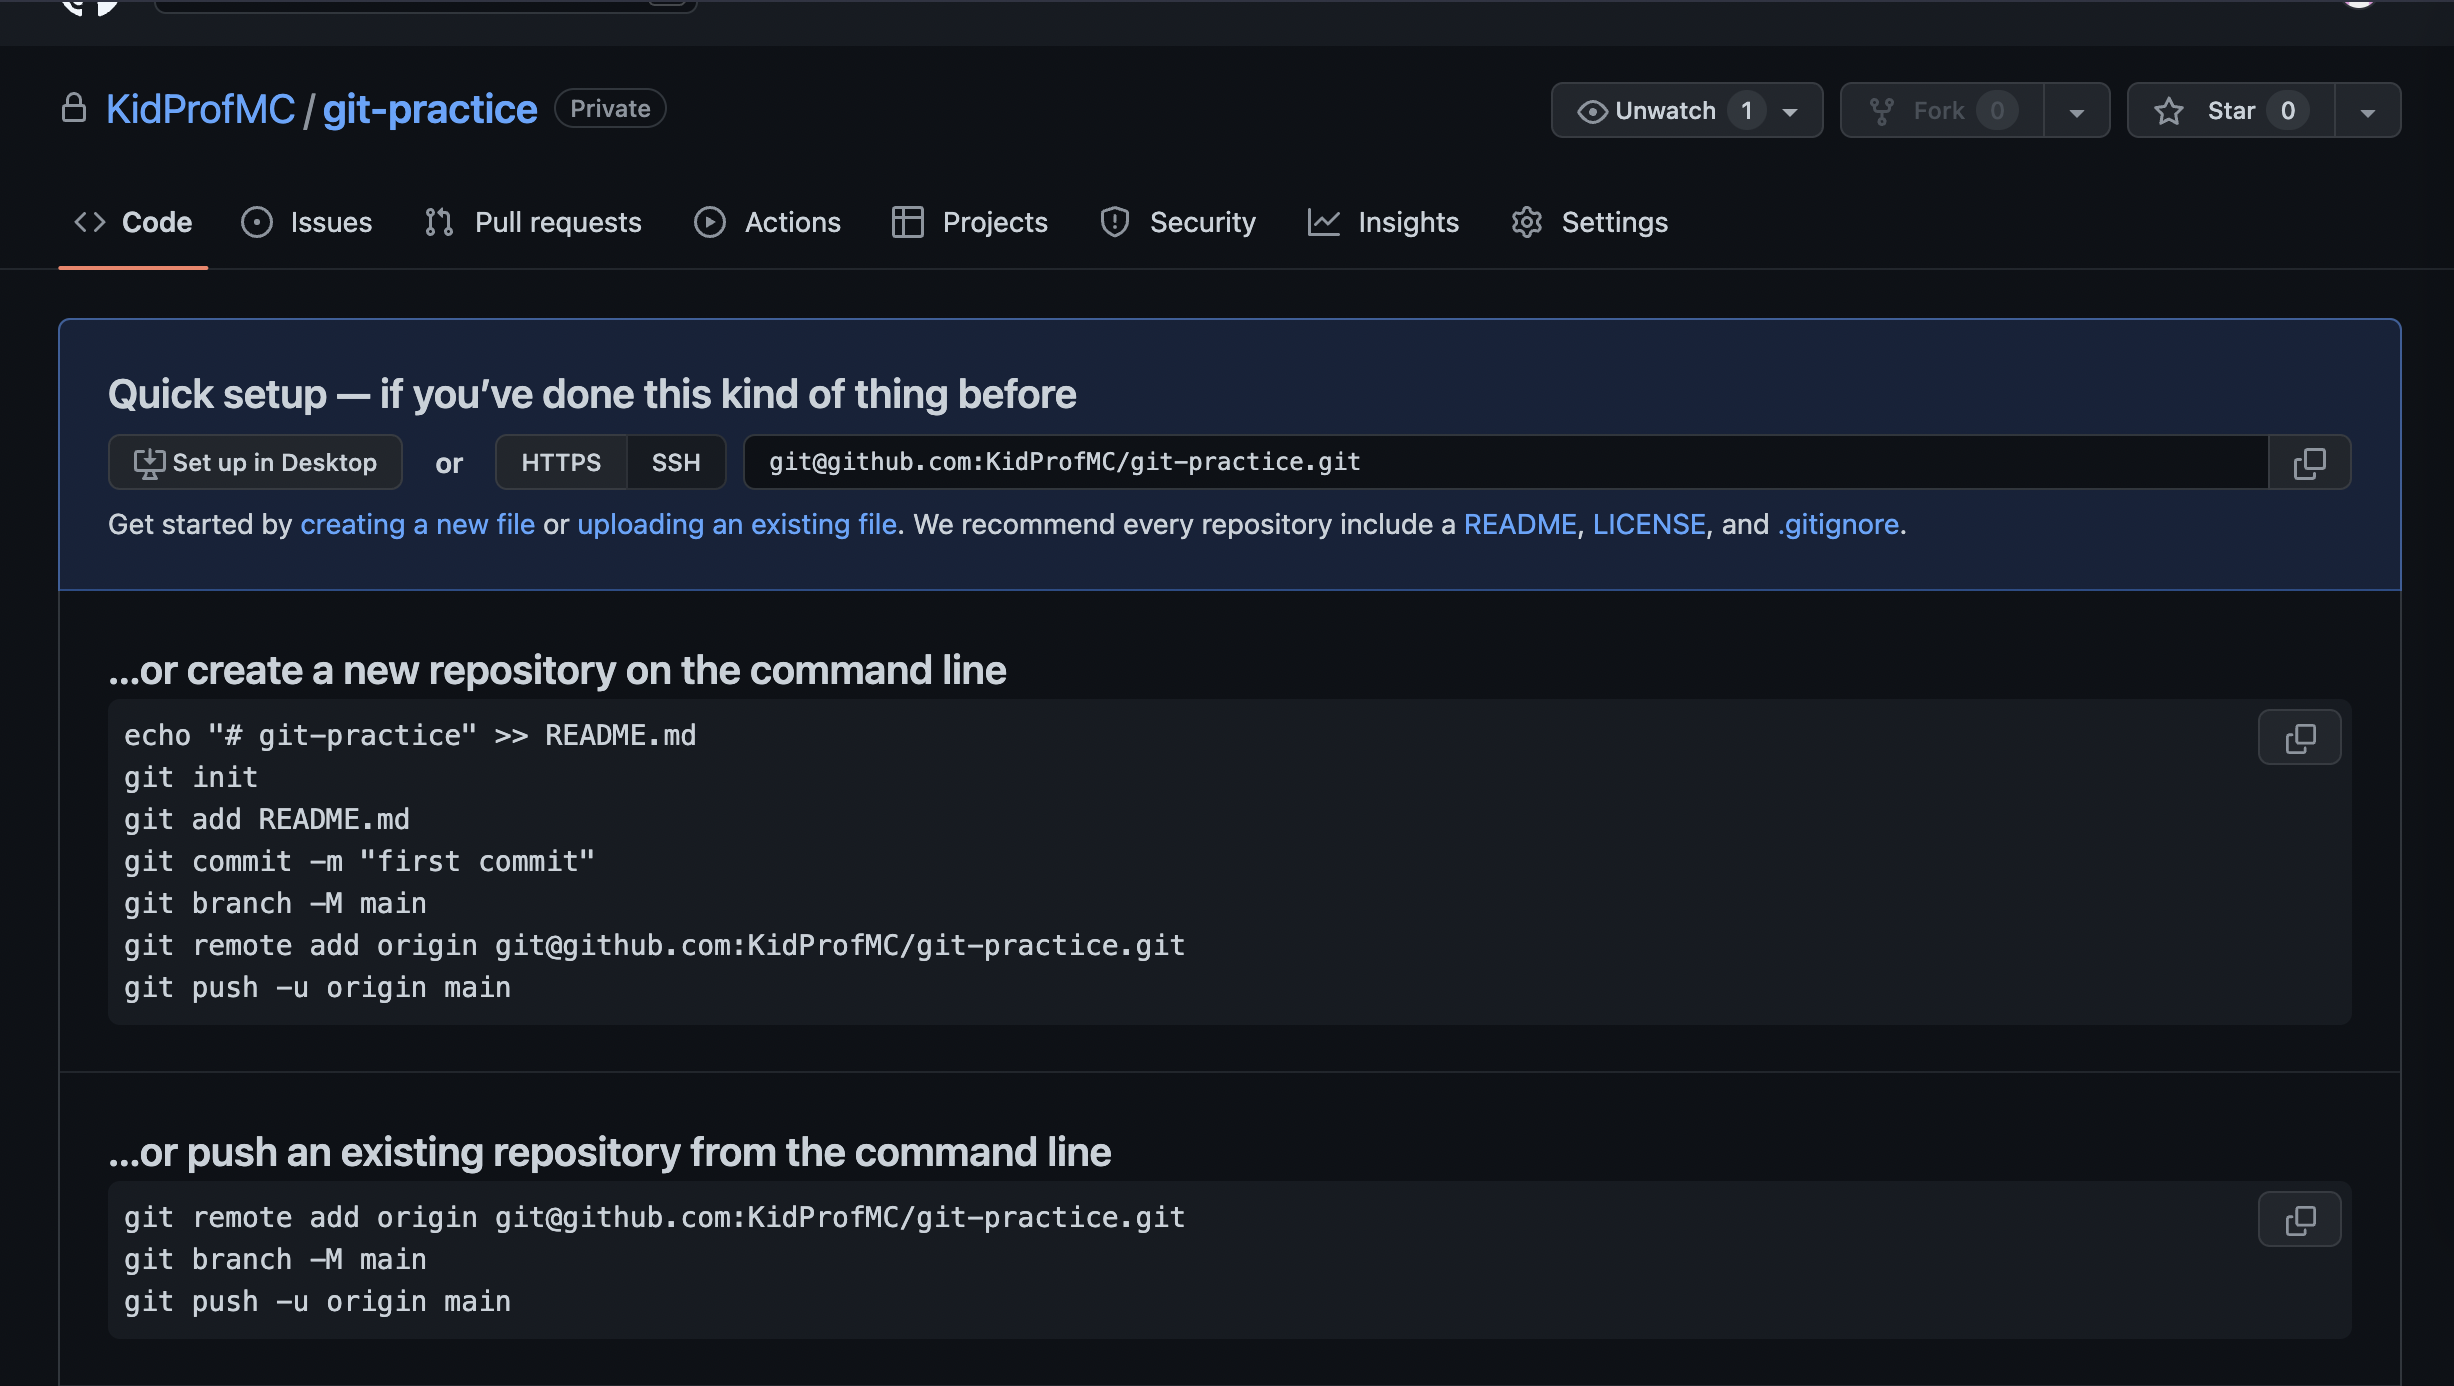
\includegraphics[width=15cm]{images/ch3-newrepocode.png}
\caption{The documentation on GitHub serves you well}
\end{figure}

\subsection{Downloading code from GitHub to local device}
\label{sec:gitclone}

Use \texttt{git clone} followed by the URL provided by GitHub, then a new folder with the repository name would be created with all the code inside. This is the method that we used in \cref{sec:install7}.

\begin{lstlisting}[language=bash]
# KidProf in ~/code
$ git clone git@github.com:KidProfMC/git-practice.git
$ cd git-practice
\end{lstlisting}

\subsection{\texttt{.git} folder}

The \texttt{.git} folder contains everything that git needs to know to function normally, the commit history, the GitHub repository that it is linked to, etc.. If you remove the \texttt{.git} folder from your local device through the file explorer or finder (you need to enable the setting "show hidden files and folders"), or by the command \texttt{rm -rf .git}, all git information would be deleted.


\chapter{Project Structure}
\label{sec:projstructure}
% Old Ch. 4

\textit{Covered in \href{https://www.youtube.com/watch?v=fbbjnhs4nyo&list=PLjGmdnqrOKuYXiu7lgG5HW71jPEUd1XCm&index=3}{video 2 of the series}}
\vspace{6mm}

We will tour around the project and explain how my template works. It is just a brief overview, you do not need to remember and understand every detail, the most important thing to learn is how to use them, which are be taught in \cref{sec:pug1} and also the chapters to come.

\section{Overview}

The \texttt{app} folder contains everything you need to generate the website. The Pug files, the styles written in Less, JavaScript files, images, etc.. Then by running \texttt{npm run build}, commanding the \texttt{gulpfile.js} and \texttt{node\textunderscore modules} to work together, it translates the Pug files into HTML files, less styles into CSS files, and copies other files to the \texttt{docs} folder. The \texttt{docs} folder is the final output of the website, we can open the HTML files directly using a browser.

\section{Pug files}

Pug files act as template files. They are translated into HTML files and provide the basic structure of the web page. All Pug files should be put inside \texttt{app/templates}.

\subsection*{Views}

The \texttt{app/templates/views} folder contains the content body of each page. Each Pug file in this folder would be translated to an HTML file with the same name in \texttt{docs}. As you can see, \texttt{abouts.pug} is translated into \texttt{abouts.html} while \texttt{index.pug} is translated into \texttt{index.html}. They all \texttt{extends ../layouts/default}, meaning that they follow the layout in \texttt{app/templates/layouts/default.pug}, which we will look at in a second. (Reminder: \texttt{..} means previous directory)

\texttt{index.pug} (later translated to \texttt{index.html}) is the homepage of the web site. When you host the web page onto a web server, the index page will be shown when you just type in the URL without specifying which HTML file you want to read. You are advised to have an \texttt{index.pug} file in every project.

\subsection*{Layouts}

The \texttt{app/templates/layouts} folder contains \texttt{default.pug}. It is a template for \textbf{all} pages. It includes common elements like the page title, the styles import, the navbar and the footer. (also checkout \cref{fig:puglayouts})

Then under \texttt{block content} in line 55, each page in the \texttt{views} folder inserts their own content under this block. Knowing the exact syntax is not required.

\begin{lstlisting}[language=pug]
//- app/templates/layouts/default.pug
doctype html
html
	head
		...
		link(href="styles/site.css", rel="stylesheet")
		...
	body
		#header
			include ../partials/navbar.pug
		#body
			block content
		.container: #footer
			include ../partials/footer.pug
        ...
\end{lstlisting}

\subsection*{Partials}

The navbar and footer are separated from the \texttt{default.pug} to make it cleaner. They are put in the \texttt{app/templates/partials} folder, and got included in \texttt{default.pug} in lines 38 and 61 respectively.

\begin{figure}[h]
\centering
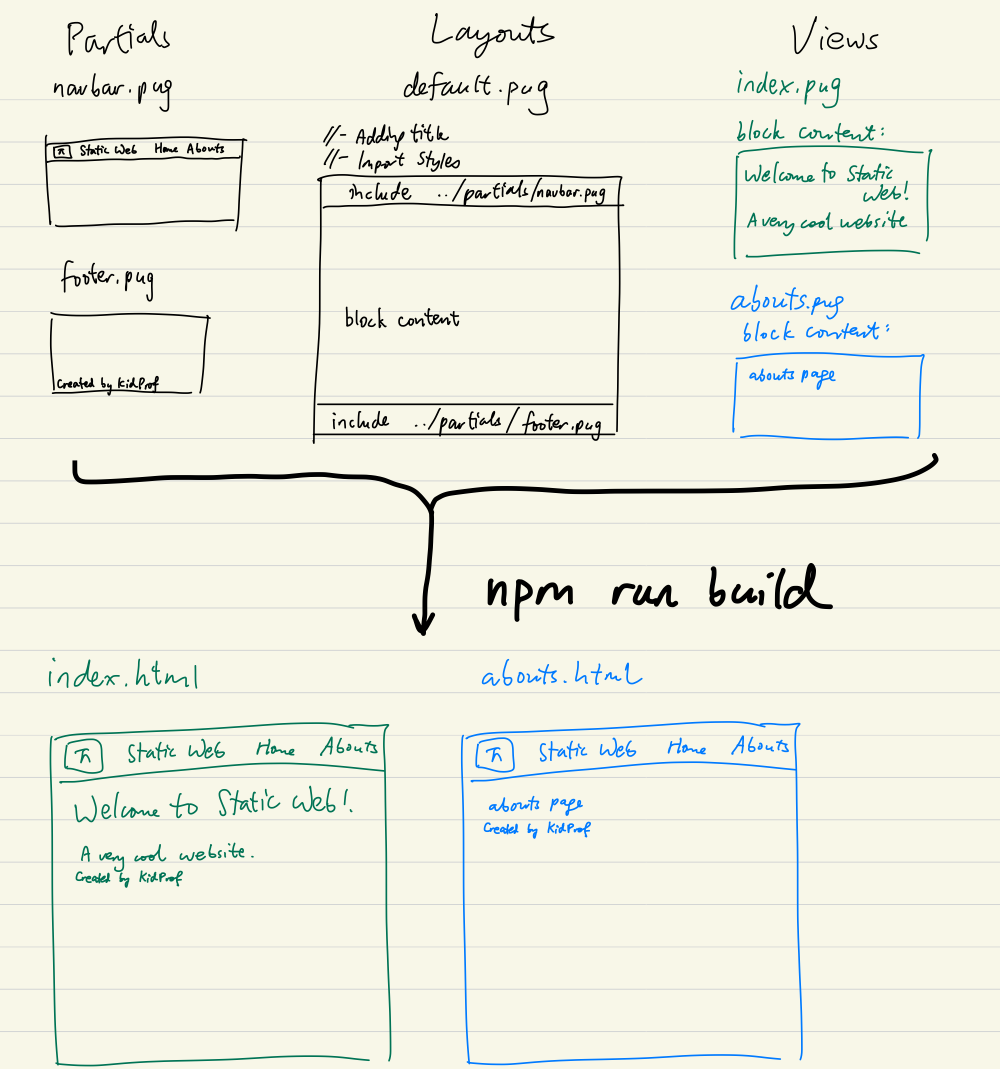
\includegraphics[width=15cm]{images/ch4-puglayouts.png}
\caption{Overview on how Pug files are translated}
\label{fig:puglayouts}
\end{figure}

\section{Styling files}
\label{sec:lesslayout}

We will be using less files for styling in place for CSS, which are placed under \texttt{app/styles}. We will call them \textbf{styling files} in this piece of notes. The \texttt{site.less} file includes all files under the \texttt{app/styles/site} folder, \textbf{remember to add the file to \texttt{site.less} whenever you are creating a new less file}. 

The files under the \texttt{site} folder should be where you write the styles. By convention, \texttt{layout.less} should contain styles that is used in all/ multiple pages; \texttt{variables.less} should contain all variables; and other files should contain styles that is only used in the page with the same name as the style file. This is just a convention, there is nothing to enforce it until \cref{sec:confinestyles}.

When we run \texttt{npm run build}, the styles got translated into CSS and put into a single file \texttt{docs/styles/site.css}. The stylesheet is imported into all HTML files in line 18 of \texttt{layout.pug}.

\section{Images and other assets}

Place all the images or other assets you need for the website under \texttt{\textbf{app}/images} folder. For JavaScript files, you may create a new \texttt{app/js} folder to store them. Do not put them inside \texttt{docs}! As changes you made in the \texttt{docs} folder will be overwritten when you run \texttt{npm run build} again.

\section{Website generation}
\label{sec:webgen}
We kept mentioning \texttt{npm run build} as if it is some sort of magic, now it's time to look a little bit closer. These files are not our focus and \textit{you do not need to edit these files at all throughout the notes.}

\subsection{\texttt{package.json}}

This file contains basic information about our project (change the name and description if you like). What is more important is the dependencies and the devDependencies, it tells \texttt{npm}\footnote{stands for Node Package Manager} which libraries we need to run this project, it is written by me, so all you have to do is to run \texttt{npm install} (what you did already in chapter 1), and it knows what to install for you, without the need of you specifying what to install.

Also the scripts section specifies what will be run on \texttt{npm run ...}, from the line \texttt{"build": "gulp build"}, it means the command \texttt{gulp build} will be run when we run \texttt{npm run build}. More in \cref{sec:gulpfile}.

\begin{lstlisting}[language=]
{
  "name": "static-web-sandbox",
  "version": "2.0.0",
  "description": "A very cool website.",
  "dependencies": {
    "gulp": "^4.0.0"
  },
  "devDependencies": {
    "@babel/core": "^7.2.0",
    "@babel/preset-env": "^7.2.0",
    "gulp-babel": "^8.0.0",
    "gulp-changed": "^3.2.0",
    "gulp-eslint": "^5.0.0",
    "gulp-imagemin": "^5.0.3",
    "gulp-less": "^4.0.1",
    "gulp-pug": "^4.0.1",
    "less-plugin-autoprefix": "^2.0.0"
  },
  "scripts": {
    "test": "echo \"Error: no test specified\" && exit 1",
    "build": "gulp build"
  },
  "license": "ISC"
}
\end{lstlisting}

\subsection{\texttt{node\textunderscore modules} folder}

This folder is automatically generated when you run \texttt{npm install}\footnote{To verify, remove this folder using \texttt{rm -rf node\textunderscore modules} and run \texttt{npm install} again.} It contains the library files you need to run this project, the project would not run without this folder. 

\subsection{\texttt{package-lock.json}}

This is an automatically generated file, it outlines in detail which version of the dependencies are installed. It automatically updates when you run \texttt{npm install}.

\subsection{\texttt{gulpfile.js}}
\label{sec:gulpfile}

This file is responsible for the translation process. As you can see, the task \texttt{pug} translates each \texttt{.pug} file under \texttt{app/templates/views} to HTML files and put them under \texttt{docs}. Similar translation happens for less files. The JavaScript files, images and fonts are copied to the \texttt{docs} folder.

Finally, the task \texttt{build} runs all the above commands. Therefore, \texttt{gulp build} does what is is supposed to do. 

\begin{lstlisting}[language=JavaScript]
// gulpfile.js
...

//pug to html conversion
gulp.task('pug', function(){
  return gulp.src("app/templates/views/*.pug")
  .pipe(changed("docs/")) //pipe files only if changed 
  .pipe(pug({pretty:true})) //pug to html
  .pipe(gulp.dest('docs/'));
});

//less to css conversion
gulp.task('styling', function(){
  return gulp.src("app/styles/site.less")
  .pipe(changed("docs/styles")) //pipe files only if changed 
  .pipe(less({
    plugins: [autoprefix]
  })) //less to css
  .pipe(gulp.dest('docs/styles'));
});

gulp.task('js',function(){ ... });
gulp.task('imagecopy',function(){ ... });
gulp.task('fontcopy',function(){ ... });

gulp.task('build',gulp.series('js','pug','styling','imagecopy','fontcopy'));

\end{lstlisting}

\subsection{\texttt{docs} folder}
\label{sec:docs}

This folder is automatically generated when you run \texttt{npm run build}.\footnote{To verify, remove this folder using \texttt{rm -rf docs} and run \texttt{npm run build} again.} It is the output folder of the whole project, you can directly open the HTML files inside the folder. You should upload this folder to web servers in order to host it.

We can reference the images and JavaScript files using \texttt{images/$<$filename$>$} and \texttt{js/$<$filename$>$} because they are copied to \texttt{docs/images} and \texttt{docs/js} respectively, we reference them in the perspective of the resultant HTML files which are put under \texttt{docs}.
\vspace{6mm}

\textbf{IMPORTANT: Do NOT edit anything in the \texttt{docs} folder. Changes will be overwritten when you run \texttt{npm run build} again.}

\subsection{\texttt{.gitignore}}
\label{sec:gitignore}

Because the \texttt{node\textunderscore modules} folder and the \texttt{docs} folder can be automatically generated on your own local machine. There is no need to put these onto GitHub. The \texttt{.gitignore} file lets you state the files and folders that you do not want to push to GitHub. It includes the two folders I have mentioned, and some others that are out of our scope.

\begin{figure}[h]
\centering
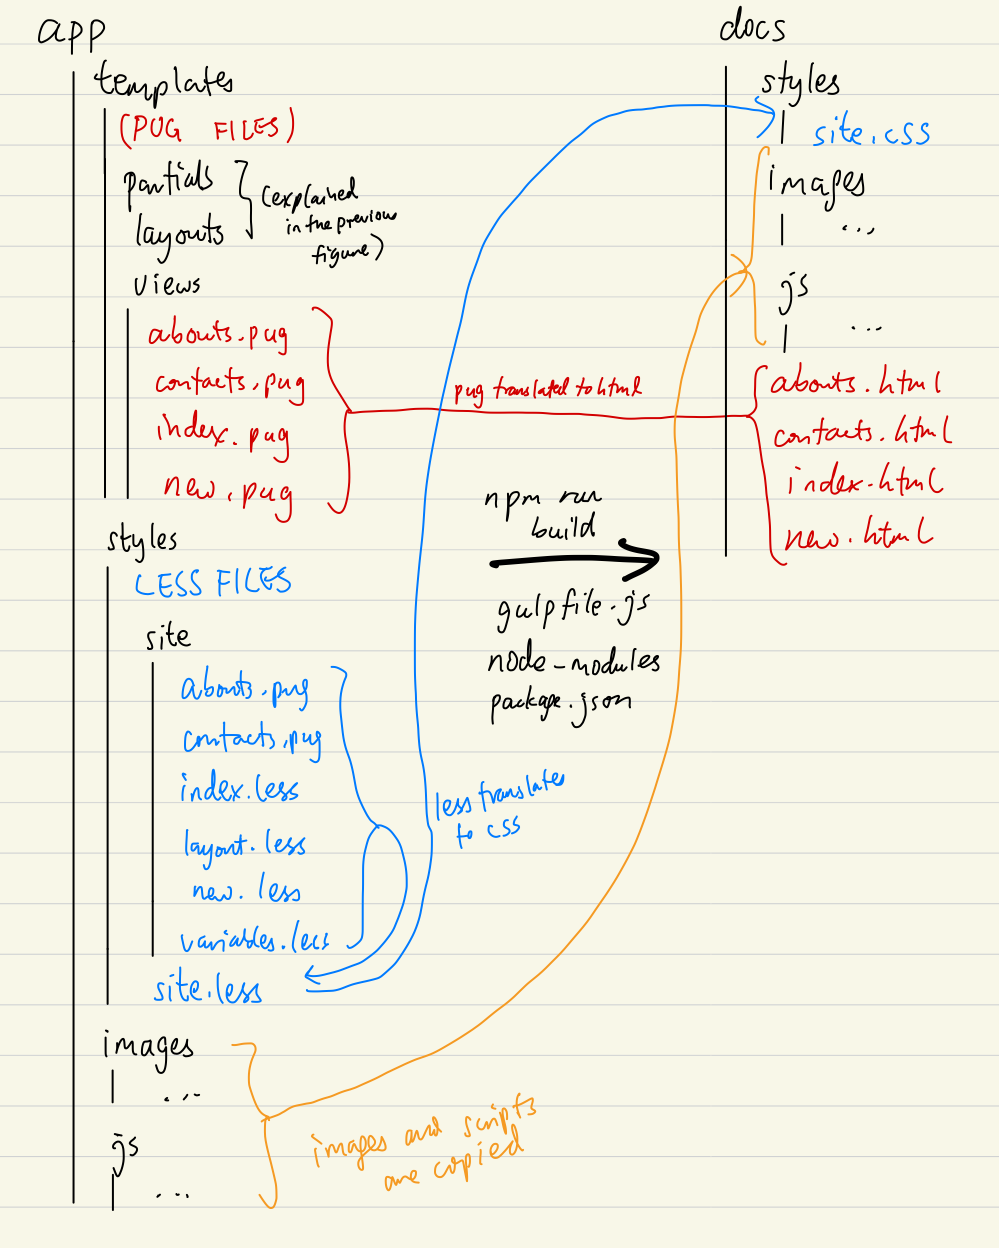
\includegraphics[width=15cm]{images/chn5-full-translation.png}
\caption{Overview of the translation process}
\end{figure}

\section{Other files}

\subsection{\texttt{README.md}}
\label{sec:readme}

This file serves as a documentation. It will be displayed on GitHub. You should write a description of your project, and how to install and use it in this file. The syntax is a bit weird, refer \href{https://docs.github.com/en/get-started/writing-on-github/getting-started-with-writing-and-formatting-on-github/basic-writing-and-formatting-syntax}{to this documentation}\footnote{Link: \url{https://docs.github.com/en/get-started/writing-on-github/getting-started-with-writing-and-formatting-on-github/basic-writing-and-formatting-syntax}} if you want to write your own README.

\subsection{\texttt{.eslintrc}}

\textit{Of less importance}
\vspace{6mm}

This file stores the JavaScript settings and the JavaScript version we are using, so as to check for syntax errors when copying JavaScript files from \texttt{app} to \texttt{docs}. \textit{You do not need to edit this file at all.}

\chapter{Project Structure}
\label{sec:projstructure}
% Old Ch. 4

\textit{Covered in \href{https://www.youtube.com/watch?v=fbbjnhs4nyo&list=PLjGmdnqrOKuYXiu7lgG5HW71jPEUd1XCm&index=3}{video 2 of the series}}
\vspace{6mm}

We will tour around the project and explain a little bit on how the website works. It is just a brief overview, you do not need to remember and understand every detail, the most important thing to learn is how to use them, which will be taught in later chapters.

\section{Overview}

The \texttt{app} folder contains everything you need to generate the website. The Pug files, the styles written in Less, JavaScript files, images, etc.. Then by running \texttt{npm run build}, commanding the \texttt{gulpfile.js} and \texttt{node\textunderscore modules} to work together, it translates the Pug files into HTML files, less styles into CSS files, and copies other files to the \texttt{docs} folder. The \texttt{docs} folder is the final output of the website, we can open the HTML files directly using a browser.

\section{Pug files}

Pug files act as template files, we will just call them \textbf{pug files} in this piece of notes. They are translated into HTML files and provide the basic structure of the web page. All Pug files should be put inside \texttt{app/templates}.

\subsection*{Views}

The \texttt{app/templates/views} folder contains the content body of each page. Each Pug file in this folder would be translated to an HTML file with the same name in \texttt{docs}. As you can see, \texttt{abouts.pug} is translated into \texttt{abouts.html} while \texttt{index.pug} is translated into \texttt{index.html}. They all \texttt{extends ../layouts/default}, meaning that they follow the layout in \texttt{app/templates/layouts/default.pug}, which we will look at in a second. (Reminder: \texttt{..} means previous directory)

\texttt{index.pug} (later translated to \texttt{index.html}) is the homepage of the web site. When you host the web page onto a web server, the index page will also be shown when you just type in the URL without specifying which HTML file you want to read. You are advised to have an \texttt{index.pug} file in every project.

\subsection*{Layouts}

The \texttt{app/templates/layouts} folder contains \texttt{default.pug}. It is a template for \textbf{all} pages. It includes common elements like the page title, the styles import, the navbar and the footer. 

Then under \texttt{block content} in line 55, each page in the \texttt{views} folder inserts their own content under this block. Knowing the exact syntax is not required.

\subsection*{Partials}

The navbar and footer are separated from the \texttt{default.pug} to make it cleaner. They are put in the \texttt{app/templates/partials} folder, and got included in \texttt{default.pug} in lines 38 and 61 respectively.

\begin{figure}[h]
\centering
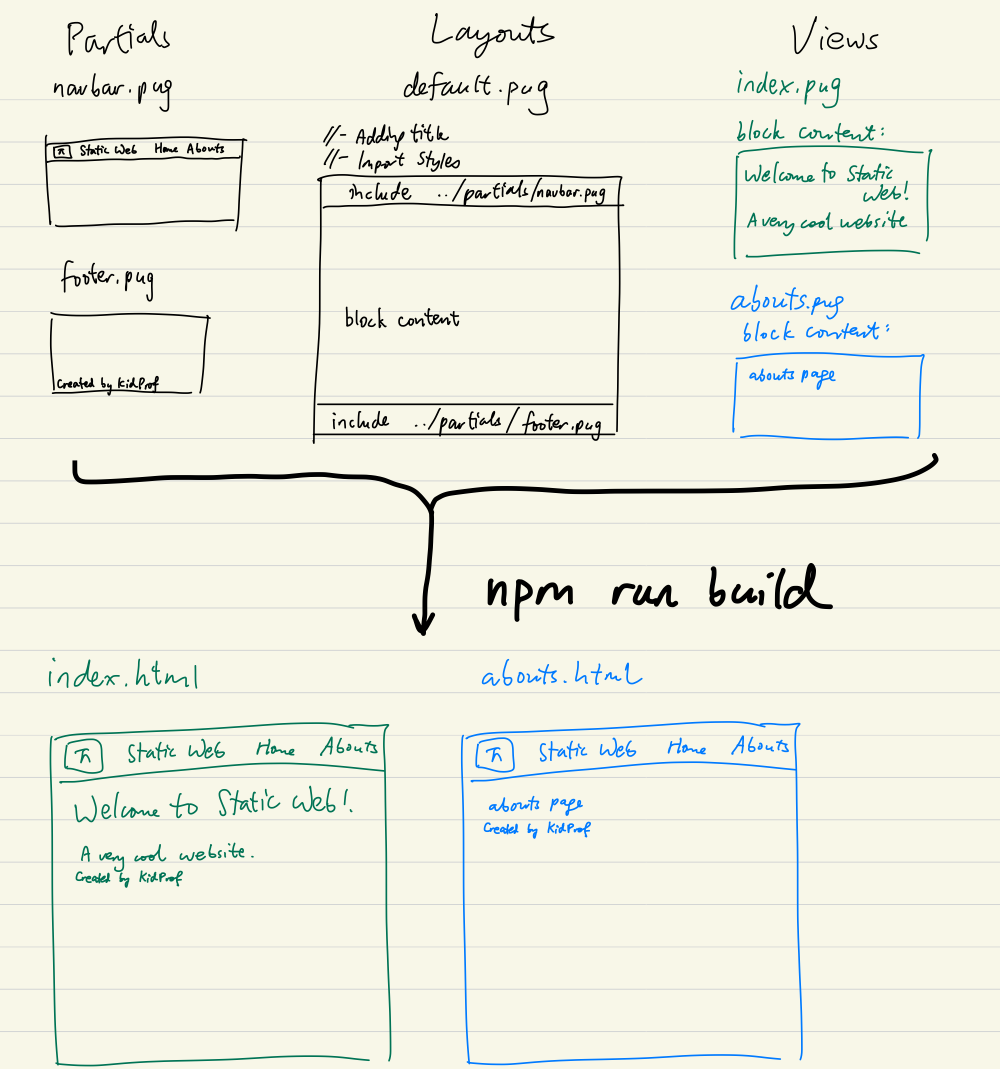
\includegraphics[width=13cm]{images/ch4-puglayouts.png}
\caption{Overview on how Pug files are translated}
\end{figure}

\section{Styling files}

We will be using less files for styling in place for CSS, which are placed under \texttt{app/styles}. We will call them \textbf{Styling files} in this piece of notes. The \texttt{site.less} file includes all files under the \texttt{app/styles/site} folder, \textbf{remember to add the file to \texttt{site.less} whenever you are creating a new less file}. 

The files under the \texttt{site} folder should be where you write the styles. By convention, \texttt{layout.less} should contain styles that is used in all/ multiple pages; \texttt{variables.less} should contain all variables; and other files should contain styles that is only used in the page with the same name as the style file. This is just a convention but not a rule, there is nothing to enforce it until \cref{sec:confinestyles}.

When we run \texttt{npm run build}, the styles got translated into CSS and put into a single file \texttt{docs/styles/site.css}. The stylesheet is imported into all HTML files in line 18 of \texttt{layout.pug}.

\section{Images}

Place all the images or other assets you need for the website under \texttt{\textbf{app}/images} folder. Do not put them inside \texttt{dist}! We will discuss the reasons for that in the next section. 

\section{Website generation}
\label{sec:webgen}
We kept mentioning \texttt{npm run build} as if it is some sort of magic, now it's time to look a little bit closer.

\subsection{\texttt{package.json}}

This file contains basic information about our project (change the name and description if you like). What is more important is the dependencies and the devDependencies, it tells what \texttt{npm}\footnote{stands for Node Package Manager} what libraries you need to run this project, it is written by me, so all you have to do is to run \texttt{npm install} (what you did already in chapter 1), and it knows what to install for you, without the need of you specifying what to install.

Also the scripts section specifies what will be run on \texttt{npm run ...}, from the line \texttt{"build": "gulp build"}, it means the command \texttt{gulp build} will be run when we run \texttt{npm run build}. More in \cref{sec:gulpfile}.

\begin{lstlisting}[language=]
{
  "name": "static-web-sandbox",
  "version": "2.0.0",
  "description": "A very cool website.",
  "dependencies": {
    "gulp": "^4.0.0"
  },
  "devDependencies": {
    "@babel/core": "^7.2.0",
    "@babel/preset-env": "^7.2.0",
    "gulp-babel": "^8.0.0",
    "gulp-changed": "^3.2.0",
    "gulp-eslint": "^5.0.0",
    "gulp-imagemin": "^5.0.3",
    "gulp-less": "^4.0.1",
    "gulp-pug": "^4.0.1",
    "less-plugin-autoprefix": "^2.0.0"
  },
  "scripts": {
    "test": "echo \"Error: no test specified\" && exit 1",
    "build": "gulp build"
  },
  "license": "ISC"
}
\end{lstlisting}

\subsection{\texttt{node\textunderscore modules} folder}

This folder is automatically generated when you run \texttt{npm install}.\footnote{To verify, remove this folder using \texttt{rm -rf node\textunderscore modules} and run \texttt{npm install} again.} It contains the library files you need to run this project, the project would not run without this folder. \textit{You do not need to edit this file at all.}

\subsection{\texttt{package-lock.json}}

This is an automatically generated file, it outlines in detail which version of the dependencies are installed. It automatically updates when you run \texttt{npm install}. \textit{You do not need to edit this file at all.}

\subsection{\texttt{gulpfile.js}}
\label{sec:gulpfile}

This file is responsible for the translation process. As you can see, the task \texttt{pug} translates each \texttt{.pug} file under \texttt{app/templates/views} to HTML files and put them under \texttt{docs}. Similar translation happens for less files. The JavaScript files, images and fonts are copied to the \texttt{docs} folder.

Finally, the task \texttt{build} runs all the above commands. Therefore, \texttt{gulp build} does what is is supposed to do. \textit{You do not need to edit this file at all.}

\begin{lstlisting}[language=JavaScript]
// gulpfile.js
...

//pug to html conversion
gulp.task('pug', function(){
  return gulp.src("app/templates/views/*.pug")
  .pipe(changed("docs/")) //pipe files only if changed 
  .pipe(pug({pretty:true})) //pug to html
  .pipe(gulp.dest('docs/'));
});

//less to css conversion
gulp.task('styling', function(){
  return gulp.src("app/styles/site.less")
  .pipe(changed("docs/styles")) //pipe files only if changed 
  .pipe(less({
    plugins: [autoprefix]
  })) //less to css
  .pipe(gulp.dest('docs/styles'));
});

gulp.task('js',function(){ ... });
gulp.task('imagecopy',function(){ ... });
gulp.task('fontcopy',function(){ ... });

gulp.task('build',gulp.series('js','pug','styling','imagecopy','fontcopy'));

\end{lstlisting}

\subsection{\texttt{docs} folder}

This folder is automatically generated when you run \texttt{run build}.\footnote{To verify, remove this folder using \texttt{rm -rf docs} and run \texttt{npm run build} again.} It is the output folder of the whole project, you can directly open the HTML files inside the folder. You should upload this folder to web servers in order to host it.
\textit{You do not need to edit this file at all.}
\vspace{6mm}

\textbf{IMPORTANT: Do NOT edit anything in the \texttt{docs} folder. Changes will be overwritten when you run \texttt{npm run build} again.}

\subsection{\texttt{.gitignore}}
\label{sec:gitignore}

Because the \texttt{node\textunderscore modules} folder and the \texttt{docs} folder can be automatically generated on your own local machine. There is no need to put these onto GitHub. The \texttt{.gitignore} file lets you state the files and folders that you do not want to push to GitHub. It includes the two folders I have mentioned, and some others that are out of our scope.

\begin{figure}[h]
\centering
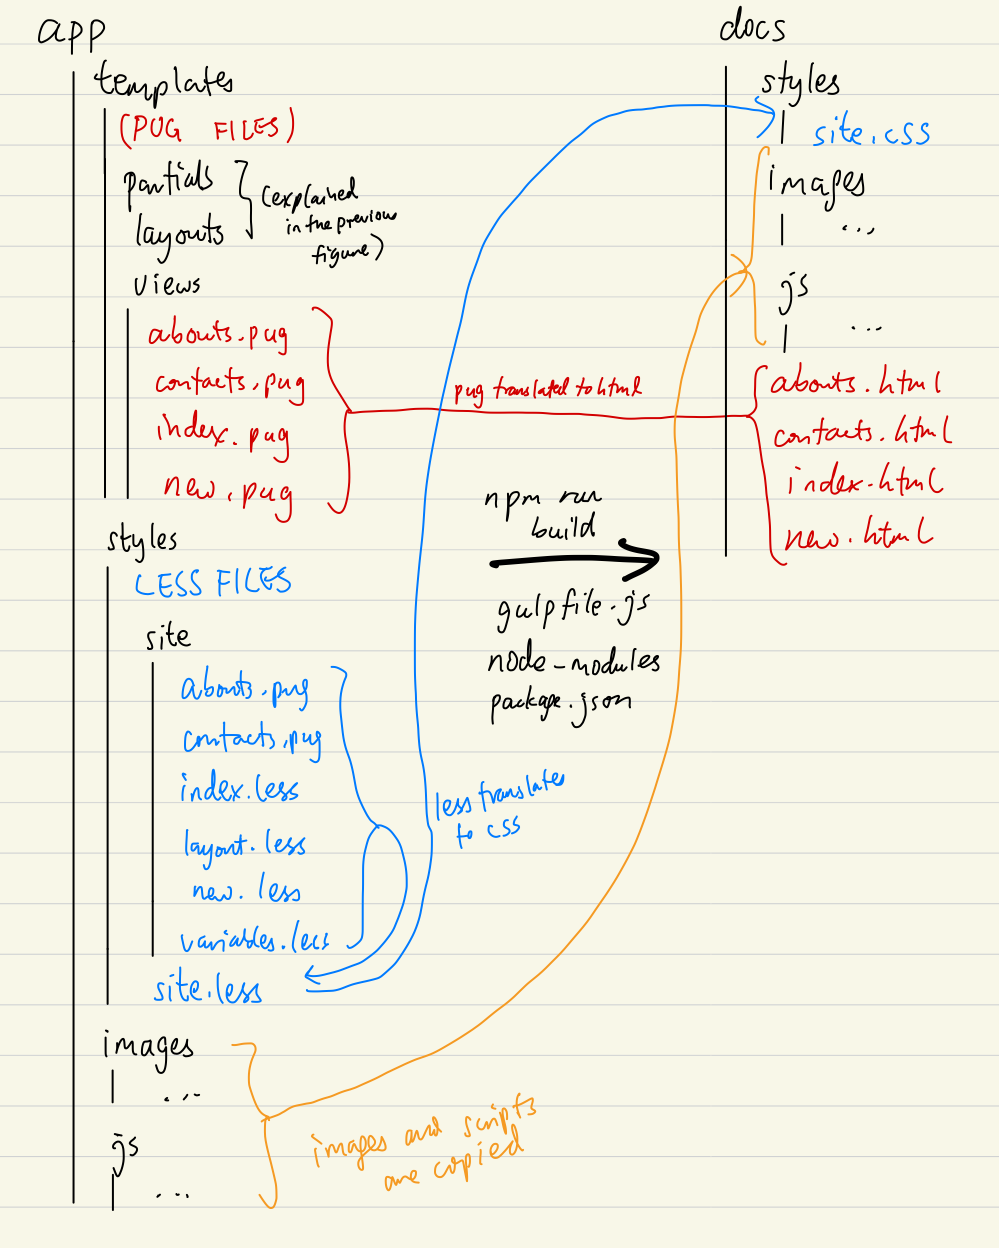
\includegraphics[width=15cm]{images/chn6-full-translation.png}
\caption{Overview of the translation process}
\label{fig:createnewrepo}
\end{figure}

\section{Other files}

\subsection{\texttt{README.md}}
\label{sec:readme}

This file serves as a documentation. It will be displayed on GitHub. You should write a description of your project, and how to install and use it in here. The syntax is a bit weird, refer \href{https://docs.github.com/en/get-started/writing-on-github/getting-started-with-writing-and-formatting-on-github/basic-writing-and-formatting-syntax}{here}\footnote{Link: \url{https://docs.github.com/en/get-started/writing-on-github/getting-started-with-writing-and-formatting-on-github/basic-writing-and-formatting-syntax}} if you want to write your own README.

\subsection{\texttt{.eslintrc}}

\textit{Of less importance}
\vspace{6mm}
This file stores the JavaScript settings and version we are using, so as to check for syntax errors when copying JavaScript files from \texttt{app} to \texttt{docs}. \textit{You do not need to edit this file at all.}

\chapter{Styling}
\label{sec:ch6}

We have wrote the contents for our abouts page in the previous chapter. Now let's make it look prettier.
\vspace{6mm}

Less is used in place of CSS, to provide syntactic sugars\footnote{"Syntactic sugar" is a term for syntax changes in computer programming which make it easier for humans to code.} for us to make our lives easier, including nested styles and variables. 

Note that all knowledge you have learnt for CSS can be transferable to Less, because Less is a superset of CSS. However, we will start from scratch for those of you who have not learnt CSS before.

\section{Further Resources (Ch 6)}

I didn't have this piece of notes back when I first learned Less. Here is \href{https://youtu.be/YD91G8DdUsw}{the video}\footnote{Link: \url{https://youtu.be/YD91G8DdUsw}} that I used to learn the basics. 

You could refer to the \href{https://www.w3schools.com/cssref/}{w3schools documentation}\footnote{Link: \url{https://www.w3schools.com/cssref/}} to learn how to use some more styling tools. However, there is no need to understand every CSS style, the common ones are listed below, and you can google search for the uncommon ones. :)

\section{Referencing elements using classes and IDs}

In this section we will investigate ways to reference the elements we created in the Pug files, so that we can add styles for them.

The easiest way is to reference them using tags, the style below applies to all \texttt{h1} tags in the whole web page. Each style is followed by a semi-colon, and curly braces are used to surround all the styles for the same tag.

\begin{lstlisting}[language=pug]
h1{
    color: red;
}
\end{lstlisting}

However, making all the \texttt{h1} tags red is not usually what we want. To style for specific elements, we would add a class or an ID to the element in the pug file, then reference the class or ID in our less file.

For example, referring to the code from the \hyperref[sec:classesids]{previous chapter}, we can write styles to enlarge and bold some information on the reference book.

\begin{lstlisting}[language=pug]
//- templates/styles/site/abouts.less
.large-text{
    font-size: 1.25rem;
}
\end{lstlisting}

Spaces when specifying the elements for styling means "inside". For example, the following style will affect all \texttt{h3} tags (where there is only one) \textbf{inside} the \texttt{\#quote} div.

\begin{lstlisting}[language=pug]
//- templates/styles/site/abouts.less
#quote h3{
    text-align: center;
    font-style: italic;
}
\end{lstlisting}

We would explain the effect and syntax of different styles in detail in later sections. The difference between using IDs and classes would be explained in the \hyperref[sec:nestedstyles]{nested styles session}.

\section{Text}

\subsection{Text colour}

This changes the colour of the text. Use the \texttt{color}\footnote{Sorry it has to be American spelling :(} keyword, followed by a colon, then specify your colour before finishing off with a semi-colon.

The colour can be specified in \href{https://www.rapidtables.com/web/color/RGB_Color.html}{RGB colour codes}\footnote{Choose your colour: \url{https://www.rapidtables.com/web/color/RGB_Color.html}}, e.g. \texttt{\#FFFFFF} indicates white. \href{https://www.w3.org/wiki/CSS/Properties/color/keywords}{Common colours}\footnote{Full list of "common" colours: \url{https://www.w3.org/wiki/CSS/Properties/color/keywords}} can be specified in text for your convenience, as shown in the previous section.

\begin{lstlisting}
//- templates/styles/site/abouts.less
.blue-text{
    color: #00F; //equivalent to #0000FF
}
\end{lstlisting}

\subsection{Text alignment}

\texttt{text-align} sets the alignment of text. It accepts values \texttt{left} (default), \texttt{center}\footnote{Note the American spelling}, \texttt{right}, and \texttt{justify}\footnote{Sometimes \texttt{justify} might not work very well, if so just use \texttt{left} instead.}

\begin{lstlisting}[language=pug]
//- templates/styles/site/abouts.less
#quote p{
    text-align: right;
}
\end{lstlisting}

\subsection{Font size}

Use the \texttt{font-size} keyword. The interesting thing here is the unit. \texttt{rem} is the ideal unit for text, margins and paddings.\footnote{The reason behind is confusing, refer to \url{https://engageinteractive.co.uk/blog/em-vs-rem-vs-px} if interested.} Normal text should have a font size of 1 rem. Therefore, 1.25rem can be used to indicate a slightly larger text but not overwhelmingly large.

\begin{lstlisting}[language=pug]
//- templates/styles/site/abouts.less
.large-text{
    font-size: 1.25rem;
}
\end{lstlisting}

\subsection{Bold and italic}

\texttt{font-weight: bold;} makes the text bold while \texttt{font-style: italic;} makes the text italic. There is nothing to explain here, but I would like to stress that it is unnecessary to remember every CSS styles by heart. Whenever I need to make some text italic, which is seldom the case, I would search "italic css" and \texttt{font-style: italic;} would pop up. Moreover, there are other alternatives such as using HTML tags \texttt{i} and \texttt{b}.

\section{Positioning}

\subsection{Width and height}
\label{sec:width}

Set the width/ height of a certain element, usually an image. You can either specify it in pixels, or more interestingly, in percentage with respect to the screen. Setting width to be 100\% can be useful when paired with the grid system is quite a nice combo.

\begin{lstlisting}[language=pug]
//- see how it would look like...
#bookofnumbers{
    width: 100%;
    height: 150px;
}
\end{lstlisting}

\subsection{Grid system}
\label{sec:grid}

The grid system is provided by \href{https://getbootstrap.com/docs/5.2/layout/grid}{Bootstrap}\footnote{Full documentation: \url{https://getbootstrap.com/docs/5.2/layout/grid}}. The idea is to split the screen into 12 equal width columns. Then we allocate different number of columns to each element based on the screen size.

There are 6 screen sizes, \texttt{xs}, \texttt{sm}, \texttt{md}, \texttt{lg}, \texttt{xl}, \texttt{xxl}.

We need to surround all elements involved in the grid system with a \texttt{.row} class. To declare number of columns for each screen size, we use \texttt{col-<screensize>-\hfill \break <no.ofcolumns>} (except for xs screens you must not add \texttt{-xs}\footnote{This is Bootstrap's way of reminding us that they employ the "mobile first" principle}). For example, \texttt{.col-12.col-sm-12.col-md-6.col-lg-4.col-xl-3.col-xxl-3} means that the element would occupy the whole screen when the screen is an xs or small screen; half of medium screen, 1/3 of large screens, and 1/4 of xl or xxl screens. Now we would add this style to the abouts page Pug file. Making the reference book info section and the book image side by side when the screen is large enough. The number of columns occupied by the text increases as screen size increases so that the book image is always aligned to the right. (by making the total number of occupied columns adding up to 12)
\vspace{6mm}

\begin{lstlisting}[language=pug]
//- templates/views/abouts.pug
.row
    .col-12.col-sm-12.col-md-6.col-lg-8.col-xl-9.col-xxl-9
        ul
            li.large-text Book name: The Book of Numbers
            li Author: Tim Glynne-Jones
            li Publisher: Arcturus Publishing Limited
            li.large-text Project name: "Numbers are Fun!"
            li.large-text.blue-text Topics chosen: 9, 11, 30, 365.25
        a(href="#self-intro") Back to top
    .col-12.col-sm-12.col-md-6.col-lg-4.col-xl-3.col-xxl-3
        img#bookofnumbers(src="images/bookofnumbers.jpg")
        p.blue-text The Book of Numbers
\end{lstlisting}

\begin{lstlisting}[language=pug]
//- templates/styles/site/abouts.less
#bookofnumbers{
    width: 100%;
}
\end{lstlisting}

There will be more applications of the grid system when \hyperref[sec:cards]{implementing cards in the next chapter.}
\subsection{Flexbox}

Sometimes you would like to position an unknown number of elements, or a number that is not divisible by 12, then using the grid system might not be a good idea. We can use flexbox in these scenario. It is \href{https://css-tricks.com/snippets/css/a-guide-to-flexbox/}{well documented}\footnote{Documentation: \url{https://css-tricks.com/snippets/css/a-guide-to-flexbox/}} with clear illustrations. And here is an \href{https://flexboxfroggy.com/}{interactive tutorial}\footnote{Tutorial: \url{https://flexboxfroggy.com/}}. In order to use all the styles listed in there, you first have to surround the elements involved with an element with the style \texttt{display: flex;}, bring all the elements within it to the "flex world".

It could be hard to get right at first, I recommend using the browser developer mode to experiment more with flexbox, add the related stles to different layers of elements and see which ones works. 

Learning the concept of flexbox is useful when building apps.

\section{Margins and paddings}
\label{sec:margin}

\subsection{Background colour}

\texttt{background-color} sets the colour of the background. The default value is \texttt{transparent}. It is important to distinguish between a white background and a transparent background. More on background colour in \hyperref[sec:margin]{the section on margin and paddings}.

\begin{lstlisting}[language=pug]
#self-intro{
    background-color: #777; //#777 is equivalent to #777777
}
\end{lstlisting}

\subsection{Margins}

\subsection{Paddings}

\subsection{Borders}

\section{Other styles}

\subsection{Bold}

\subsection{Italics}

\section{Nested styles}
\label{sec:nestedstyles}

\subsection{Styling priority}

\section{Using variables}
\chapter{Git (II) - Collaborating With Others}
\label{sec:git2}
% Old Ch. 8

\textit{Advanced Chapter}
\vspace{6mm}

The commands introduced in \cref{sec:ch3} is only enough for working alone, mainly the normal \texttt{git add .; git commit -m "message"; git push} procedure. Things are slightly more hectic when you have more than one person working together in the same repository concurrently. 

\section{The ideal situation}

To make things simple, we can add a restriction that only one user can work on the project at a time. After someone has finished working, they push their code to GitHub. Then all other people would get the latest code from GitHub and download it to their local device using \texttt{git pull} before they start working on their part of the code. 

\begin{figure}[h]
\centering
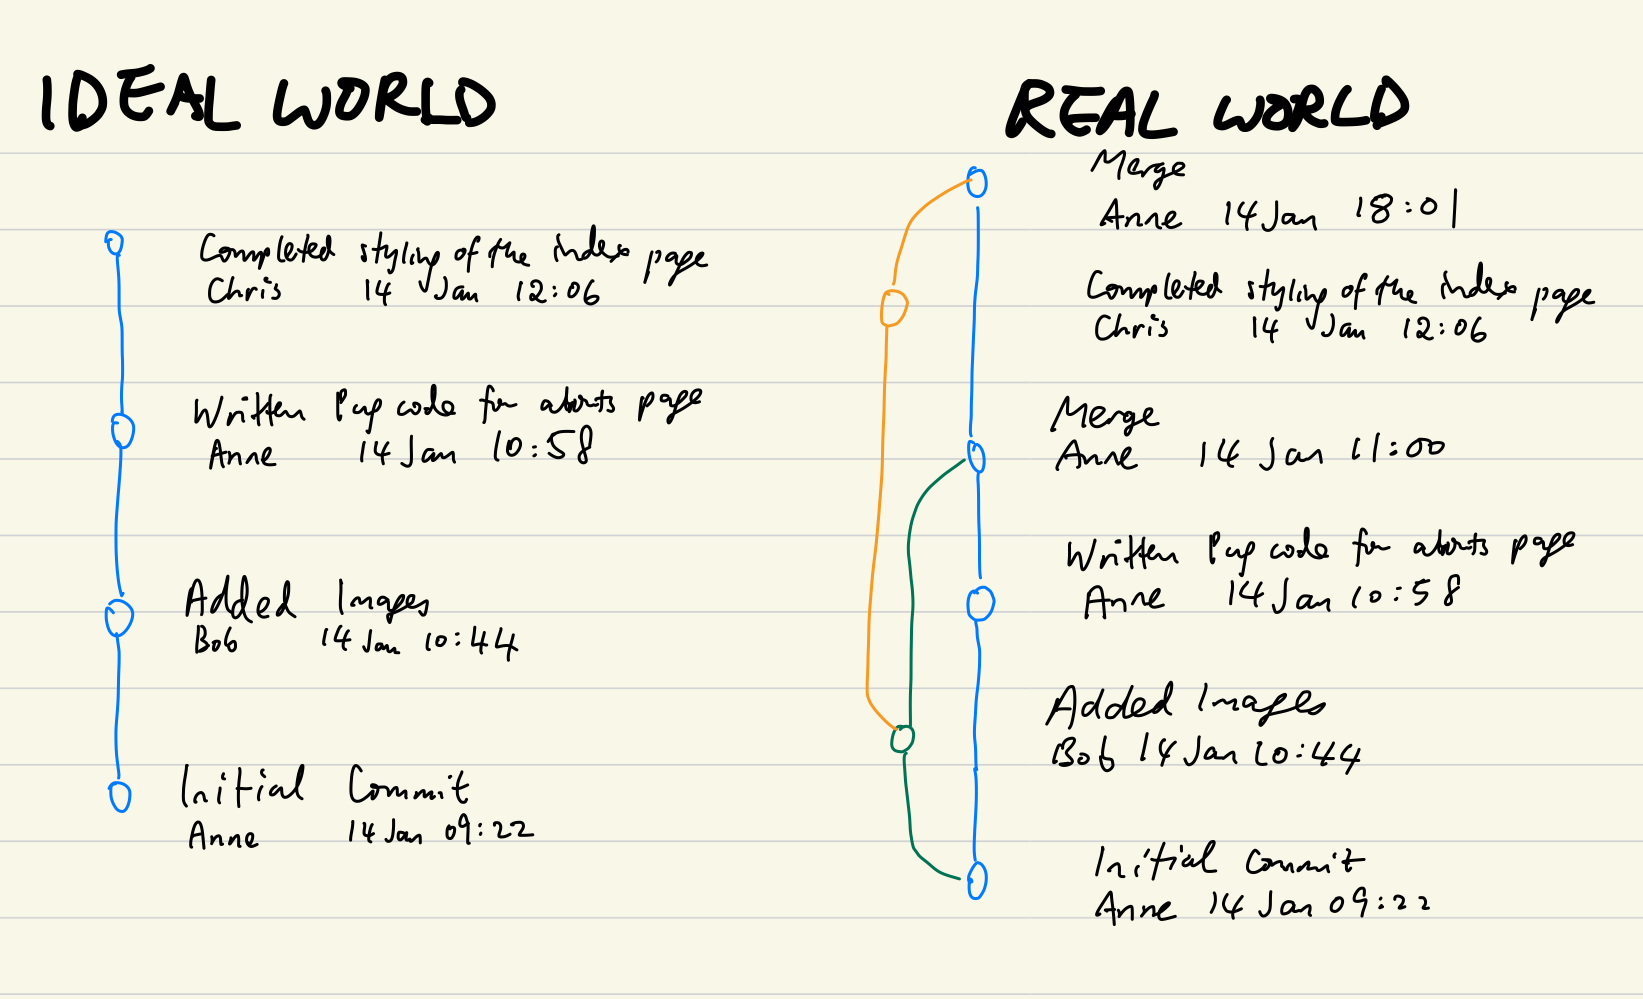
\includegraphics[width=15cm]{images/ch8-messy-git-world.png}
\caption{Messy world of Git}
\end{figure}

Of course, the above method is impractical, what we actually want is multiple people being able to work on the code at the same time. Or sometimes people simply forget to \textbf{pull} (fancier word for download) the latest version of the code before they start working. We have to accept the fact that our \textbf{commit history} (fancier term for edit history) is not a straight line and diversions are unavoidable, just like our lives.\footnote{For fun: life is not a straight line \url{https://amandalinehan.com/life-is-not-a-straight-line/}} We will discuss git commands and techniques that can help you to work with different people in this chapter.

\section{Know what others are doing}
\label{sec:gitpull}

Git operates offline on its own on your local machine unless you request it to look at the changes on GitHub. (the cloud) 

As indicated in the previous section, we use \texttt{git pull} to download the updates of the code from GitHub to our local machine. Pull is another word for download.

Note the distinction between \texttt{git pull} and \texttt{git clone} (see \cref{sec:gitclone}). \texttt{git clone} is to copy the repository to your local device, it is only used to download the code initially. \texttt{git pull} is used for subsequent downloads, which aims to update the local code with newest changes.

But sometimes, you just want to see what's made by others before pulling the code. You can do so by \texttt{git fetch}. It updates the local machine what's going on in the GitHub repository, but will not download any code, you can view the updates using one of the visualisation tools in \cref{sec:sublime}.

Visualisation tools are super useful throughout this chapter as they let you see what's going on on different branches in a fashion that is similar to my illustrations.

\begin{figure}[h]
\centering
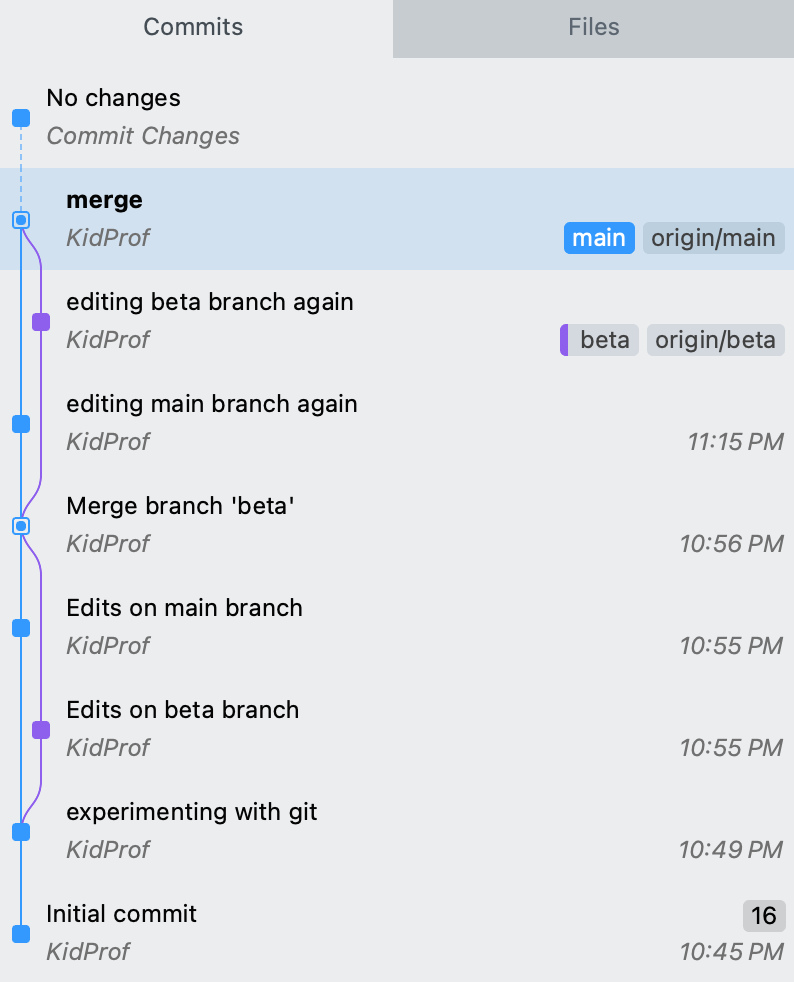
\includegraphics[width=7cm]{images/ch8-sublimemerge.png}
\caption{What sublime merge shows following the tutorial up to \cref{sec:mergeconflict}}
\end{figure}

\section{Branching out}
\label{sec:branch}

We use branches to maintain different versions of the same project. 

\subsection*{Switching between branches}

Creating a new branch using \texttt{git checkout -b} followed by the branch name you want. In the example below, we switched from main branch to our newly created beta branch. The newly created branch has the same contents as the branch you switched from.

To switch to an existing branch, we use \texttt{git checkout}. Note that for subsequent switches to the beta branch you don't need \texttt{-b} anymore, since the beta branch was created already and it is now an existing branch.

\begin{lstlisting}[language=bash]
# KidProf in ~/code/git-tutorial on git:main x [22:38:58]
$ git checkout -b beta
Switched to a new branch 'beta'

# KidProf in ~/code/git-tutorial on git:beta x [22:39:12]
$ git checkout main
Switched to branch 'main'

# KidProf in ~/code/git-tutorial on git:main x [22:40:58]
$ git checkout beta
# Note no need -b here as beta is now an existing branch
Switched to branch 'beta'

# KidProf in ~/code/git-tutorial on git:beta x [22:44:10]
\end{lstlisting}

In Git Bash and MacOS zsh (see \cref{sec:iterm} for set up) you can see the branch that you are currently in.

\subsection*{Making edits}

Switching between branches is not particularly interesting for now, because both branches have the same content, so let's now change that.

In the beta branch, we can try editing a random file. Ideally mention something about the beta branch for easier recognition.

\begin{lstlisting}[language=pug]
//- app/templates/views/index.pug
extends ../layouts/default

block content
	.container
		h1 Welcome to Static Web!
		br
		p A very cool website.
		p This web is made for tutorial purposes.
		p Edits on beta branch in index page.  
		    //- ^new line
\end{lstlisting}

Commit your changes, using the three steps mentioned in \cref{sec:gcmsg}

\begin{lstlisting}[language=bash]
$ git add .
$ git commit -m "edits on beta branch"
$ git push
\end{lstlisting}

You might need to run \texttt{git push --set-upstream origin beta} instead because this is the first push of a new branch. 

Then let's switch back to main branch using \texttt{git checkout main}. Open the file you have modified in the beta branch, you will realise your edits are gone!

This is because we are now at the main branch, and you were making edits on the beta branch instead. Changes on one branch will not affect other branches, this is how you are able to maintain different versions of the same project.

We can make further experimentation with branches by making edits in the main branch also. I deliberately made edits to a different file, the reason will become apparent in the next section.

\begin{lstlisting}[language=pug]
//- app/templates/views/abouts.pug
extends ../layouts/default

block content
	.container
		p abouts page
		p Edits on main branch in abouts page.
		    //- ^new line
\end{lstlisting}

\begin{lstlisting}[language=bash]
$ git add .
$ git commit -m "edits on main branch"
$ git push
\end{lstlisting}

Now you can switch back and forth between the two branches and see that the contents are different.

\begin{figure}[h]
\centering
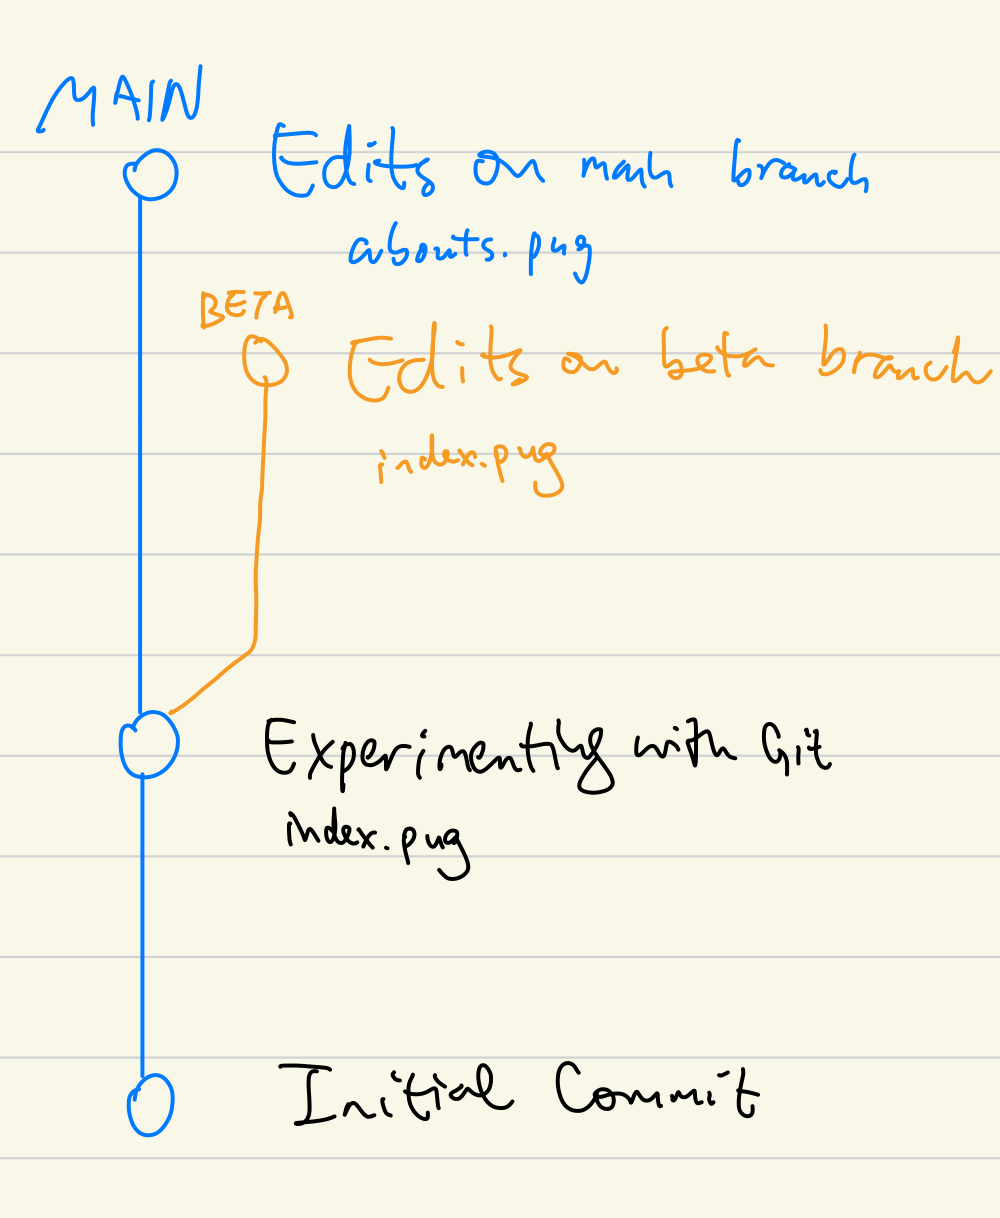
\includegraphics[width=7cm]{images/ch8-branching.png}
\caption{Visualising the two branches created}
\end{figure}

\subsection*{Uses of branches}
Yes we use branches to maintain different versions of the same project. A common practice will be each employee of a company would work on their own branch named after their name (e.g. dev-kidprof), so that they can work on their own tasks without interfering with others.

However, we only want one version at the end, the version that you publish to the public. To achieve this, all the employees' branches will be \textbf{merged} (see next section) back to the main branch. The main branch usually is the final product of the project and it should be relatively error free because all known issues should be resolved before merging code from other branches to the main branch.

\section{Merging}
\label{sec:merge}

\subsection{Merging without conflicts}

We will try to merge the beta branch into the main branch (i.e. apply the changes in beta branch to the main branch)

We can do so by first checking out to the main branch, the branch that you want to merge into.

\begin{lstlisting}[language=bash]
$ git checkout main
\end{lstlisting}

Then run the command \texttt{git merge}, to merge the beta branch into the main branch.

\begin{lstlisting}[language=bash]
$ git merge beta
\end{lstlisting}

A command line text editor may pop up, we do not need to modify anything. So we can just type \texttt{:wq} then tap enter to quit the text editor and save. For more information on how to control the command line text editor, refer to \cref{sec:vim}.

When you check your code, your edits in both the index page and abouts page should be there. :)

Finally, push our merge to GitHub with \texttt{git push}.
\vspace{6mm}

If you want your beta branch to obtain the updates from the main branch, we can do the same for beta branch, that is:

\begin{lstlisting}[language=bash]
$ git checkout beta
$ git merge main
$ git push
\end{lstlisting}

\begin{figure}[h]
\centering
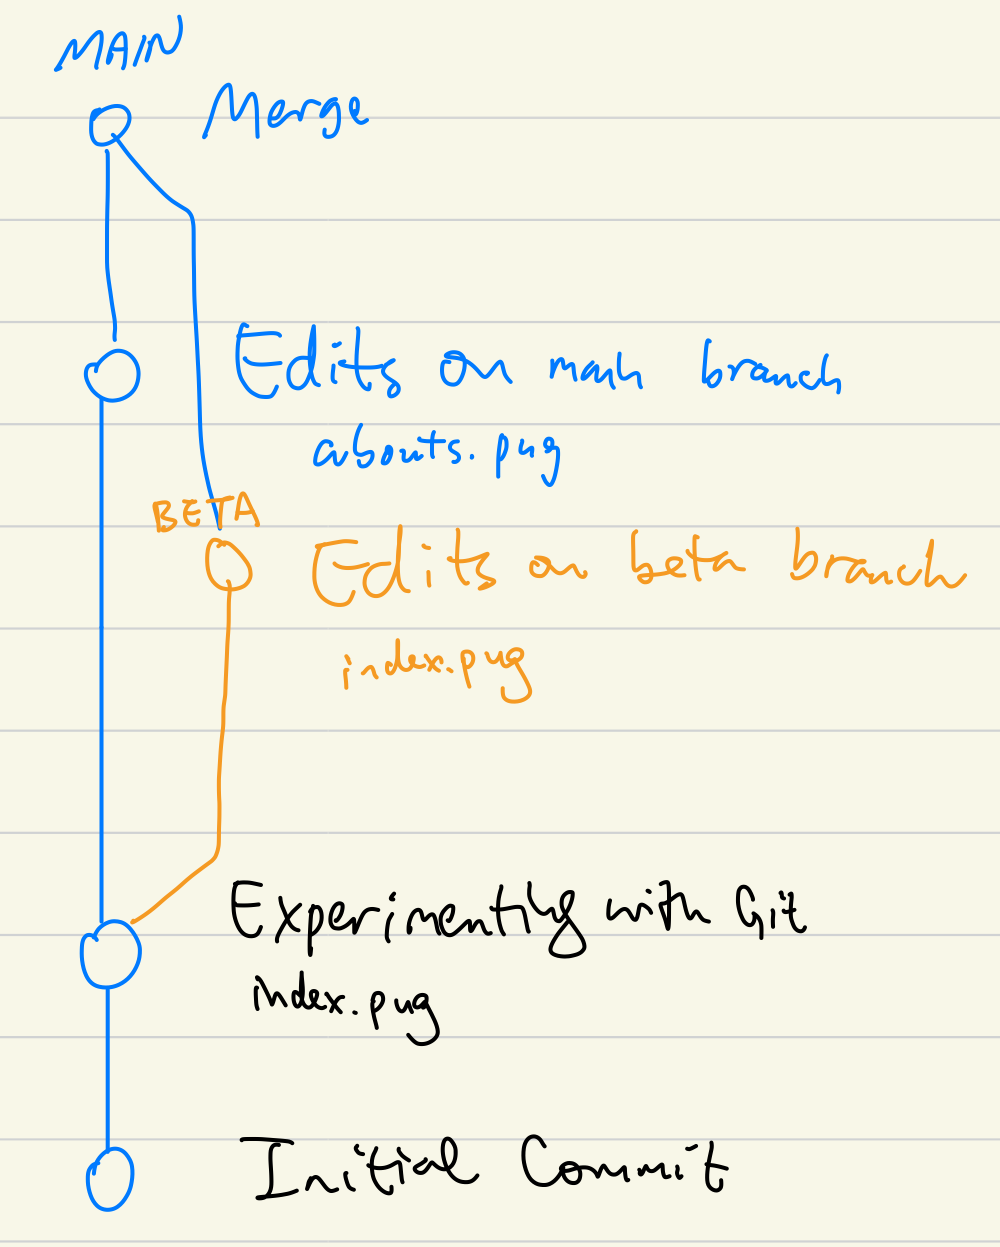
\includegraphics[width=7cm]{images/ch8-merge-safe.png}
\caption{Visualising the merge}
\end{figure}

\subsection{Merge conflicts}
\label{sec:mergeconflict}
The merge just now seems a bit too easy, that is because the two branches edited different files. The merging process would be more interesting when both branches edit the same part of the file. The following illustrates an example.
\vspace{6mm}

We first go to main branch and add a new line in \texttt{index.pug}.

\begin{lstlisting}[language=bash]
$ git checkout main
\end{lstlisting}

\begin{lstlisting}[language=pug]
//- app/templates/views/index.pug
...
p This web is made for tutorial purposes.
p Edits on beta branch in index page.
p New line on main branch. //- new line
\end{lstlisting}

\begin{lstlisting}[language=bash]
$ git add .
$ git commit -m "editing main branch again"
git push
\end{lstlisting}

Then we go to the beta branch and do the same. You will see the edits you have made for the abouts page (if you have not merged the main branch back into the beta branch) and also the edits you have made just now are missing, that is because we are in a different branch.

\begin{lstlisting}[language=bash]
$ git checkout beta
\end{lstlisting}

\begin{lstlisting}[language=pug]
//- app/templates/views/index.pug
...
p This web is made for tutorial purposes.
p Edits on beta branch in index page.
p New line on beta branch. //- new line
\end{lstlisting}

\begin{lstlisting}[language=bash]
$ git add .
$ git commit -m "editing beta branch again"
$ git push
\end{lstlisting}

Then we go back to the main branch and try to merge the beta branch into the main branch.

\begin{lstlisting}[language=bash]
$ git checkout main

# KidProf in ~/code/git-tutorial on git:main o [23:28:42]
$ git merge beta
Auto-merging app/templates/views/index.pug
CONFLICT (content): Merge conflict in app/templates/views/index.pug
Automatic merge failed; fix conflicts and then commit the result.
\end{lstlisting}

When you run \texttt{git status}, you can see it tells you that both branches modified \texttt{index.pug}.

\begin{lstlisting}[language=bash]
$ git status
On branch main
Your branch is up to date with 'origin/main'.

You have unmerged paths.
  (fix conflicts and run "git commit")
  (use "git merge --abort" to abort the merge)

Unmerged paths:
  (use "git add <file>..." to mark resolution)
	both modified:   app/templates/views/index.pug
\end{lstlisting}

When you open VS code, you may see VS code provides a nice interface to help you to fix the merge conflict. (\cref{fig:vscodemergeconflict})

\begin{figure}[h]
\centering
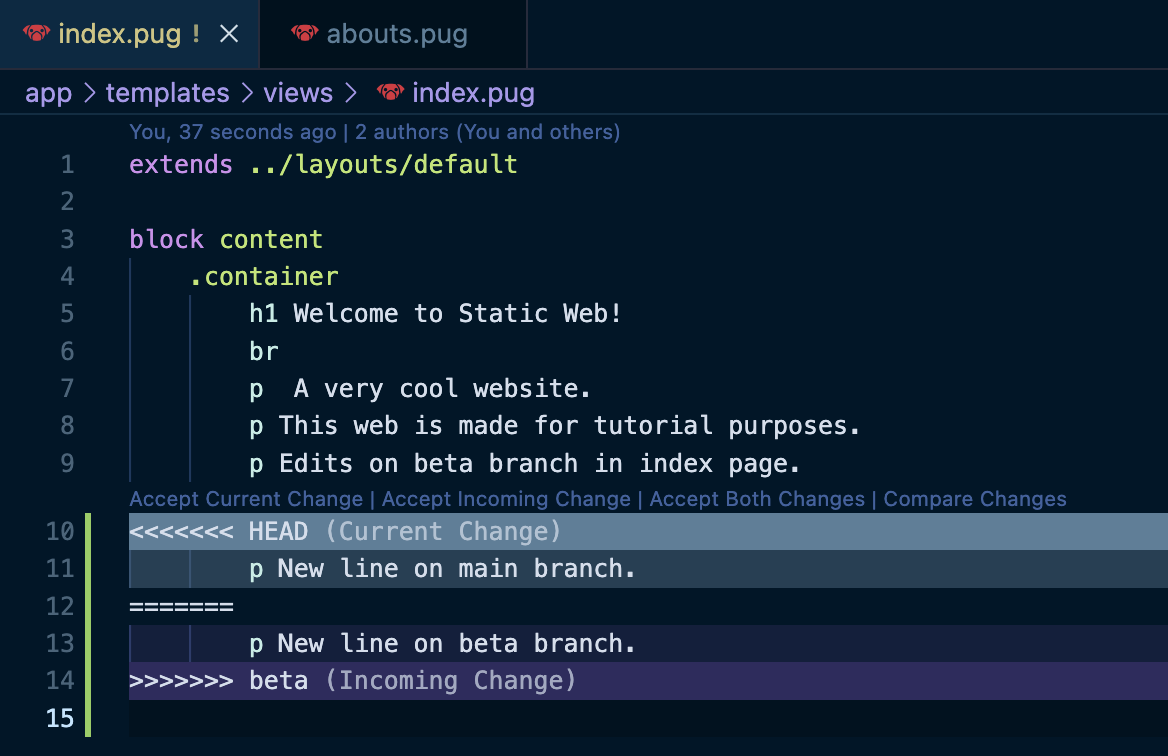
\includegraphics[width=10cm]{images/ch8-merge-conflict-vscode.png}
\caption{VS Code's interface to help you solve merge conflicts}
\label{fig:vscodemergeconflict}
\end{figure}

But let's analyse it in the hardcore way first, you shouldn't need any more additional tools to fix a merge other than a plain text editor. 

\begin{lstlisting}[language=pug]
extends ../layouts/default

block content
	.container
		h1 Welcome to Static Web!
		br
		p  A very cool website.
		p This web is made for tutorial purposes.
		p Edits on beta branch in index page.
<<<<<<< HEAD
		p New line on main branch.
=======
		p New line on beta branch.
>>>>>>> beta
\end{lstlisting}

As you can see, it uses arrows to indicate the area of the conflict, and listed both versions separately with equal signs in the middle. What you should do is merge the changes of the two versions and remove the arrows and equal signs, and Git will regard that conflict as fixed. 

In this example, let's change it to \texttt{New line on both branches.} Remove all the arrows and equal signs (more on what to merge in the FAQs below).

\begin{lstlisting}[language=pug]
//- app/templates/views/index.pug
extends ../layouts/default

block content
	.container
		h1 Welcome to Static Web!
		br
		p  A very cool website.
		p This web is made for tutorial purposes.
		p Edits on beta branch in index page.
		p New line on both branches.
\end{lstlisting}

Finally, we just use the daily routine to push our merged code to GitHub. If no errors appear when running \texttt{git add .}, it means you have merged the code successfully.

\begin{lstlisting}[language=bash]
$ git add .
$ git commit -m "merge"
$ git push
\end{lstlisting}

\subsection*{When would there be a conflict when merging?}

When both branches modify the same part of the same file. (If two branches modify different parts of the file, there might not be one if Git recognises that the two edits are far away enough.)

\subsection*{Which changes should I choose when there is a conflict?}
\label{sec:mergefaq}
It heavily depends on the situation! The Git tools provided by VS code may make you think that only changes from one of the branches can be taken and we must discard the other one, this is definitely not the case. The product of the merge should be what you want to be in your project finally. Maybe one of them is more updated, maybe you need to incorporate elements of both changes. For example, one branch may have changed the indentation of a part of the code because they are now put in an if clause, while the other branch may have edited the contents of one of the lines being indented. What you actually want is neither of them, but you need both the indentation change and content change. There is another slightly more elaborate example in the next section.

\subsection*{Is merge conflict bad?}

Not at all, different versions of code would definitely appear as multiple people edit the code in parallel. \texttt{git merge} provides you with a systematic tool to merge the differences and create one single final product. As long as you don't panic and merges the code correctly, aiming at making the final product better and bug free, it is completely fine. 

\section{Merges due to edits on the same branch}
\label{sec:mergesamebranch}

It is not a must for different people to make edits on their own branch, multiple people could be work on the same branch for convenience. But there must only be one most updated version of the branch at a given time on GitHub, so Git will refuse to push your code when somebody else has made edits on the same branch previously that you haven't pulled. 

This is best done using two people, the two people will be Anne and Bob in my example. \footnote{You can sort of simulate that by having two copies of the same project on your device by leaving the current project directory and then running \texttt{git clone $<$url$>$ git-tutorial-2} (but this is not ideal as you may just get yourself confused.)}

This is very similar to the last section, we are also merging two different versions of code, but this time they are from the same branch, that means we must merge it as there must only be one version of the branch at a given time. However, in the previous section, we can delay our merge until whenever we need to.

First, Anne makes some edits in the abouts page in the main branch. 

\begin{lstlisting}[language=bash]
# Anne
$ git checkout main
\end{lstlisting}

\begin{lstlisting}[language=pug]
//- Anne: app/templates/views/abouts.pug
...
p Edits on main branch in abouts page.

h1 Self introduction
ul
	li Anne: Hi I am Anne I love coding.
\end{lstlisting}

\begin{lstlisting}[language=bash]
# Anne
$ git add .
$ git commit -m "added self intro section and Anne's description"
$ git push
\end{lstlisting}

Then Bob makes similar changes, probably he isn't told that Anne has worked on it already.

\begin{lstlisting}[language=bash]
# Bob
$ git checkout main
\end{lstlisting}

\begin{lstlisting}[language=pug]
//- Bob: app/templates/views/abouts.pug
...
p Edits on main branch in abouts page.

h2 Self introduction
ul
	li Bob: Hi I am Bob I love programming.
\end{lstlisting}

As Anne has made some changes earlier, Bob cannot push his code as smoothly.

\begin{lstlisting}[language=bash]
# Bob
$ git add .
$ git commit -m "added self intro section and Bob's description"
$ git push
To github.com:KidProf/git-tutorial.git
 ! [rejected]        main -> main (fetch first)
error: failed to push some refs to 'github.com:KidProf/git-tutorial.git'
hint: Updates were rejected because the remote contains work that you do
hint: not have locally. This is usually caused by another repository pushing
hint: to the same ref. You may want to first integrate the remote changes
hint: (e.g., git pull ...) before pushing again.
hint: See the 'Note about fast-forwards' in 'git push --help' for detail
\end{lstlisting}

Git advises Bob to first pull the code from the main branch. After running \texttt{git pull}, the situation would be the \textbf{same as the previous section}. What need to do depends on whether there are merge conflicts. If there are no merge conflicts, you just need to add commit and push your merge. (Exercise: Try this case on your own with your friends)
\vspace{6mm}

We were told by Git that unfortunately there is a merge conflict at \texttt{abouts.pug}, as you should expect, because both Anne and Bob modified the same part of the abouts page.

\begin{lstlisting}[language=pug]
//- Bob: app/templates/views/abouts.pug
extends ../layouts/default

block content
	.container
		p abouts page
		p Edits on main branch in abouts page.
<<<<<<< HEAD
		h2 Self introduction
		ul
			li Bob: Hi I am Bob I love programming.
=======
		h1 Self introduction
		ul
			li Anne: Hi I am Anne I love coding.
>>>>>>> 484fb78c7ac9f62c53cd8b87529e91d5252a60e9
\end{lstlisting}

We definitely want both of their self introductions in the final product, and we can choose between \texttt{h1} and \texttt{h2} and see which one is more aesthetically pleasing. Let's choose \texttt{h2} for now. Make sure to remove the arrows and equal signs after you have finished. 

\begin{lstlisting}[language=pug]
//- Bob: app/templates/views/abouts.pug
extends ../layouts/default

block content
	.container
		p abouts page
		p Edits on main branch in abouts page.
		h2 Self introduction
		ul
			li Bob: Hi I am Bob I love programming.
			li Anne: Hi I am Anne I love coding.
\end{lstlisting}

Then we just continue with the normal procedure. This is what you should do as well when there are no merge conflicts.

\begin{lstlisting}[language=bash]
# Bob
$ git add .
$ git commit -m "merge"
$ git push
\end{lstlisting}

\begin{figure}[H]
\centering
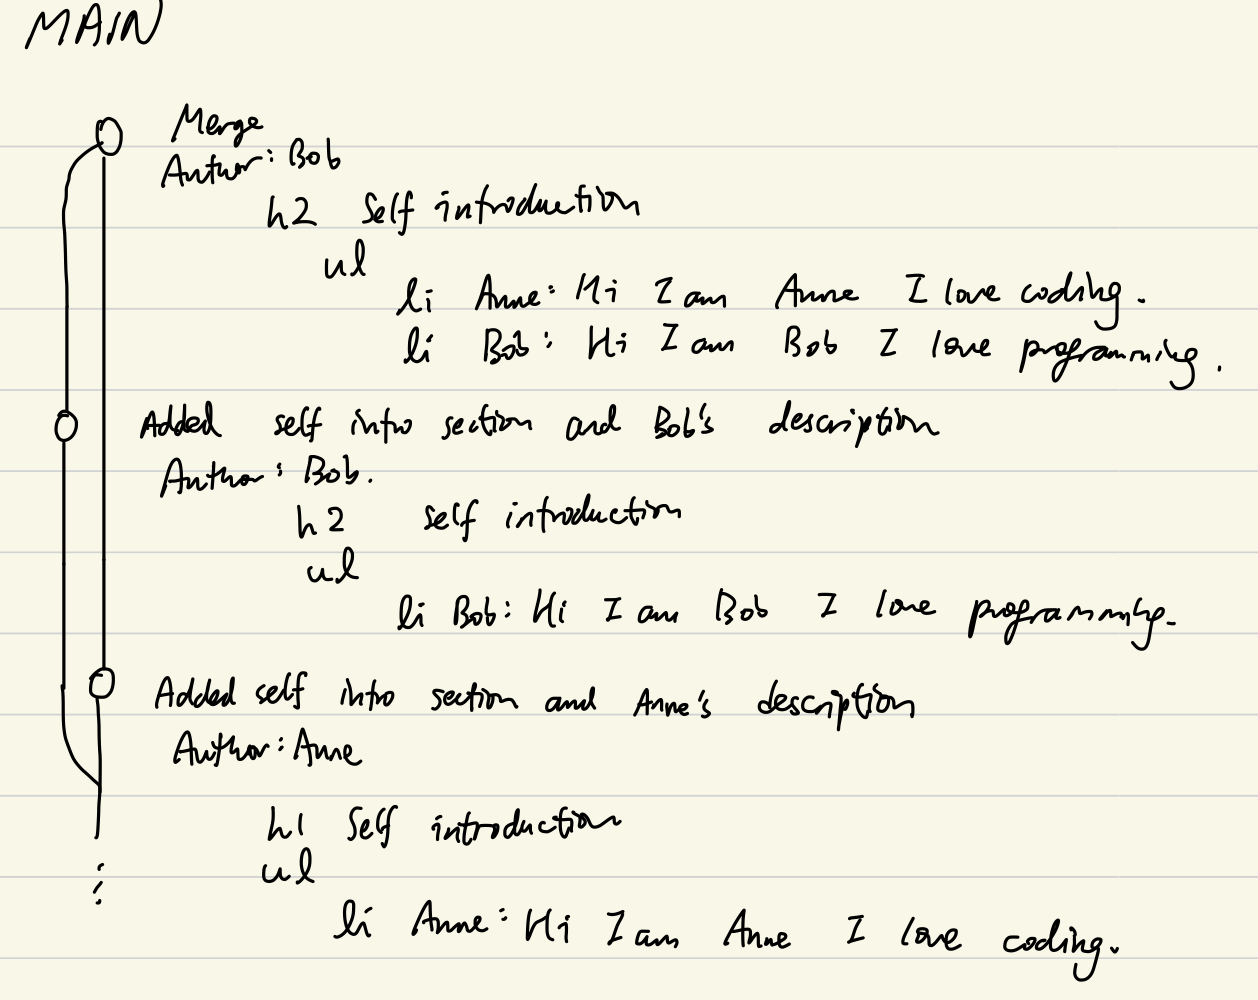
\includegraphics[width=15cm]{images/chn8-same-branch-merge.png}
\caption{Visualising the merge}
\end{figure}

% \section{Stashing}

% \textit{Of less importance}
% \vspace{6mm}

% A temporary local area for you to store your edits. When you think your local edits are useful/ not ready to push but you need to work on other branches immediately. You can temporarily store your code on your local machine using \texttt{git stash}. More information on how to use is in the git commands table below.

\section{Something went wrong?}

The examples in this chapter are quite artificial. However, I hope you are convinced that branching, merging and merge conflicts are unavoidable when working with different people using Git. They might be intimidating at first (especially merge conflict), but what you only need is some practice. 

You can refer to tips in \cref{sec:gitpractice} if there are some errors on Git that you don't know how to fix. To add to the list, another thing you can do if you find it difficult to solve the merge conflict, run \texttt{git merge --abort} to stop the merge, then create a new temporary branch, and push your code there first. Then merge when you feel more comfortable or during lesson time.

\begin{table}[H]
    \centering
    \caption{Table of common Git commands}
    \vspace{6mm}
    \begin{tabular}{|m{7em}|m{23em}|}
        \hline
        \textbf{Command} & 
        Description 
        \\ \hline \hline
        
        \texttt{git status} &
        Displays information about current situation, it might also contain some hints on which command(s) you should run to proceed. (\cref{sec:gcmsg})
        \\ \hline
        
        \texttt{git add .} &
        First step to push your code to GitHub - includes all the changes in the folder to be ready for a commit (\cref{sec:gcmsg})
        \\ \hline
        
        \texttt{git commit -m "message"} &
        Second step to push your code to GitHub - seals and confirms your changes into one chunk, and adds a commit message (\cref{sec:gcmsg})
        \\ \hline
        
        \texttt{git push} &
        Third step to push your code to GitHub - uploads the commit from your local machine to GitHub (\cref{sec:gcmsg})
        \\ \hline
        
        \texttt{git init} &
        Initialises a new Git repository in the current folder on your local machine (\cref{sec:gitinit})
        \\ \hline
        
        \texttt{git clone $<$url$>$} &
        Creates a new folder with the repository name would be created with all the code inside (\cref{sec:gitclone})
        \\ \hline
        
        \texttt{git pull} &
        Downloads the updates of the code from GitHub to our local machine (\cref{sec:gitpull})
        \\ \hline
        
        \texttt{git fetch} &
        Updates the local machine what's going on in the GitHub repository, but will not download any code. (\cref{sec:gitpull})
        \\ \hline
        
        \texttt{git checkout -b $<$branch$>$} &
        Creates a new branch (\cref{sec:branch})
        \\ \hline
        
        \texttt{git checkout $<$branch$>$} &
        Moves to another existing branch (\cref{sec:branch})
        \\ \hline
        
        \texttt{git merge $<$branch$>$} &
        Merges the updates on the specified branch into the current branch. (\cref{sec:merge})
        \\ \hline
        
        % \texttt{git stash -u} &
        % Save current changes, including new (untracked) files (\cref{sec:gitstash})
        % \\ \hline
        
        % \texttt{git stash pop} &
        % Apply the changes you recently saved. (\cref{sec:gitstash})
        % \\ \hline
        
        % \texttt{git stash clear} &
        % Remove all stashes. (\cref{sec:gitstash})
        % \\ \hline
        
    \end{tabular}
\end{table}

\chapter{Pug.js (II) - Use of Variables}
\label{sec:pug2}
% Old Ch. 9


\textit{Advanced Chapter}
\vspace{6mm}

\textit{Not completed yet, as explained in \cref{sec:incompletewarning}}
\vspace{6mm}

\section{Variables}


\section{Interpolation - Having variables in body texts}


\section{Mixins}


\section{Worked Examples}


Now we will demonstrate a few examples that make use of knowledge from chapters 4-7 to style elements conditionally using variables.

\section{Navbar}
\label{sec:navbar}

\section{Confining styles within the page}
\label{sec:confinestyles}

\section{Light and Dark Themes}


\chapter{Misc}
\label{sec:misc}
% Old Ch. 10

\textit{Of less importance}
\vspace{6mm}

\section{Fonts}
\label{sec:fonts}

\textit{Not completed yet, as explained in \cref{sec:incompletewarning}}

\section{Web Hosting}
\label{sec:webhosting}

\textit{Not completed yet, as explained in \cref{sec:incompletewarning}}

\section{Common Errors}

\subsection{Pug: Invalid indentation, you can use tabs or spaces but not both}

This error might appear when you run \texttt{npm run build}.
You can either use tab or 4 spaces to represent indentation in Pug, but it has to be consistent throughout a file. You encounter this error because you sometimes use spaces, sometimes use tabs for indentation in the same file. Solve this error by replacing all tabs with 4 spaces, or vice versa. It is difficult because you can't distinguish them in the text editor. I recommend using the find and replace tool. To insert a tab in the search/ replace box, copy a tab from elsewhere and paste it.

\subsection{npm: Local modules not found}

This error might appear when you run \texttt{npm run build}. It means that the node modules are not installed yet. Run \texttt{npm install} to fix. 

\subsection{Styling: My styles are not appearing}

Check the browser developer tools.

If the styles you have written appears there but crossed out, it means your styles do not have high enough priority, check out \cref{sec:stylingpriority} to see how you can increase the priority of the styles.

If you cannot see the styles you have written, double check the less file to make sure you are referencing the correct element. Also double check if the less file is included in \texttt{app/styles/site.less}

\subsection{My images/ other edits are gone after re-downloading the code from GitHub}

It might because you put your images/ made edits under the \texttt{docs} folder. Remember you must make all edits under the \texttt{app} folder. Things under the \texttt{docs} folder will not be pushed by GitHub and will be overwritten on \texttt{npm run build}.

\section{Optional QOL tools for MacOS}
\label{sec:iterm}
\textit{Of less importance, covered in \href{https://www.youtube.com/watch?v=ZIBEVGrtiVA&list=PLjGmdnqrOKuYXiu7lgG5HW71jPEUd1XCm&index=7}{video 6a of the series}}
\vspace{6mm}

Refer to \href{https://www.youtube.com/watch?v=ZIBEVGrtiVA&list=PLjGmdnqrOKuYXiu7lgG5HW71jPEUd1XCm&index=7}{the video}\footnote{Link: \url{https://www.youtube.com/watch?v=ZIBEVGrtiVA&list=PLjGmdnqrOKuYXiu7lgG5HW71jPEUd1XCm&index=7}}.

Here is an outline on what is installed.
\begin{itemize}
    \item iTerm2 - \url{https://iterm2.com/}
    \item oh my zsh - \url{https://ohmyz.sh/}
    \item Colour theme - \url{https://github.com/MartinSeeler/iterm2-material-design}, follow the documentation in the README and apply the colour theme to your terminal
    \item Changing the theme of oh my zsh by editing the \texttt{.zshrc} file by running \texttt{open .zshrc}. Edit one of the lines to \texttt{ZSH\textunderscore THEME = "ys"} 
    \item tldr pages - \url{https://tldr.sh/}

\end{itemize}

\section{Optional VS Code Plugins}
\textit{Of less importance}
\vspace{6mm}

Refer to the very last section of \href{https://github.com/OscarMui/setup-cheetsheet-macos}{my setup cheetsheet}\footnote{Link: \url{https://github.com/OscarMui/setup-cheetsheet-macos}} (last part works for all operating systems) Not all of them are useful to you, just choose ones that you like.

Here is an outline on something that might be useful. These are the extension IDs, copy and paste them in the search extensions box to find them.

\begin{itemize}
    \item sdras.night-owl (A cooler theme)
    \item aaron-bond.better-comments (Coloring comments with //!, //TODO, //?)
    \item bierner.markdown-preview-github-styles (Preview of .md files) 
    \item adpyke.codesnap (Beautiful screenshots, suggest checking codesnap.transparentBackground)
    \item mhutchie.git-graph (View Git history by Git Graph: view Git Graph (git log))
\end{itemize}

\section{Why?}
\label{sec:rationale}

I would like to explain what I would like to achieve this piece of notes in this section, so as to manage your expectations.
\vspace{6mm}

\textbf{TL;DR: I believe what you will learn is useful in some way if you would like to pursue jobs related to IT, or dig deeper in programming and Computer Science. Knowledge in Git is also crucial for Maths, Statistics and science subjects undergraduates as they also need to write code sometimes as a group.}

\subsection*{Why making websites?}

Websites are cross-platform, meaning that they can be opened on different kinds of devices, basically any device with a browser. From mobile phones to laptops and desktops, no matter which operating system they are on (e.g. Windows, MacOS, Linux, Android, iOS).

On the other hand, you can only code mobile apps for one specific platform\footnote{Flutter or React Native are exceptions, but they have their downsides}. For instance, Android apps I built cannot be installed on iOS devices unfortunately.

\subsection*{Command line and Git}

Learning how to make a website is actually just a facade. The most important thing that I think you will take away with is the knowledge on command line and Git.

I think building websites is half of the course while another half is about command line and Git.

Knowing how to use the command line is important because you can work more efficiently if you are proficient at command line tools. And you will come across some situations where only command line is available (e.g. when accessing a remote server). 

Git is important because it allows you to work and communicate with people using just a few simple commands. By following its rules and conventions, you can work with others efficiently, without having to send zip files back and forth through emails. 

\subsection*{Can I use GitHub Desktop or similar visualisation tools in place for command line?}
\label{sec:githubdesktop}
Not really. Git is a command line tool and is best used through the command line. Again, you will come across some situations where only command line is available (e.g. when accessing a remote server). 

However, it is acceptable if you just want to visualise the git commit history. Just don't run any commands using those visualisation software. (See \cref{sec:sublime})

\subsection*{Why not plain HTML?}

Pug.js allows the use of templates, hence there is no need to modify every page file whenever we need to something that every page has in common. Pug.js also allows the use of variables, so that we can control what to be rendered based on the situation, hence providing a basis for building dynamic websites. (see \cref{sec:limitations} Scope and limitations)

Moreover, using my template allows you to learn about the conventions of Node.js frameworks, such as how \texttt{npm install} works, and the use of files such as \texttt{package.json}. Knowing these makes it slightly easier for you to learn state-of-the-art Node.js frameworks (e.g. React, Angular, Discord.js).

\subsection*{Responsiveness}

Mobile devices are common nowadays, so our website has to cater for screens with different sizes, from those as small as mobile phones to those as big as projectors. 

A website is responsive if it can rearrange its elements for easy readability based on the screen size and orientation. The use of Bootstrap makes our website responsive.
\vspace{6mm}


\section{Scope and limitations}
\label{sec:limitations}
We will focus on styling and making the web page responsive. Our styles would be neat, but without too many animations, making them suitable for serious applications such as e-commerce, or a self-introduction website, while not too suitable for websites for fun.

We will not focus much on providing interactions with users, so JavaScript is not used throughout this piece of notes, however, you could definitely add interactions on your own.

The websites that we are making are static. That means we cannot interact with back-end servers and databases securely, while dynamic websites can. A framework that you can learn after mastering this piece of notes is \href{https://expressjs.com/}{ExpressJS}.\footnote{Link: \url{https://expressjs.com/}}
\include{conclusions}

%now enable appendix numbering format and include any appendices
\appendix
\include{appendix1}
\include{appendix2}

%next line adds the Bibliography to the contents page
\addcontentsline{toc}{chapter}{Bibliography}
%uncomment next line to change bibliography name to references
%\renewcommand{\bibname}{References}
\bibliography{refs}        %use a bibtex bibliography file refs.bib
\bibliographystyle{plain}  %use the plain bibliography style

\printindex
\end{document}
